\documentclass[12pt,a4paper]{report}
\usepackage[a4paper, centering, total={5.4in, 8.18in}, twoside, bindingoffset=1cm]{geometry}
\usepackage[english]{babel}
\usepackage{newlfont}
\usepackage{color}
\usepackage{hyperref}
\usepackage{amsmath}
\usepackage{graphicx}
\usepackage{multirow}
\usepackage{wrapfig}
\usepackage{cleveref}
\usepackage{caption}
\usepackage{float}
\usepackage{subcaption}
\usepackage{refcount}
\usepackage{gettitlestring}
\usepackage{csquotes}
\usepackage{comment}
\usepackage[dvipsnames, table]{xcolor}
\usepackage{dsfont}
\usepackage{amssymb}
\usepackage{amsthm}
\usepackage{mathtools}
\usepackage[
backend=biber,
style=numeric,
sorting=none  %ynt
]{biblatex}

%To import code:
\usepackage{minted}
\usepackage{listings}
\definecolor{dkgreen}{rgb}{0,0.6,0}
\definecolor{gray}{rgb}{0.5,0.5,0.5}
\definecolor{mauve}{rgb}{0.58,0,0.82}
\definecolor{background}{RGB}{235,235,235}
\lstset{
  frame=none,
  backgroundcolor=\color{background},
  language=python,
  aboveskip=3mm,
  belowskip=3mm,
  showstringspaces=false,
  columns=flexible,
  basicstyle={\small\ttfamily},
  numbers=left,
  numberstyle=\tiny\color{gray},
  keywordstyle=\color{blue},
  commentstyle=\color{dkgreen},
  stringstyle=\color{mauve},
  breaklines=true,
  breakatwhitespace=true,
  tabsize=3
}

%To write theorems and definitions:
\newtheorem{theorem}{Theorem}[chapter] % Restarts counter at every section
\newtheorem{lemma}{Lemma}[chapter]
\newtheorem{proposition}{Proposition}[chapter]
\theoremstyle{definition}
\newtheorem{definition}{Definition}[chapter]
\newtheorem{example}{Example}[chapter]

\usepackage{pgfplots}
\pgfplotsset{compat = newest}

\definecolor{tikz_red}{RGB}{208, 2, 27}
\definecolor{tikz_green}{RGB}{126, 221, 33}
\definecolor{tikz_blue}{RGB}{74, 144, 226}

\newcommand{\tikzmark}[1]{\tikz[overlay, remember picture] \coordinate (#1);}

\addbibresource{ThesisBibliography.bib}

\textwidth=450pt\oddsidemargin=0pt


\begin{document}
%--------------TITOLO---------------------
\begin{titlepage}
%
%
% UNA VOLTA FATTE LE DOVUTE MODIFICHE SOSTITUIRE "RED" CON "BLACK" NEI COMANDI \textcolor
%
%
\begin{center}
{{\Large{\textsc{Alma Mater Studiorum $\cdot$ Universit\`a di Bologna}}}} 
\rule[0.1cm]{15.8cm}{0.1mm}
\rule[0.5cm]{15.8cm}{0.6mm}
\\\vspace{3mm}

{\small{\bf Scuola di Scienze \\ 
Dipartimento di Fisica e Astronomia\\
Corso di Laurea in Fisica}}

\end{center}

\vspace{23mm}

\begin{center}\textcolor{black}{
%
% INSERIRE IL TITOLO DELLA TESI
%
{\LARGE{\bf Spectral Methods in \vspace{2mm}\\
Geometric Deep Learning}}\\
}\end{center}

\vspace{50mm} \par \noindent

\begin{minipage}[t]{0.47\textwidth}
%
% INSERIRE IL NOME DEL RELATORE CON IL RELATIVO TITOLO DI DOTTORE O PROFESSORE
%
{\large{\bf Relatore: \vspace{2mm}\\\textcolor{black}{
Prof.ssa Rita Fioresi}\\\\}}
%
% INSERIRE IL NOME DEL CORRELATORE CON IL RELATIVO TITOLO DI DOTTORE O PROFESSORE
%
% SE NON AVETE UN CORRELATORE CANCELLATE LE PROSSIME 3 RIGHE
%
%\textcolor{red}{
%\bf Correlatore: (eventuale)
%\vspace{2mm}\\
%Prof./Dott. Nome Cognome\\\\}}}
\end{minipage}
%
\hfill
%
\begin{minipage}[t]{0.47\textwidth}\raggedleft \textcolor{black}{
{\large{\bf Presentata da:
\vspace{2mm}\\
%
% INSERIRE IL NOME DEL CANDIDATO
%
Alessandro Azzani}}}
\end{minipage}

\vspace{40mm}

\begin{center}
%
% INSERIRE L'ANNO ACCADEMICO
%
Anno Accademico \textcolor{black}{ 2021/2022}
\end{center}

\end{titlepage}

%-------------begin thesis-------------------

\begin{abstract}
Questa tesi propone una panoramica sul funzionamento interno delle architetture alla base del deep learning e in particolare del geometric deep learning.
Iniziando a discutere dalla storia degli algoritmi di intelligenza artificiale, vengono introdotti i principali costituenti di questi.
In seguito vengono approfonditi alcuni elementi della teoria dei grafi, in particolare il concetto di laplaciano discreto e il suo ruolo nello studio del fenomeno di diffusione sui grafi.
Infine vengono presentati alcuni algoritmi utilizzati nell'ambito del geometric deep learning su grafi per la classificazione di nodi.
I concetti discussi vengono poi applicati nella realizzazione di un'architettura in grado di classficiare i nodi del dataset Zachary Karate Club.
\end{abstract}

\begin{abstract}
This thesis gives an overview of the inner functioning of the architectures underlying deep learning and in particular geometric deep learning.
Starting with the discussion on the history of artificial intelligence algorithms, the main ingredients of deep learning algorithms are introduced.
Subsequently, some elements of graph theory are discussed, in particular the concept of discrete Laplacian and its role in the study of the diffusion phenomenon on graphs.
Finally, some algorithms used in the field of geometric deep learning on graphs for node classification are presented.
The concepts discussed are then applied in the creation of an architecture capable of classifying the nodes of the Zachary Karate Club dataset.
\end{abstract}

%indice
\tableofcontents

\chapter*{Introduction}
\addcontentsline{toc}{chapter}{Introduction}
\label{cap:intro}

The new machine learning technologies, and in particular deep learning (\cite{deep_learning_lechun}) or convolutional neural networks (\cite{conv_NN_lechun}), have achieved unprecedented results in some applications such as object detection (\cite{object_detection}) or image classification (\cite{image_class}).
Although deep learning is a very successful algorithm in processing traditional data such as images, sounds or texts, with the emergence of larger data scale and more powerful GPU computing ability, people begin to wonder how to process other type of data organized in a less ordered form.
This application of machine learning led to another family of algorithms inspired by deep learning called \emph{geometric deep learning}.
It operates on data organized as graphs, this type of data arise in numerous applications.
For instance, in social networks a graph can be used to represent the relationship between people (\cite{social_network_intro}).
Furthermore, in neuroscience, graph models are used to represent anatomical structures of the brain.
These types of data are arranged in more involved forms, which makes it difficult to define convolution operations on them and, thus, they cannot be processed through ``normal'' artificial or convolutional neural networks.
On the other hand, grid-like data can be regarded as special graph data and therefore fed to a graph neural network.
Geometric deep learning algorithms are more ``flexible'', since they can work on less structured data.
This makes this new filed of great interest nowadays and with the prospect of finding exciting new applications in the next years.

In this thesis, we will start with a brief journey on the history of artificial neural networks.
We will begin with the introduction of the \emph{perceptron}, which allowed the invention of multi-layer perceptrons, convolutional neural networks and ultimately leading to the evolution of such algorithms to operate on graphs.
Then, we will discuss the main ingredients characterizing neural networks: we will study the functioning of the perceptron, how to work with datasets and we will present the key elements at the foundation of the learning process.
We will examine the different kind of loss functions used in applications.
We will then end the first chapter with a brief discussion on the difference between a neural network and the human brain.

We will then focus on graphs in the second chapter.
We will present the definition of graph and some related concepts like the adjacency matrix.
We will find the analogues of the gradient operator and the divergence operator on a graph and we will use them to find the \emph{graph Laplacian}.
We will discuss some properties of this operator and its eigenvalues and eigenfunctions.
We will then use the graph Laplacian to study the diffusion mechanism of a signal on a graph and to find the discrete analogous of the heat diffusion equation.

Finally, in the last chapter, we will introduce some of the methods developed for the task of node classification on a graph.
We will discuss the encoder-decoder framework, which is the fundation for building geometric convolutional networks.
We will implement these methods through graphSAGE convolutional networks, which are based on the concept of message passing.
We will also highlight how the process of message passing on a graph is similar to the diffusion of heat.
Then, we will present graph attention networks which associate an attention coefficient to every link of the graph, encoding the importance of the link itself.
At the end, we will see a concrete example by implementing a graphSAGE convolutional network to classify the nodes in the Zachary Karate Club dataset.




\chapter{Neural Networks}
\label{cap:NN}

In this chapter we give a brief account of neural networks.
After some historical remarks, we describe the main concepts lying at the foundations of neural networks architecture like the loss functions, the linear classifier and the stochastic gradient descent.
We also introduce Graph Neural Networks (GNNs) that will be however studied in detail in the last chapter.



\section{History of Artificial Neural Networks}
\label{sec:history_GNN}

\nocite{GDL_survey}
\nocite{Origin_of_deep_learning}

The developing and study of deep learning architectures originates from our understanding of the mechanisms behind the human brain and our cognitive system.
In this section, we give a brief history of deep learning, from neural networks and convolutional neural networks, up to the modern graph neural networks.

Donald O. Hebb is considered the father of Neural Networks (NNs) because of the introduction of the \emph{Hebbian Learning Rule} in 1949 \cite{Hebbian}, which states: ``Cells that fire together, wire together'', which means that the connection between two neurons is strengthened when these two neurons fire simultaneously. This rule can be written mathematically as:

\begin{equation}
    \Delta w_i = \eta x_i y
\label{eq:Hebbian rule}
\end{equation}

where $\Delta w_i$ represents the change of the synaptic strength $w_i$ of the $i$-th neuron, $x_i$ is the input signal, $y$ is the postsynaptic response e finally $\eta$ denotes the learning rate, that we will study later on. However, this model has a drawback: as co-occurrences appear more, the weights keep increasing and eventually grow exponentially.
To avoid this behaviour, Erkki Oja \cite{Oja} introduced a normalization term in order to prevent the weights to ``explode'', that is to become larger and larger.

The first model of a neuron, called MCP neural model after its inventors' initials, can be traced back to the work of Warren McCulloch and Walter Pitts \cite{MCP}, who in 1943 suggested to model the working of a neuron as a linear step function such as:

\begin{equation}
    y=
    \begin{cases}
    1,& \sum_i w_i x_i \geq \theta  \text{ and }  z_j=0,\forall j \\
    0,& \text{otherwise}
    \end{cases}
\label{eq:MCP}
\end{equation}

where $y$ stands for output, $x_i$ is the input, $w_i$ is called weight, $z_j$ are the inhibitory inputs and $\theta$ is the threshold. The weight $w_i$ is a characteristic of the neuron and it is adjusted depending on the task we want the network to perform. This is the first step leading to the introduction of the \emph{Perceptron} by Frank Rosenblatt in 1958 \cite{Rosenblatt}. It was basically a linear function of input signals. The main difference with modern perceptrons is the absence of non-linear activation functions (e.g. sigmoid function $\sigma$, ReLU). A basic scheme of a common perceptron is shown in \Cref{fig:perceptron}.

\begin{figure}
    \centering
    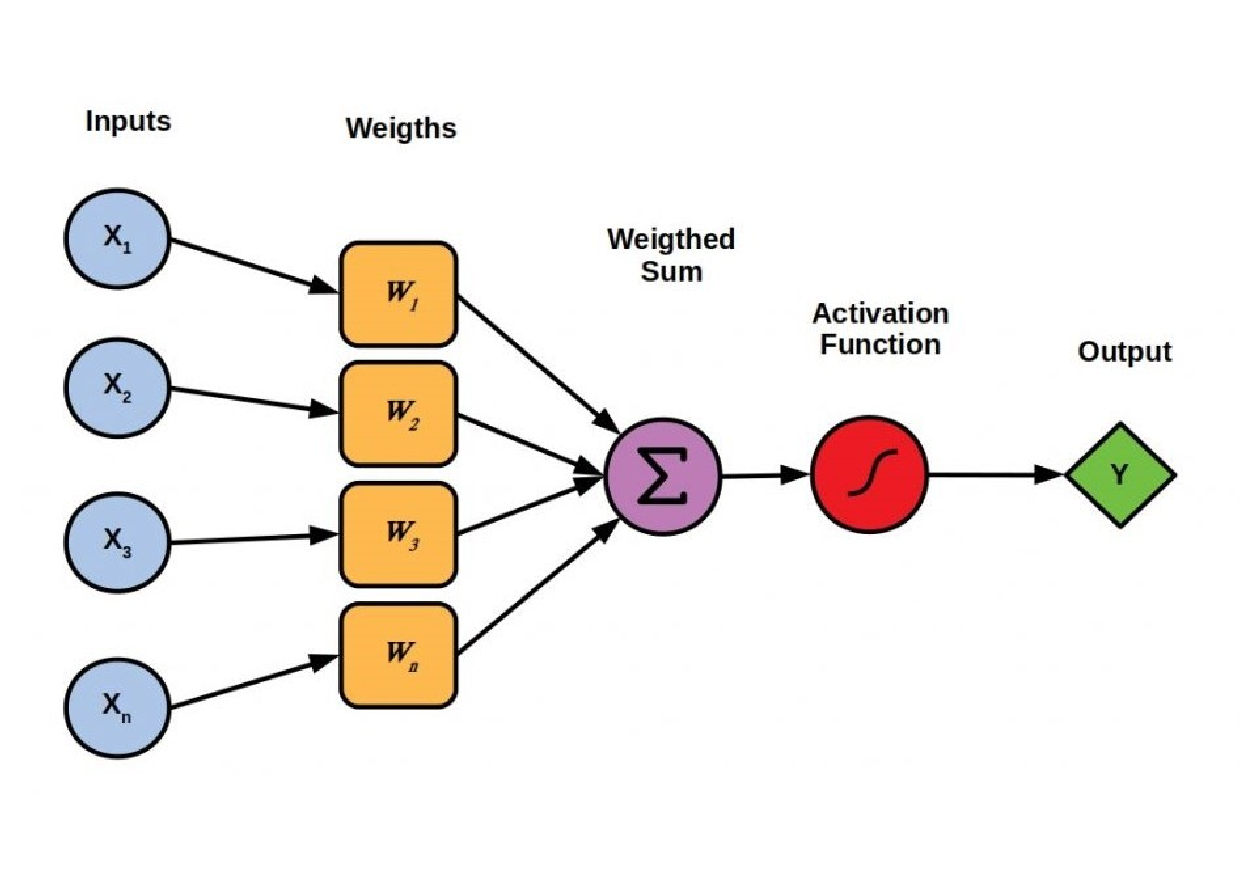
\includegraphics[width=0.6\textwidth]{./Images/perceptron.pdf}
    \caption{Basic modern perceptron scheme}
    \label{fig:perceptron}
\end{figure}

A basic neural network is simply built by putting perceptrons together. By placing them side by side, we get a \emph{single one-layer neural network} and, by putting them in a sequence, we get a \emph{multi-layer perceptrons} (MLP)\cite{MLP}.

In 1974 Paul Werbos introduced the concept of \emph{backpropagation} \cite{Back_werbos}. This is an algorithm that computes the gradient in order to update the parameters or weights of a neural network. Backpropagation first spreads the error from the output layer back to where the parameters need to be updated, by means of the chain rule. Then uses standard gradient descent to update the parameters by a step called the learning rate, but we will discuss these methods later on.

\section{Convolutional Neural Networks}
\label{sec:CNN}

\emph{Convolutional Neural Networks} (CNNs) were first introduced in order to mimic our vision.
\begin{figure}
\centering
\begin{subfigure}{.5\textwidth}
  \centering
  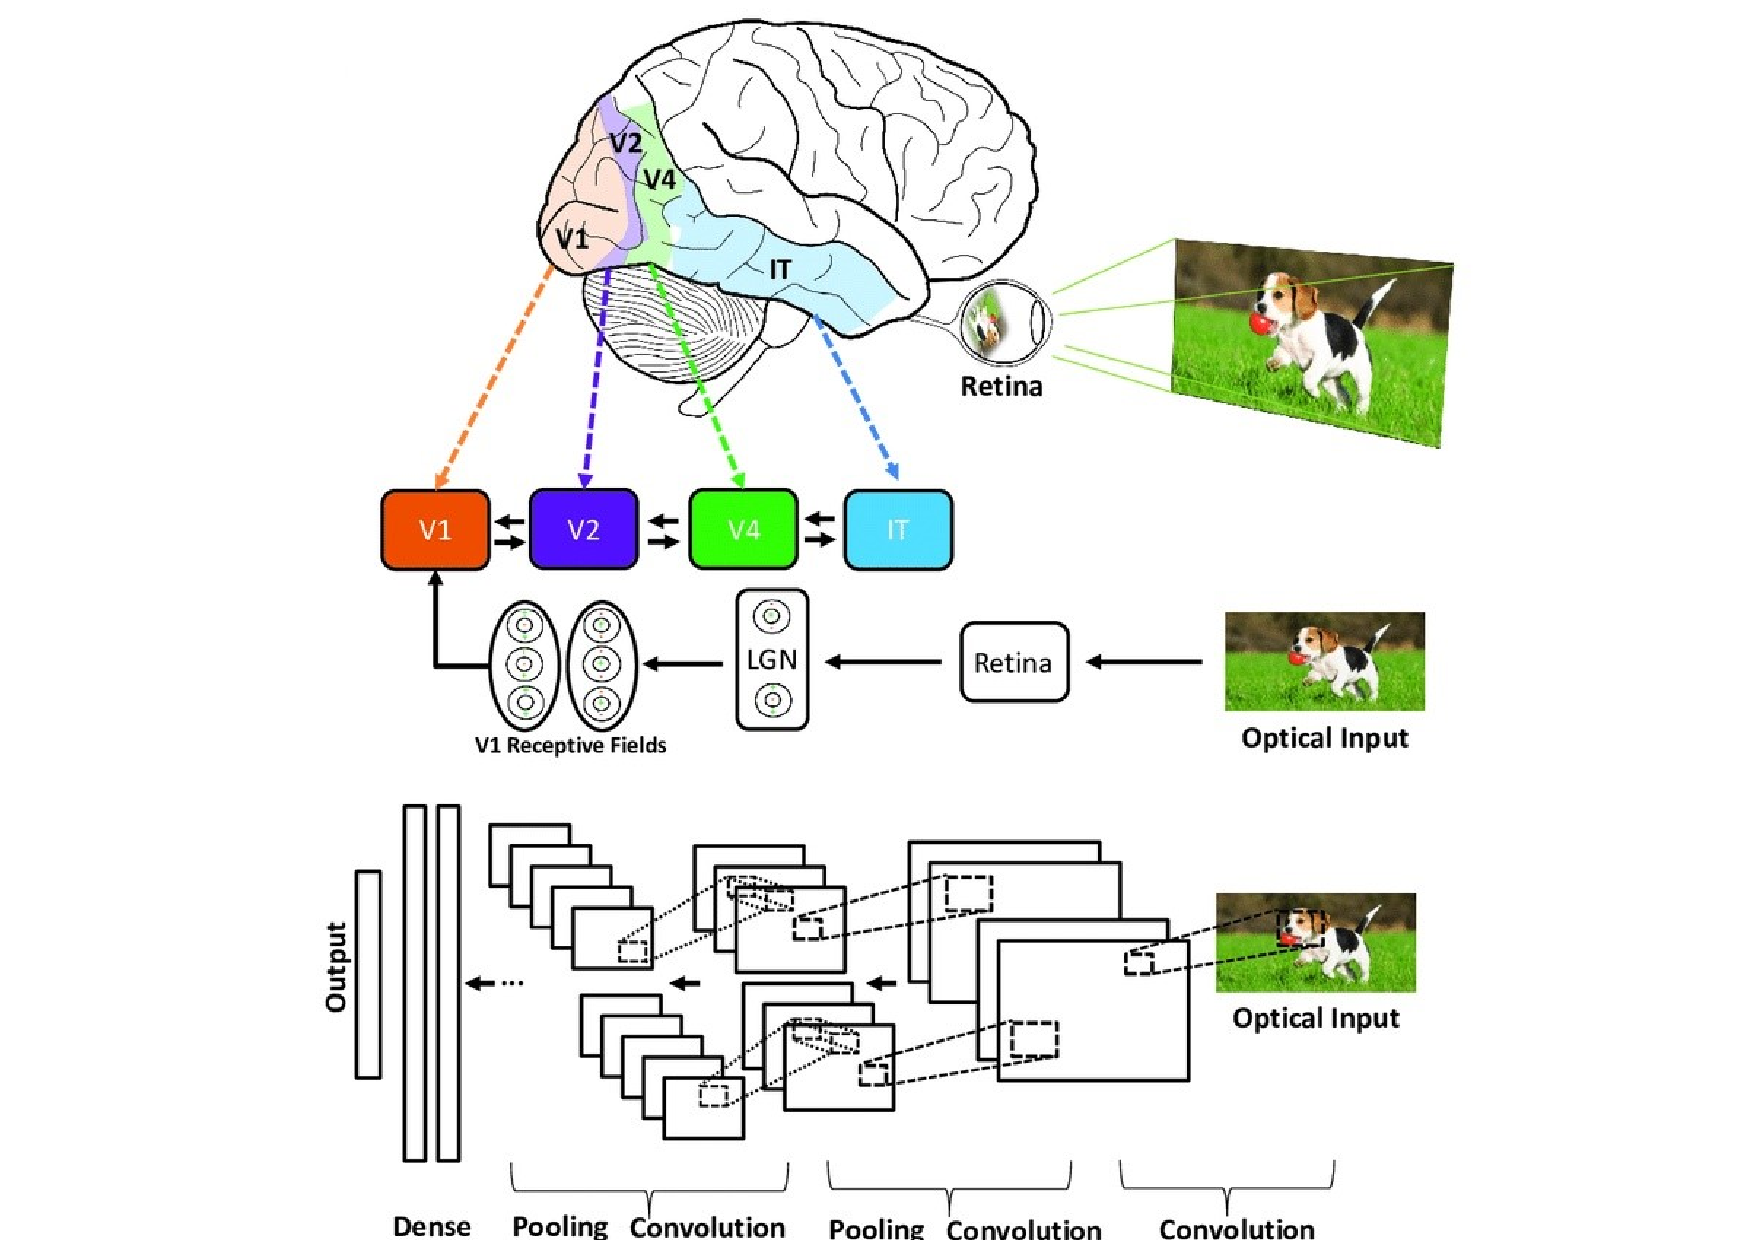
\includegraphics[trim={5cm 7.5cm 5cm 0cm}, clip, width=0.9\linewidth]{Images/visual_cortex.pdf}
\end{subfigure}%
\begin{subfigure}{.5\textwidth}
  \centering
  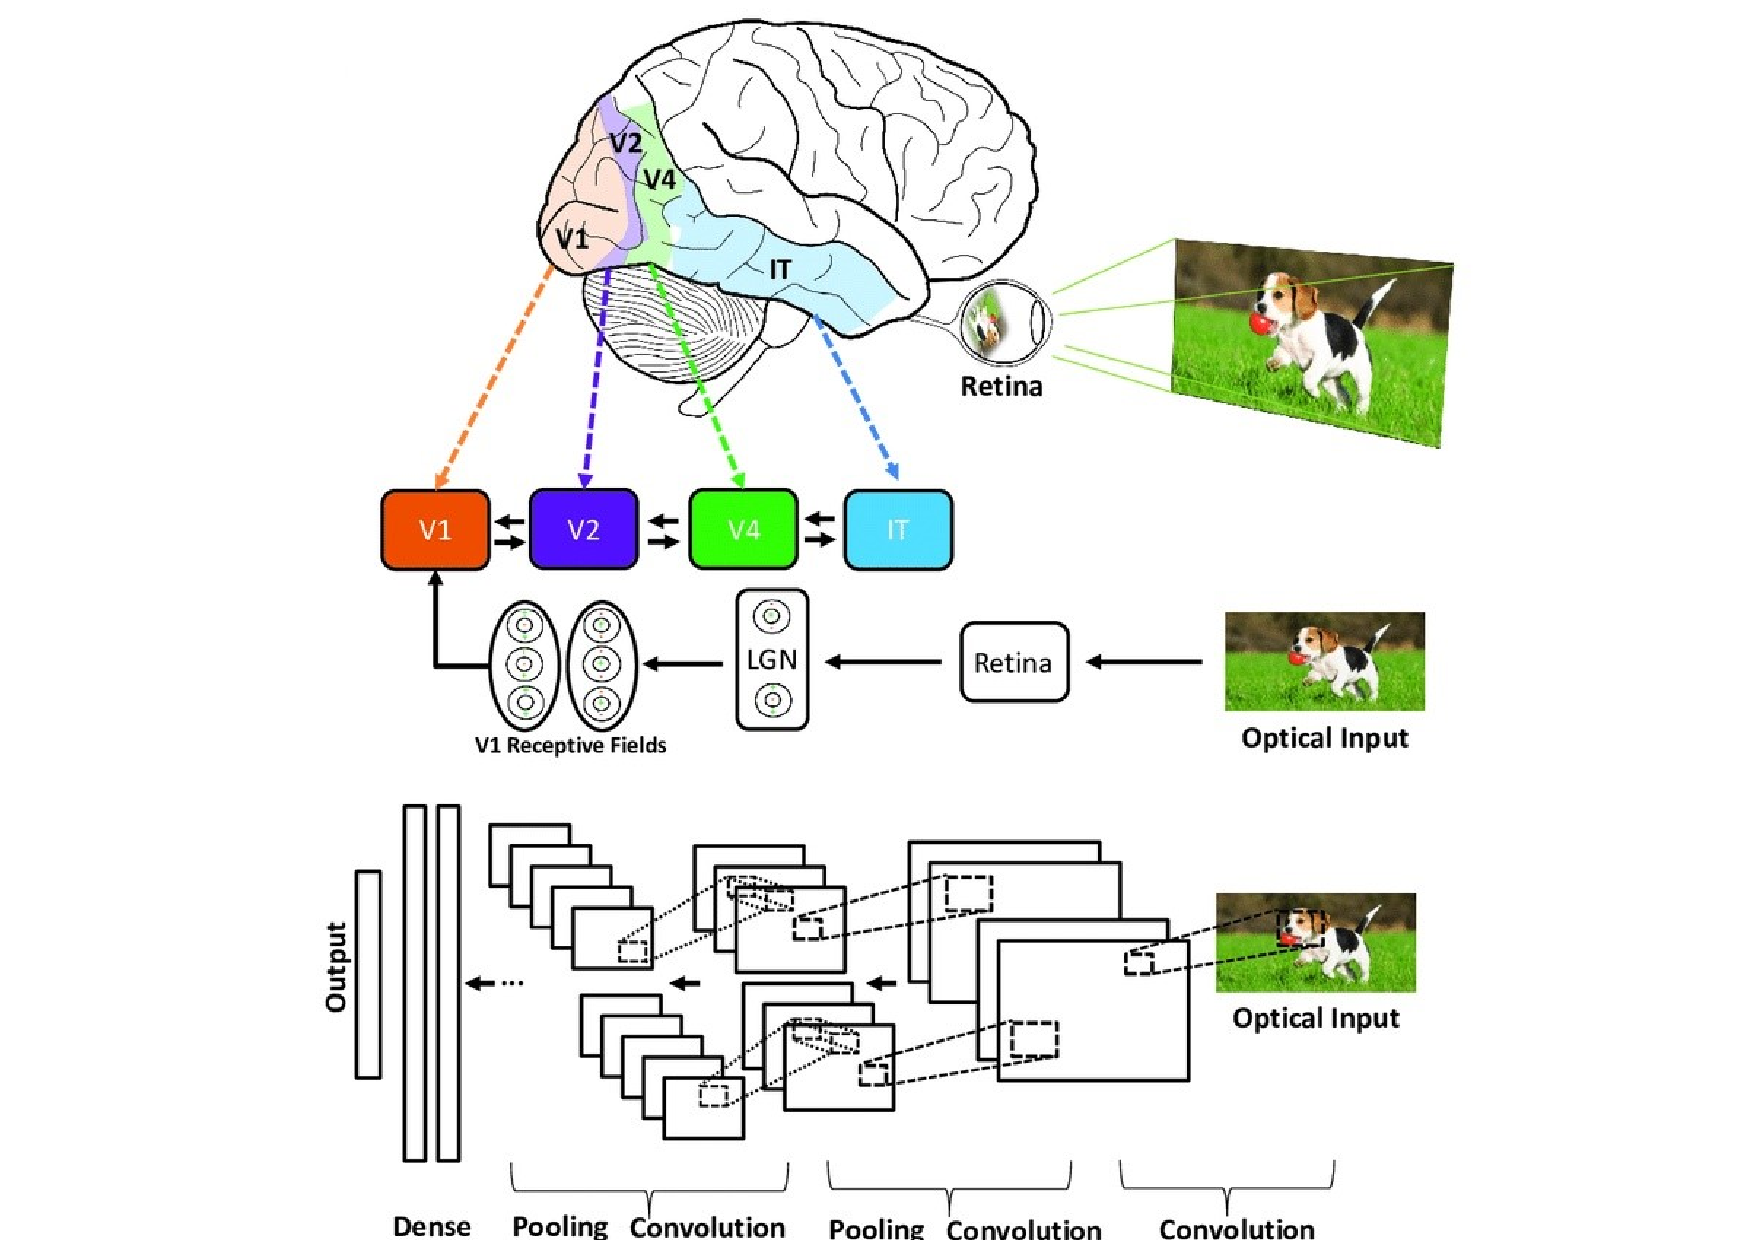
\includegraphics[trim={5.5cm 0 5.5cm 13cm}, clip,width=0.9\linewidth]{Images/visual_cortex.pdf}
\end{subfigure}
\caption{Convolutional neural networks originate from our understanding of the primary visual cortex}
\label{fig:visual_cortex}
\end{figure}
% rather than a human brain. Despite the reason that separate the two families, they both have features similar to the other and use the same methods to learn and categorize objects. 
%They go also under the name of deep learning.
 ``Neocognitron'' \cite{neocognitron} is generally recognised as the model that inspires CNNs on the computation side. It consists of two different kinds of layer: S-layer and C-layer. The former is inspired by the primary visual cortex and works as a feature extractor: it is in fact trained to be responsive to a particular feature of the image. The latter is mainly introduced for shift invariant property of features extracted by the S-layer. The first CNN, known as ``LeNet'', was introduced in the 1990s by Yann LeCun \cite{LeNet}, a postdoctoral computer science researcher. LeNet was able to recognize handwritten digits and was therefore used in banking and postal services.
 \begin{figure}[h]
     \centering
     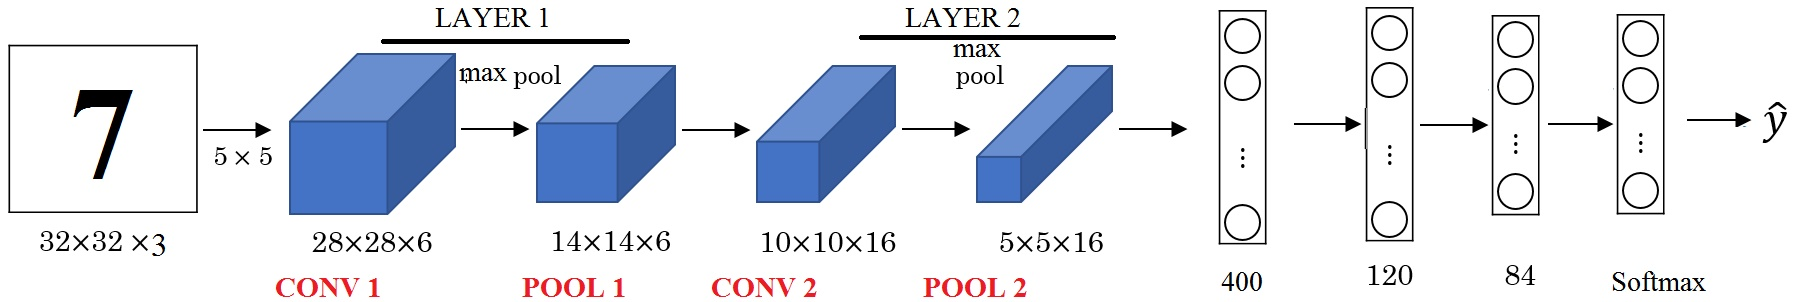
\includegraphics[width = 0.9\textwidth]{Images/LeNet_.jpg}
     \caption{Architecture of a CNN to recognise digits such as LeNet}
     \label{fig:LeNet}
 \end{figure}
 Other successful CNNs, such as AlexNet \cite{AlexNet} or VGG \cite{VGG}, got their popularity through the ImageNet Challenge \cite{ImageNet}, whose goal was to foster the development of CNNs by proposing a challenge regarding image classification task. From \Cref{fig:imagenet} it is clear how neural networks with deeper architectures were a turning point in the history of computer vision algorithms, reducing the classification error from 26\% to 16\% in a few years.

\begin{figure}[h]
    \centering
    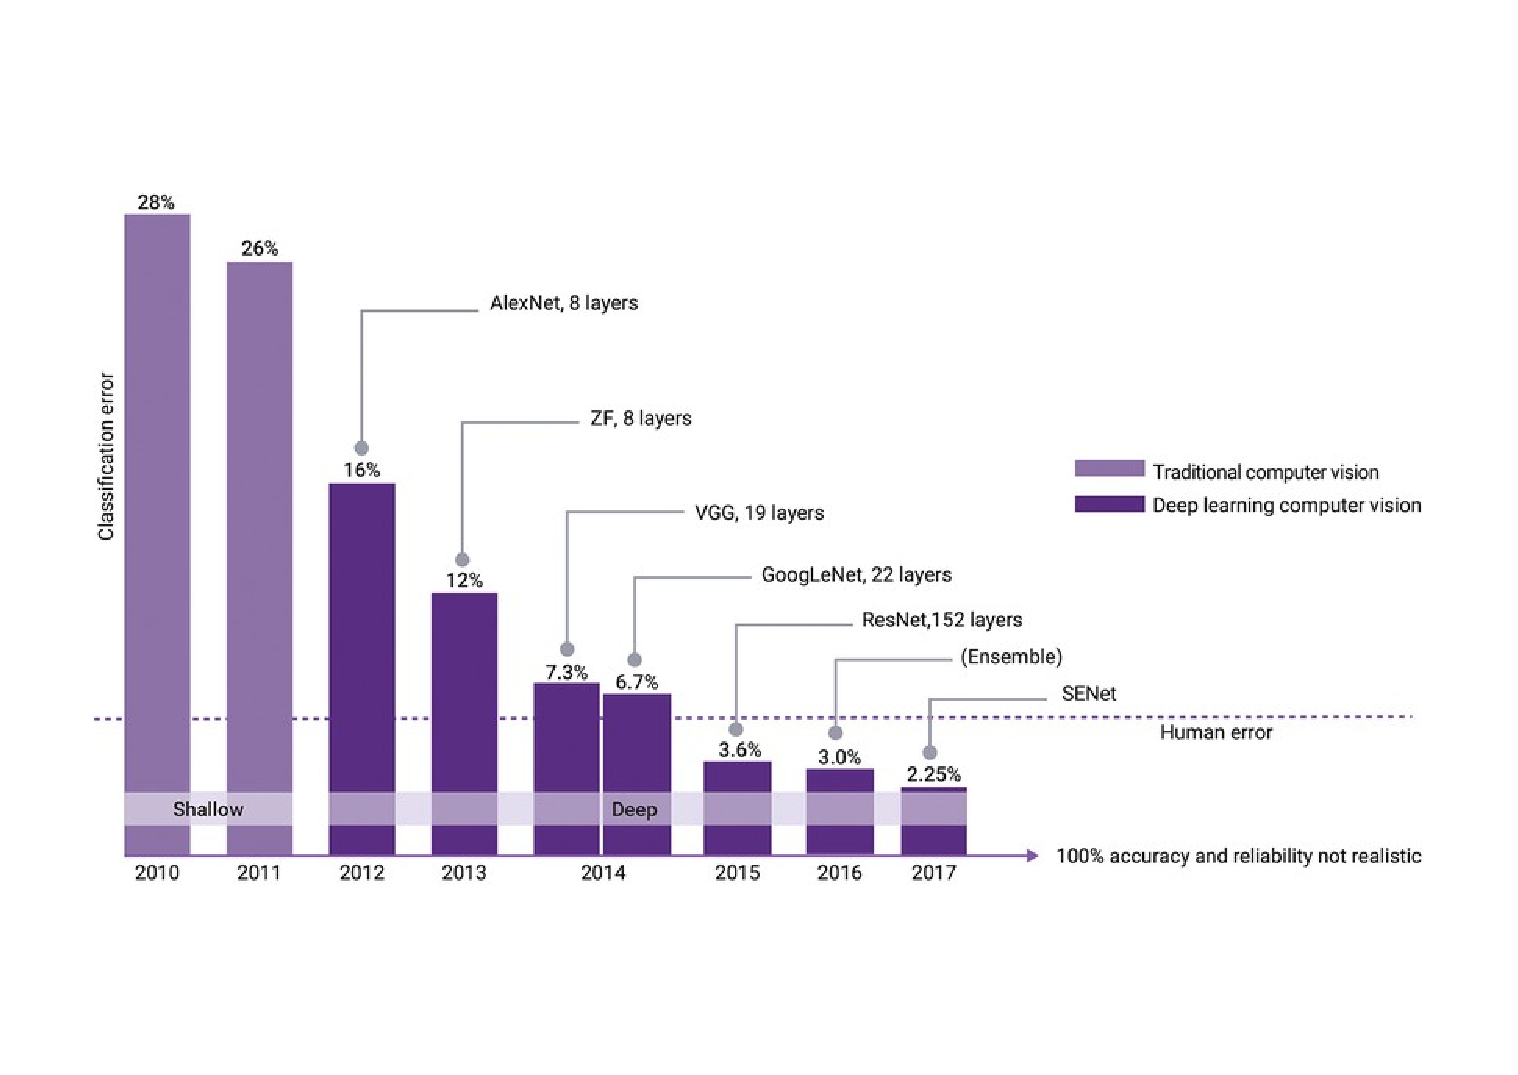
\includegraphics[trim={1cm 3.3cm 1cm 3cm},clip,width=0.9\textwidth]{./Images/ImageNet.pdf}
    \caption{Winners of the ImageNet Challenge through years}
    \label{fig:imagenet}
\end{figure}

\section{Graph Neural Networks: the beginning}
\label{sec:GNN}

Deep learning models are very successful in processing traditional data like images or texts, but they are limited to grid-like data. However, people began to wonder how non-Euclidean data, such as graphs or manifolds, could be processed through some similar mechanism. This led to the creation of a distinct branch of Machine Learning called \emph{geometric deep learning} (GDL), focused on more complex data. The goal is to modify the existing algorithms, in order to handle graphs and manifolds encoding the data. The term ``geometric deep learning'' was first introduced by Micheal Bronstein in his ERC grant in 2015 and then popularized through the paper \cite{Beyound_eucl_data}.
Early forms of \emph{Graph Neural Networks} (GNNs) can be traced back to the 90's, for example Alessandro Sperduti's work \cite{Sperduti_GNN} of 1994, the ``backpropagation through structure'' of Goller and Kuchler \cite{Goller_Kutchler} and the adaptive processing of data structures \cite{Frasconi_GNN}.
Nevertheless, the first actual Graph Neural Network was proposed in 2005 by M. Gori \textit{et al.} to process graphs \cite{Gori}. The first attempt, to generalize neural networks methods on graphs, dates back to 2008 by Scarselli \textit{et al.} \cite{Scarselli}. Later on, in the paper \cite{Bruna_GNN}, Bruna \textit{et al.} proposed the use of spectral CNNs on graphs.
With the spreading of interest towards this new research field, many other algorithms were proposed, such as \emph{Graph Attention Networks} (GATs) \cite{GATs} or graph auto-encoders. This resulted in many applications of GDL to a wide range of practical problems, from biochemistry \cite{BioChem}, skeleton-based human motion recognition tasks \cite{skeleton_motion}, to the recommender systems \cite{reccomender}.

We conclude our history journey with a quote taken from the paper \cite{5_Gs}, written by M. Bronstein, J. Bruna, T. Cohen and P. Veličković:

\begin{displayquote}
``There is a veritable zoo of neural network architectures for various kinds of data, but few unifying principles\ldots, this makes it difficult to understand the relations between various methods, inevitably resulting in the reinvention and re-branding of the same concepts in different application domains.''
\end{displayquote}

\begin{figure}[t]
    \centering
    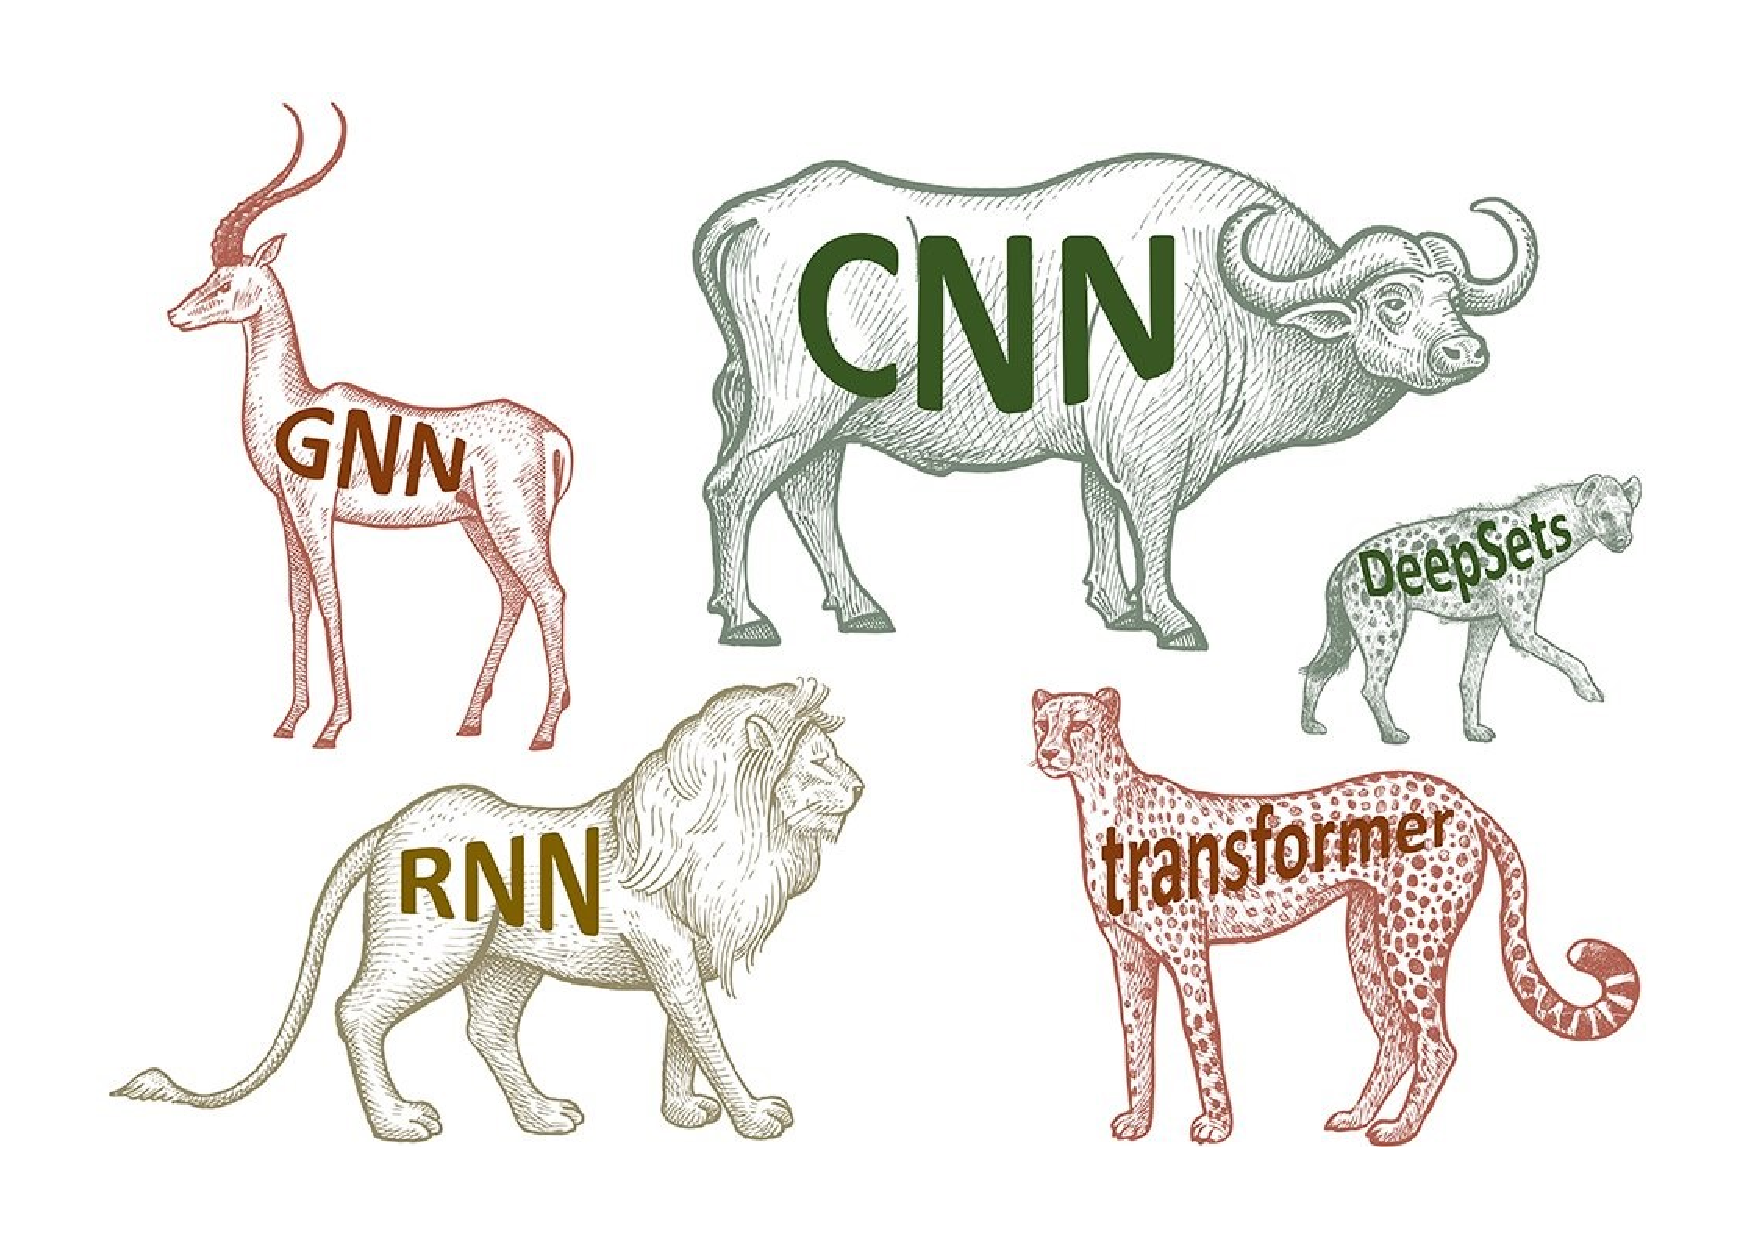
\includegraphics[width=0.6\textwidth]{./Images/NN_zoo}
    \caption{Deep learning today: a zoo of architectures, few unifying principles}
    \label{fig:NN_zoo}
\end{figure}

\section{Datasets}
\label{sec:dataset}

We now introduce few basic concepts common to all neural networks for supervised learning.

\begin{figure}[h]
\begin{minipage}[b]{0.41\linewidth}
\centering
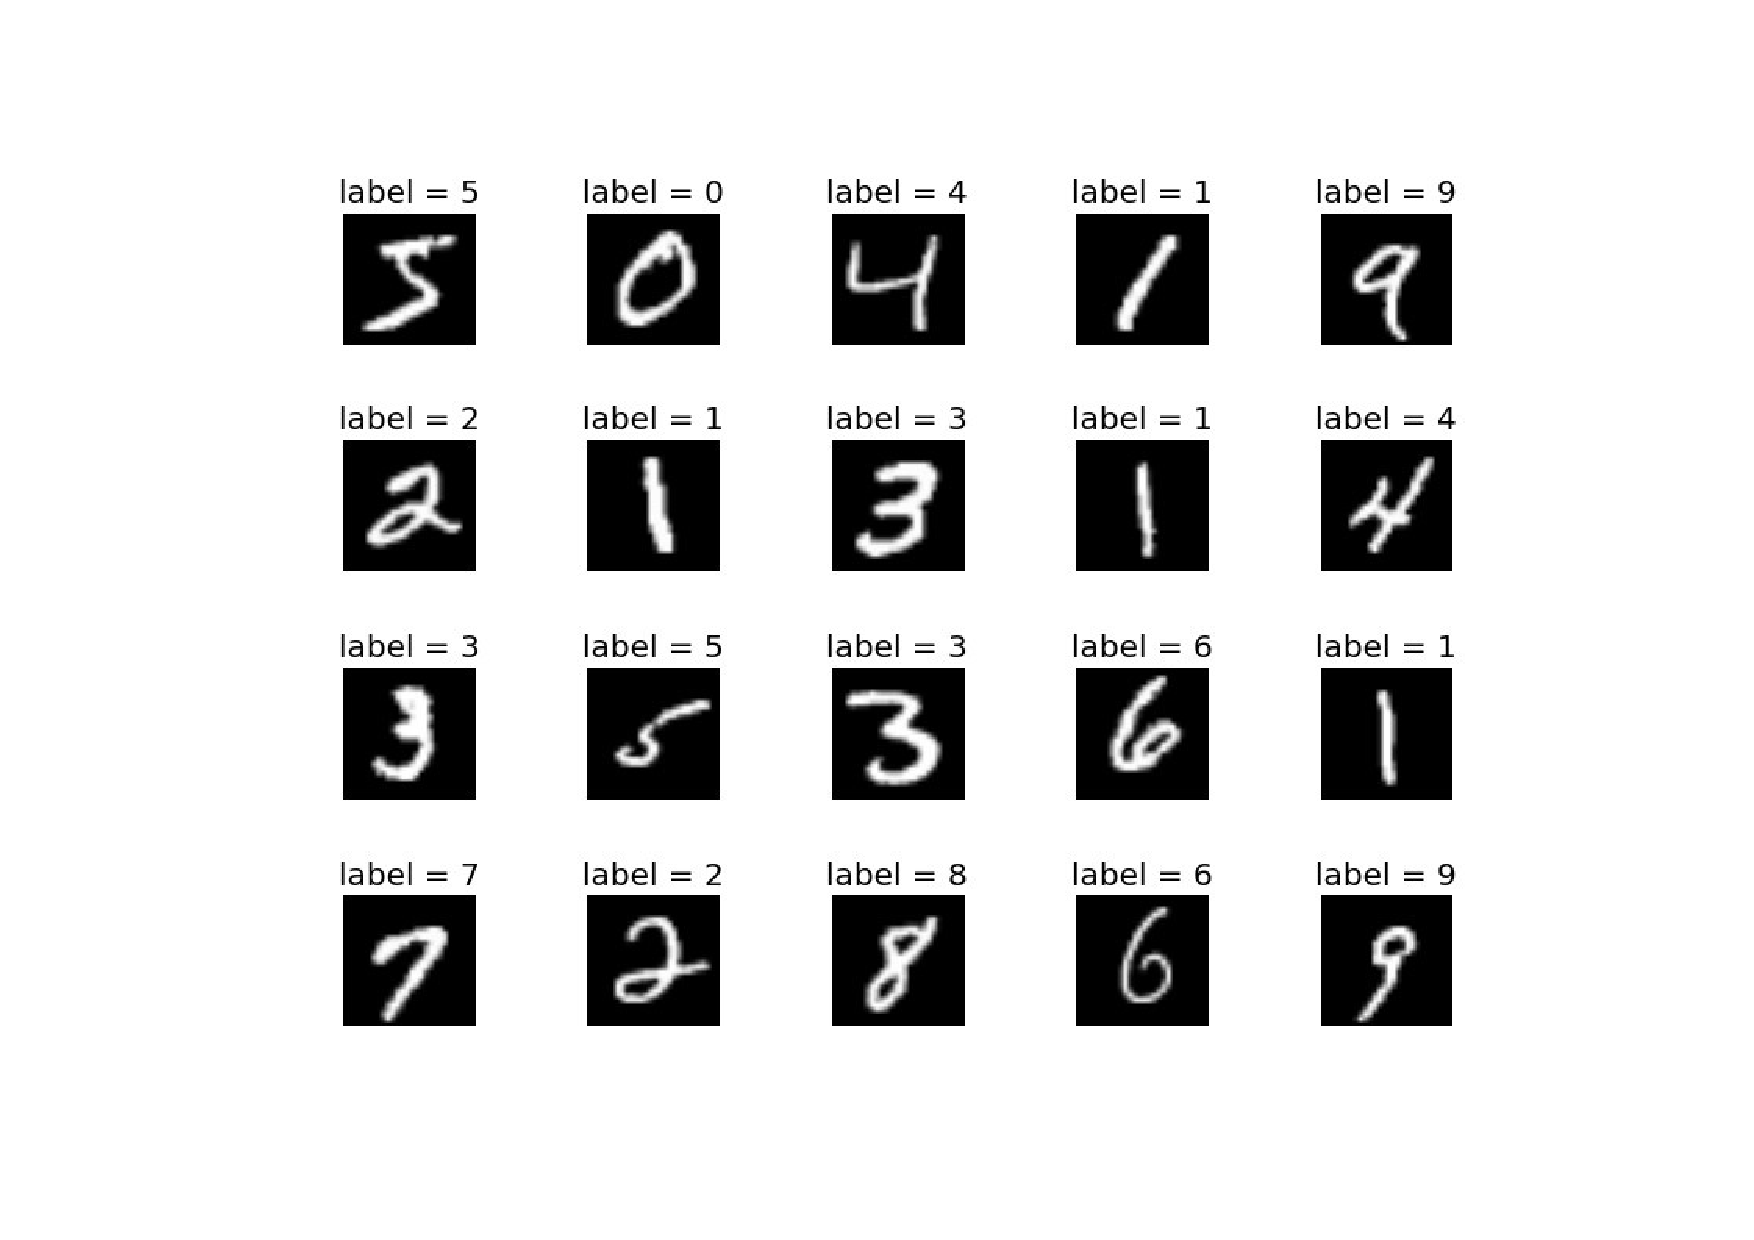
\includegraphics[trim={5.5cm 3.6cm 5cm 3cm}, clip, width=\textwidth]{./Images/MNIST-dataset.pdf}
\caption{Examples of labeled images in the MNIST database}
\label{fig:MNIST dataset}
\end{minipage}
\hspace{0.5cm}
\begin{minipage}[b]{0.54\linewidth}
\centering
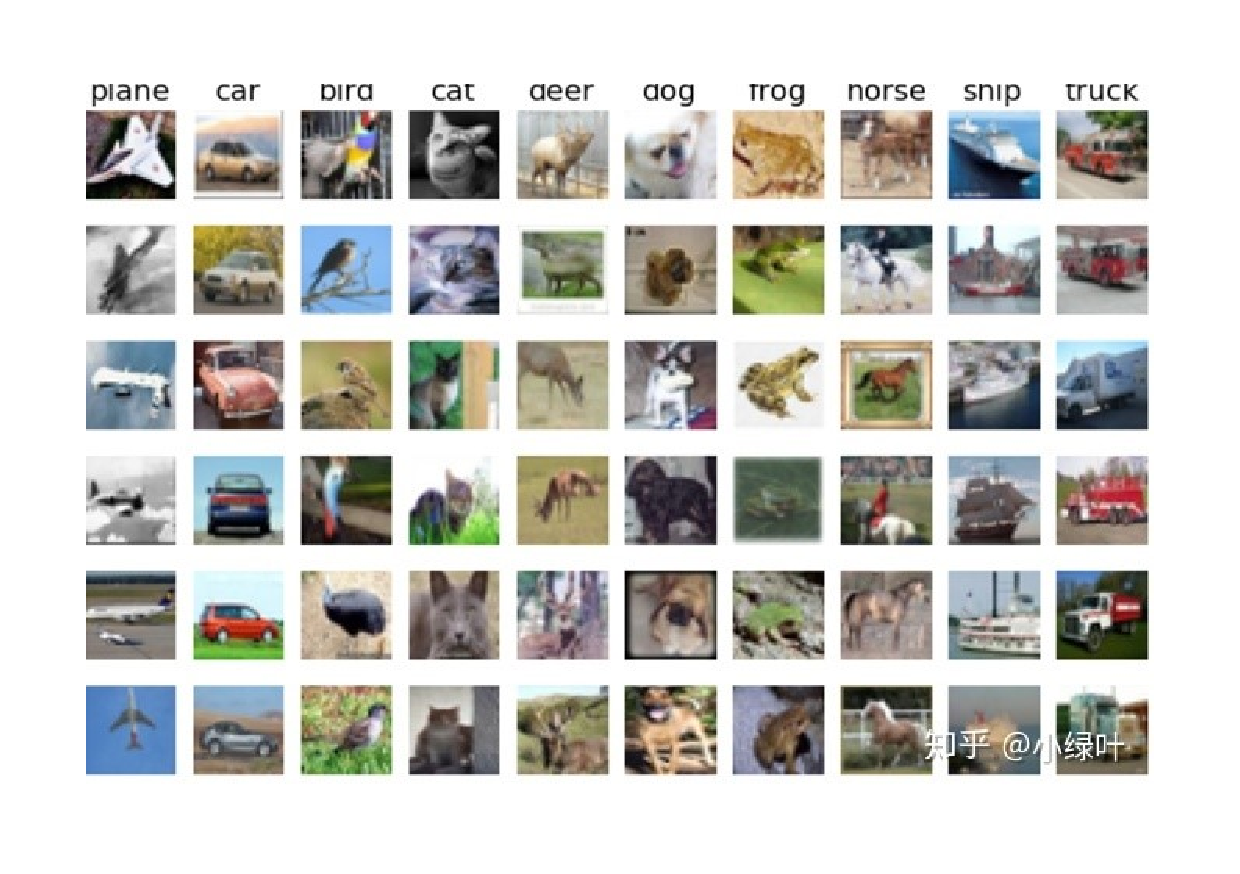
\includegraphics[trim={1.5cm 3.3cm 1.6cm 1cm}, clip, width=\textwidth]{./Images/CIFAR_10_3.pdf}
%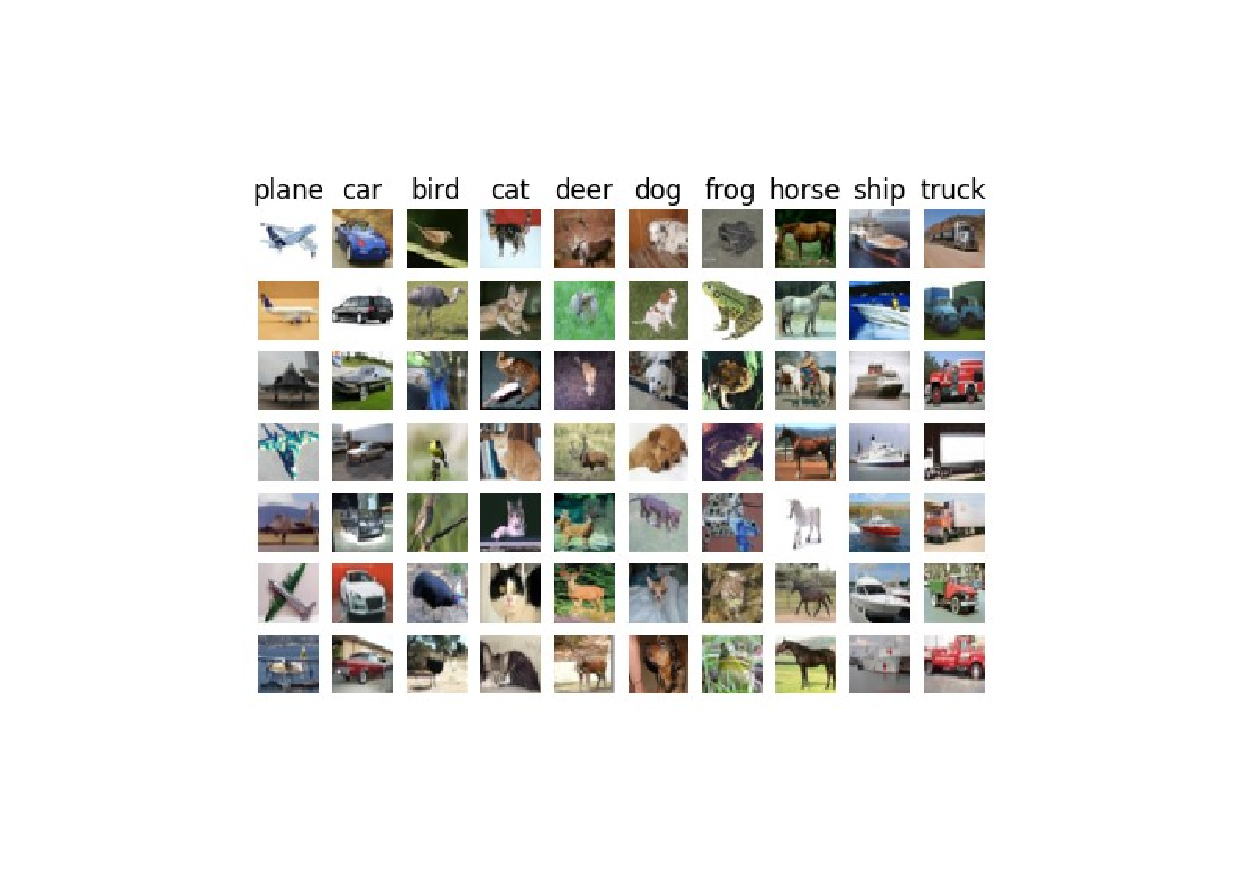
\includegraphics[trim={4.2cm 2.9cm 4.2cm 3cm}, clip, width=\textwidth]{./Images/CIFAR_10_2.pdf}
\caption{Some images in CIFAR-10 dataset divided by class}
\label{fig:CIFAR dataset}
\end{minipage}
\end{figure}
One of the main and most important ingredients is an homogeneous and clearly labelled dataset to train the neural network.
Some benchmark datasets are the MNIST database, the CIFAR-10 dataset \cite{CIFAR_dataset} for CNNs and the Zachary Club and Cora datasets for GNNs, that we will discuss in detail in \Cref{sec:Zachary}. The MNIST dataset, shown in \Cref{fig:MNIST dataset}, contains 70\,000 black and white images, 28\times28 pixels, representing digits from 0 to 9.
Each image is labeled by the digit that represents and the task is to teach the neural network to recognise the hand-written digits.
The CIFAR-10 dataset, instead, is a collection of 60\,000 colored images 32\times32, and the task is to predict what they are showing and classifying it between 10 different classes: cat, dog, bird, deer, frog, horse, ship, truck and plane. In \Cref{fig:CIFAR dataset} are shown the classes in the dataset, as well as 5 random images from each.

A very common and useful way to organize the dataset for a supervised classification task is to split it in 3 parts:

\begin{itemize}
    \item Training set;
    \item Validation set;
    \item Test set.
\end{itemize}

\begin{figure}[h]
    \centering
    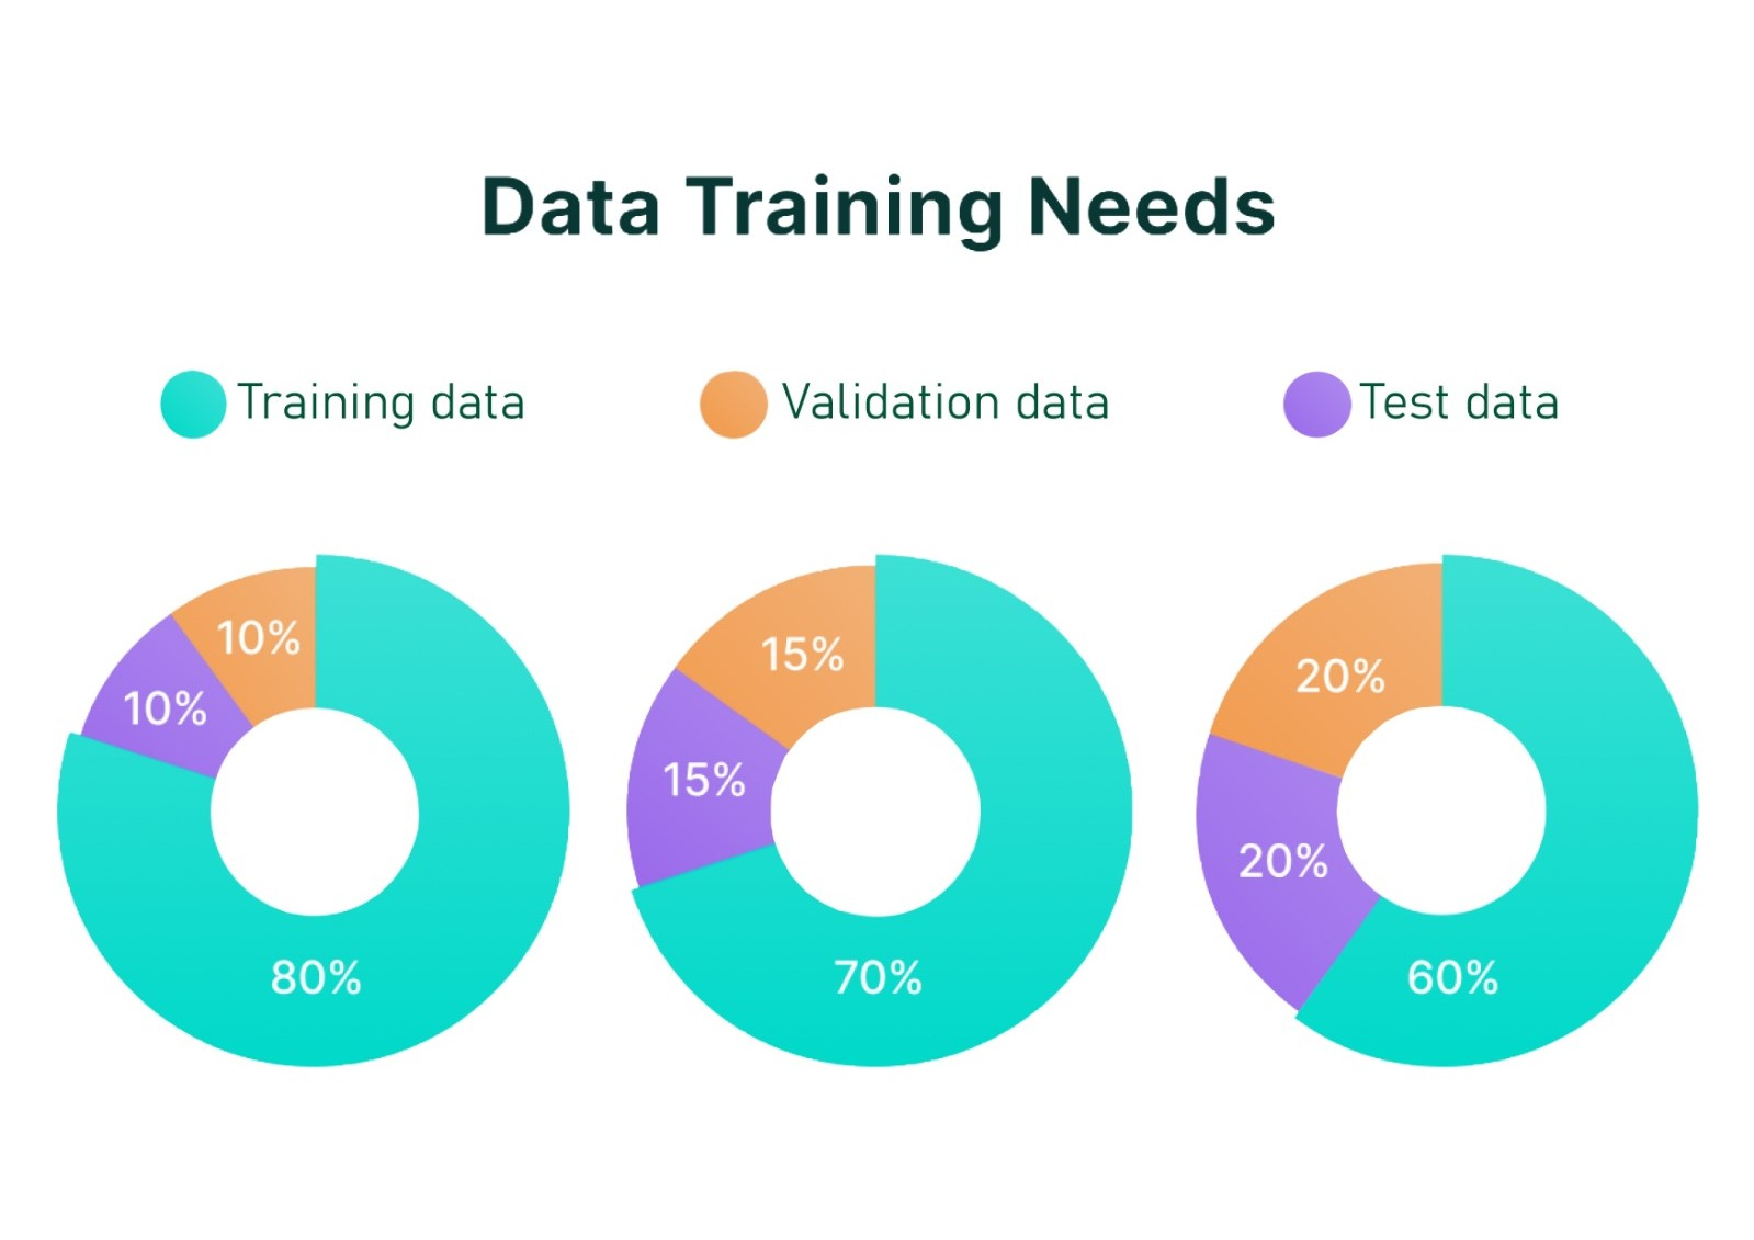
\includegraphics[trim={0 2.9cm 0 6.2cm}, clip, width=0.6\textwidth]{./Images/Data_splitting.pdf}
    \caption{Splitting of the dataset between training, validation and test set}
    \label{fig:train val test}
\end{figure}

The \emph{test set} is set aside from the very beginning and it is used to verify how well the neural network is performing.
The evaluation criterion, called \emph{accuracy}, measures the fraction of correct prediction on the test set over all predictions.


The remaining data is usually further divided into \emph{training} and \emph{validation sets}.
The reason for this is because, generally, when building a neural network, there are many options to choose regarding the architecture. This options consist in choosing values for some variables called \emph{hyperparameters}. For instance, an hyperparameter is the size of a single-layer or the type of loss function to use. We want to choose the options that will make our neural network work best, but we have to be careful not to use the test set for this purpose.
Setting the hyperparameters to maximise the accuracy calculated on the test set will give us excellent results on the training set, but most likely the neural network will not performance so good, when it is used to process other data.
For this reason it is fundamental to evaluate the accuracy of the neural network on the test set only at the very end. It is therefore necessary to pick a validation set aside from the test set, that is what will be used to tune the hyperparameters.

Finally, the training set is used to train the network. In \Cref{fig:train val test} are shown some standards splits of the dataset for CNNs.

\section{Perceptron}
\label{sec:perceptron}

The first perceptron model was introduced in 1958 by Frank Rosenblatt \cite{Rosenblatt} as a mathematical model of a biological neuron. In fact, as a neuron is the computational unit of the brain, similarly the perceptron functions as the neural network unit that can tell whether the input will activate the firing, and therefore give an output, or not.

Since a perceptron is modelled on the working of a neuron, let us focus briefly on how it operates. A biological neuron receives signals from other neurons, through his dendrites. When the incoming signal reaches a certain level of intensity, it triggers the firing of the neuron, that is a sharp electrical potential generated across the membrane called \emph{spike}. This impulse travels through the axon and then ramifies into dendrites of other connected neurons as shown in \Cref{fig:biological_model}. In this way, the neurons communicate via dendrites and axons and together create a network able to spread a signal made of more than 100 trillion connections in the average human brain.

\begin{figure}[h]
\centering
\begin{subfigure}{.5\textwidth}
  \centering
  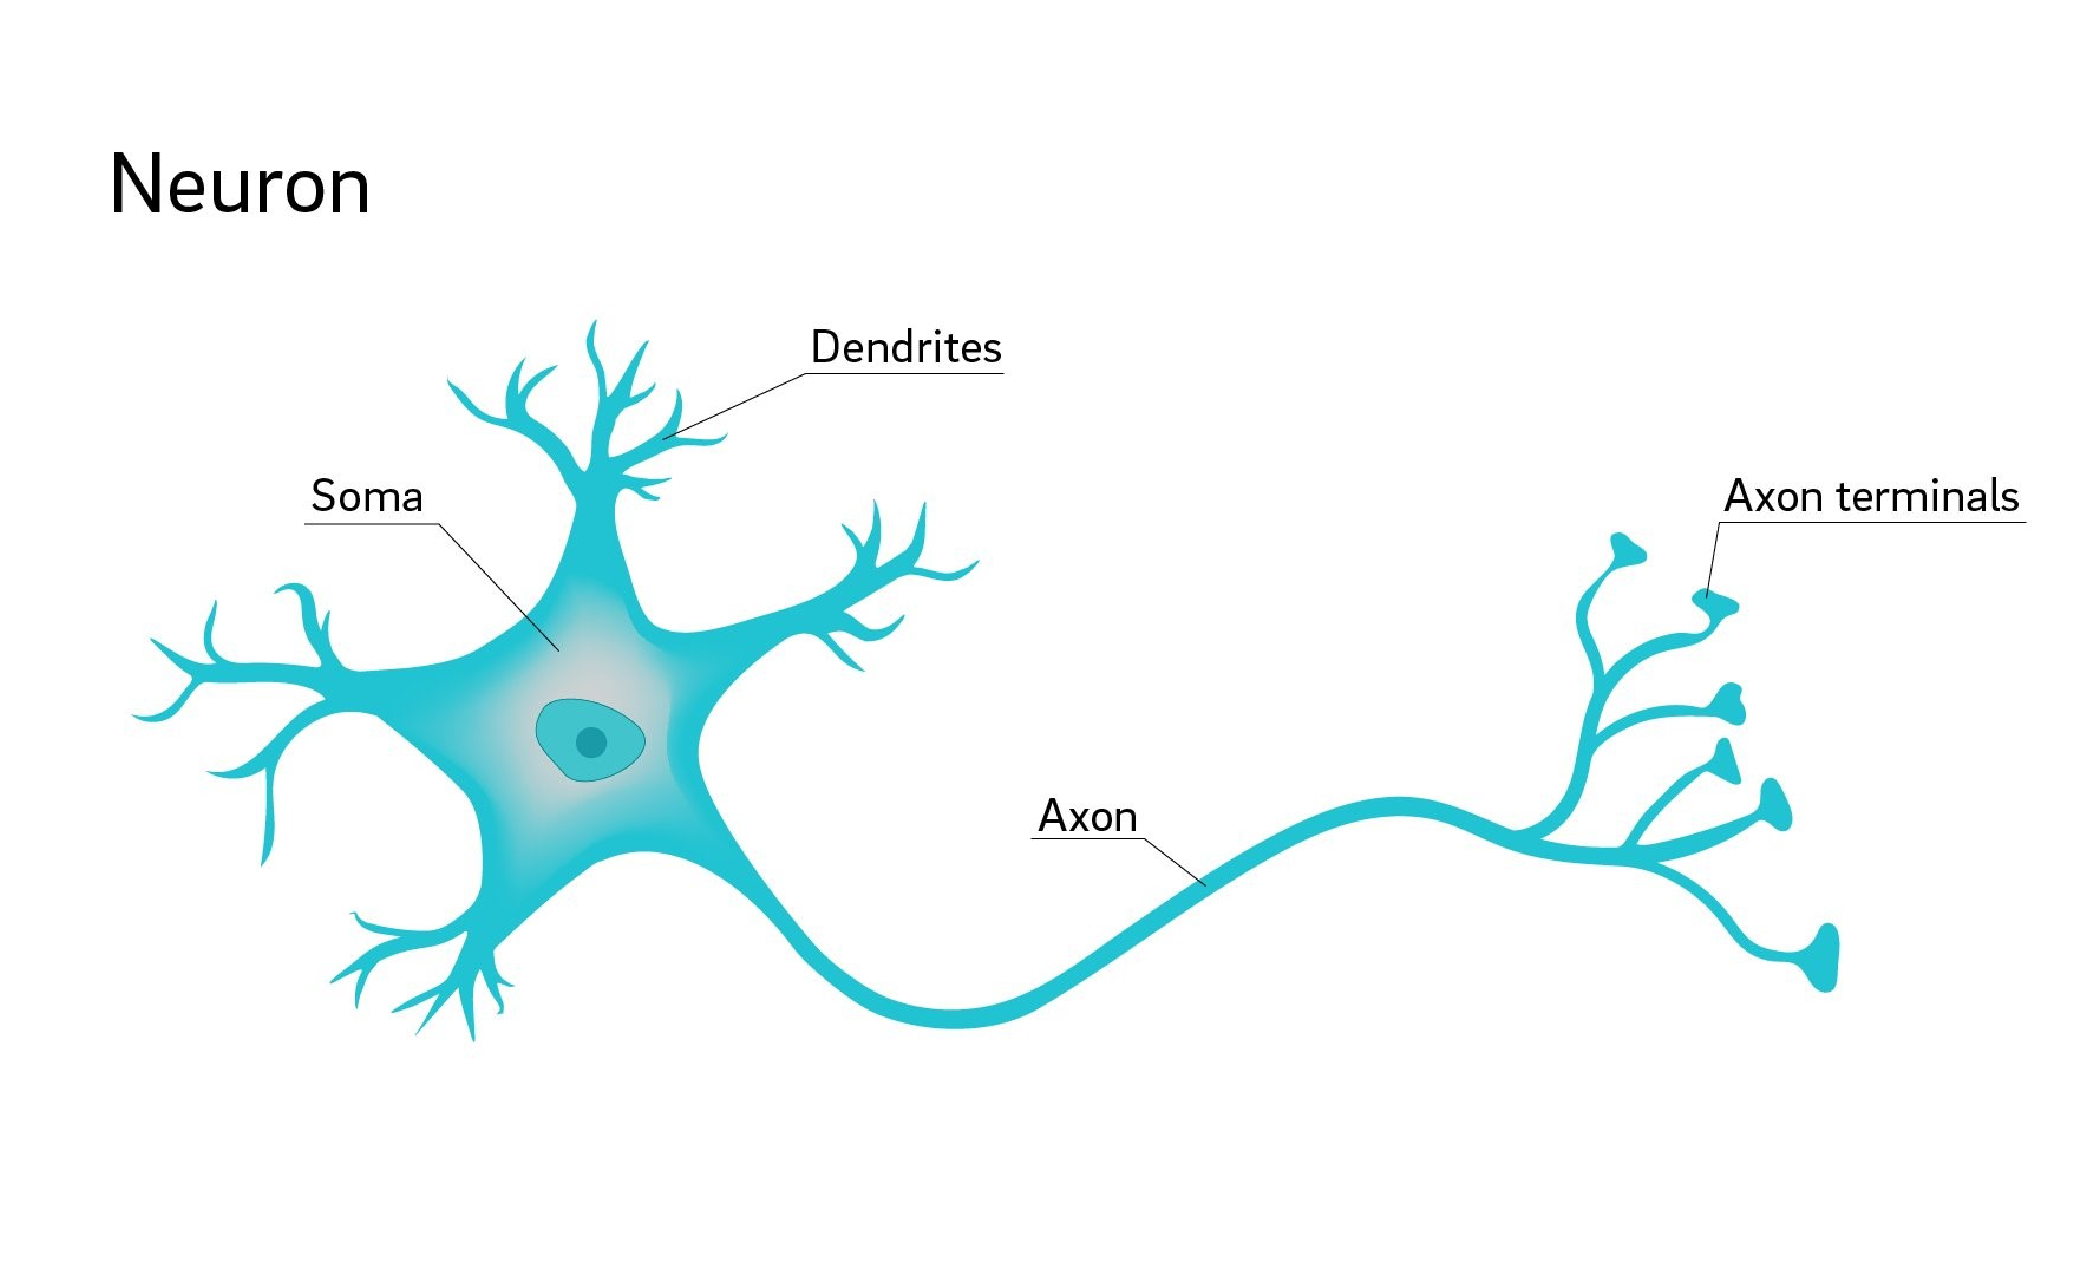
\includegraphics[width=0.9\linewidth]{./Images/neuron.pdf}
  \caption{Biological model}
  \label{fig:biological_model}
\end{subfigure}%
\begin{subfigure}{.5\textwidth}
  \centering
  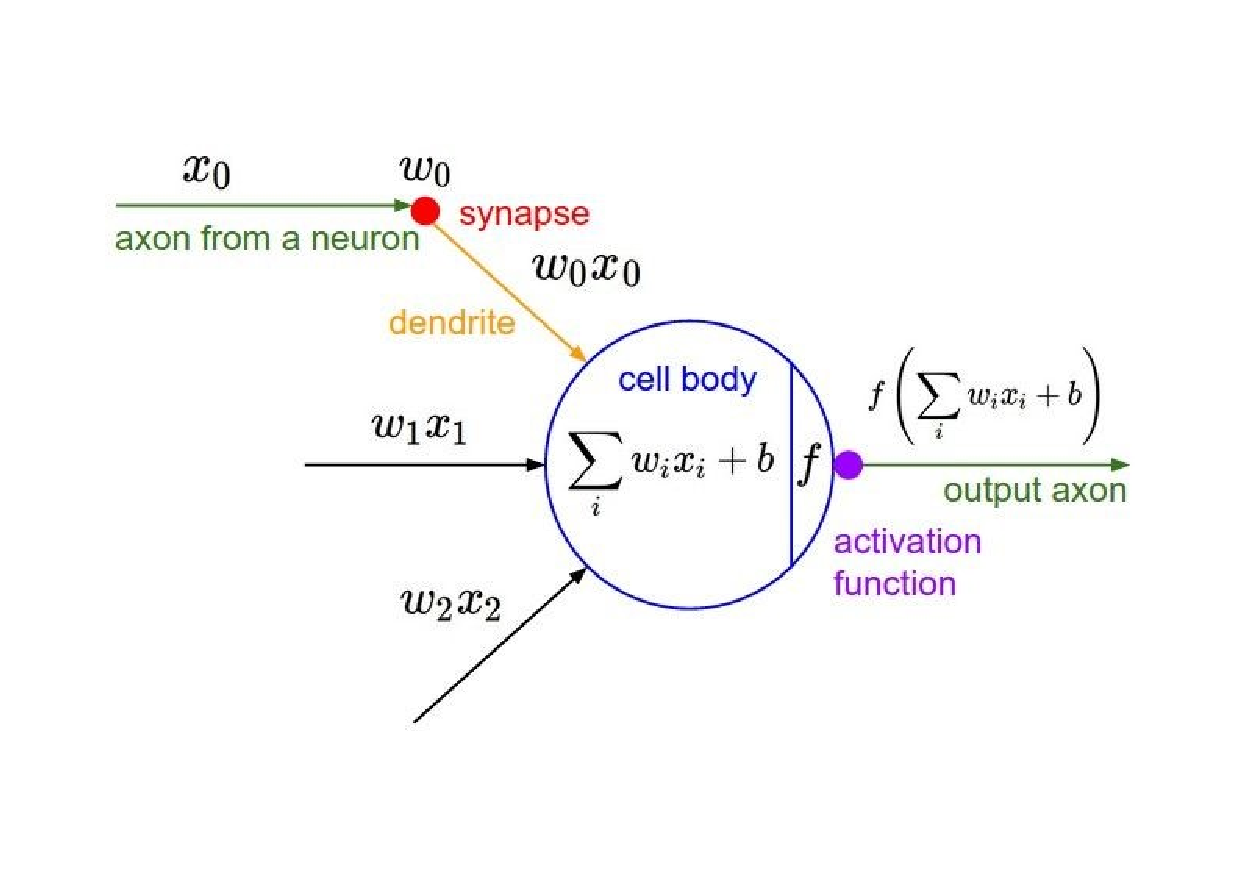
\includegraphics[trim={0 2.2cm 0 0}, clip,width=0.9\linewidth]{./Images/perceptron_stanford.pdf}
  \caption{Mathematical model}
  \label{fig:math_model}
\end{subfigure}
\caption{Two models of a brain neuron}
\label{fig:neuron_models}
\end{figure}

As mentioned before, the perceptron was introduced in order to mimic the working of the biological neuron. Being the mathematical model, it is composed of the main features as described before, as illustrated in \Cref{fig:math_model}.
If a neuron receives an input signal $x_i$ from another neuron, the signal will travel through the dendrite.
In order to mimic the synaptic strength, we multiply the signal for the weight $w _i$ associated with the dendrite.
Since a single neuron receives input signals from thousand of dendrite at the same time, we simulate this behaviour by summing them, to obtain the total signal arriving at the neuron, that can be written as: $\sum_i w_i x_i + b$ ($b$ is the bias term).
To simulate the firing of the biological neuron, when the input reaches a certain threshold level, we use an \emph{activation function $f$}.

\begin{figure}[h]
    \centering
    \resizebox{0.6 \textwidth}{!}{
    \begin{tikzpicture}
    \centering
    \begin{axis}[
        axis x line=center,
        axis y line=center,
        %xtick={-5,-4,...,5},
        %ytick={-5,-4,...,5},
        xlabel={$x$},
        ylabel={$y$},
        xlabel style={below right},
        ylabel style={above left},
        xmin=-3.5,
        xmax=3.5,
        ymin=-1.5,
        ymax=2.5,
        xlabel = \(x\),
        ylabel = {\( y \)},
        legend style={at={(1.03,1)},anchor=north west,draw=black,fill=white,align=left}]
    \addplot [
        domain=-3.5:3.5, 
        samples=100, 
        color=green,
        ]
        {1/(1+exp{-x})};
        \addlegendentry{$\sigma(x)$};
    \addplot [
        domain=-3.5:3.5, 
        samples=100, 
        color=red,
        ]
        {(exp{+x}-exp{-x})/(exp{+x}+exp{-x})};
        \addlegendentry{$\tanh{(x)}$};
    \addplot [
        domain=0:3.5, 
        samples=100, 
        color=blue,
        ]
        {x};
    \addplot [
        domain=-3.5:0, 
        samples=100, 
        color=blue,
        ]
        {0.1 * x};
        \addlegendentry{$\text{Leaky ReLU}(x)$};
    \end{axis}
    \end{tikzpicture}
    }
    \caption{Activation functions}
    \label{fig:activation func}
\end{figure}
Here are some of the most famous activation functions, whose graphs are shown in \Cref{fig:activation func}:
\begin{itemize}
    \item \textbf{Sigmoid}. $\sigma (x) = 1/(1+ e^{-x})$.
    \item \textbf{Tanh} $\tanh(x)= 2\sigma (2x)-1$
    \item \textbf{Leaky ReLU} $f(x)=\begin{cases}
    \alpha x  & \text{if  } x<0 \\
    x & \text{otherwise}
    \end{cases}$
      where $\alpha \ll 1$.
\end{itemize}

The next step to build a neural network is to put perceptrons together as it happens for neurons in the human brain. By placing them side-by-side, we get a single layer.
Two neurons belonging to the same layer are generally not connected.
If we stack the layers in a sequence, we build a MLP (Multi-Layer Perceptrons), also called \emph{Artificial Neural Networks} (ANNs).
Typically these networks have fully-connected layers, which means that each neuron in a layer sends his output signals to all of the neurons in the following layer, as shown in \Cref{fig:MLP}.
Note how the neurons are arranged in lines.
The neurons in between the input and the output layers form what are called \emph{hidden layers}.

\begin{figure}
    \centering
    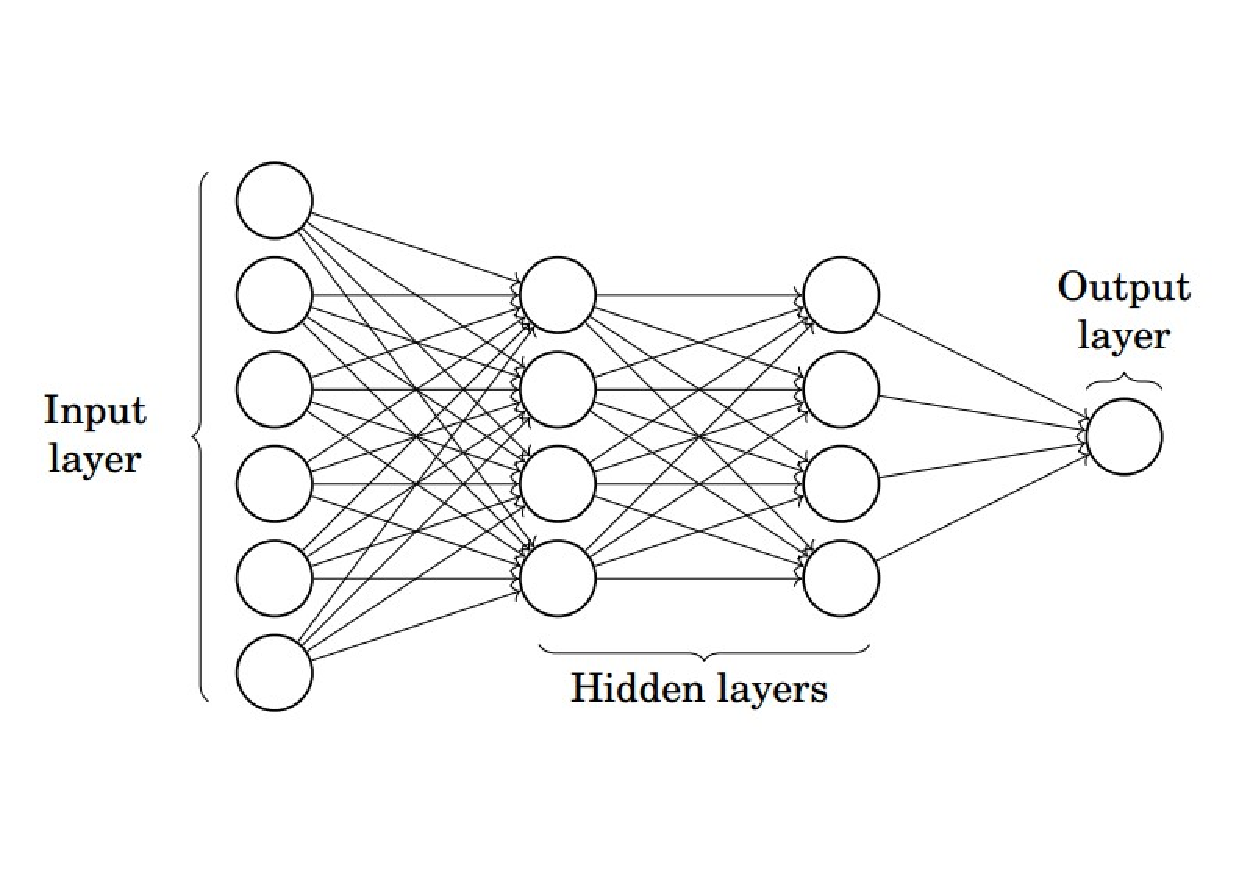
\includegraphics[trim={0 2.7cm 0 2.7cm}, clip, width=0.5\textwidth]{./Images/Multi_Layer_Perceptron.pdf}
    \caption{Example of a MLP}
    \label{fig:MLP}
\end{figure}

This is the basic idea which is behind almost all of the deep learning architectures.
In this way, we are able to build many kinds of neural networks, by just changing the size or the number of hidden layers.
In CNNs for image processing, for example, the neurons are not arranged in one row, but they acquire also a depth dimension, forming 3D layers.

\section{Training}
\label{sec:training}

The previous sections give us enough information to understand the fundamental bases of the training process.
In order for a neural network to learn, there has to be an element of feedback involved.
The idea is to compare the desired outcome with what the network produces and to use the difference between such outcomes to modify the parameters of the network in order to improve its accuracy.

To clarify the concepts, let us consider a simple task such as the classification of the CIFAR-10 images.
An image consists of pixels and the color of each pixel is defined by three numbers representing the three color channels (Red, Green, Blue).
Therefore, a CIFAR-10 image is determined by 32\times32\times3 = 3072 numbers that can be arranged in a vector $\textbf{x}_i$.
%In addition, having 50\,000 images in the training set, we can arrange our vectors in a 3072\times50\,000 matrix $\textbf{x}$.
This relatively easy problem becomes much more difficult when working with graph-like data, as we shall see later on.

Once we have stretched our image into a 3072-dimension vector $\textbf{x}_i$, we can insert it in the input layer and perform the forward pass.
Recall that a perceptron executes the sum of its input signals as $\sum_i w_i x_i + b$, where $x_i$ is the signal coming from the $i$-th neuron of the previous layer, $w_i$ the weight of the connection and $b$ represents the bias.
We can write the operation of passing the signal from a layer to the next one in a more compact notation, using vectors and matrices, as
\begin{equation}
    \textbf{y} = W \textbf{x} + \textbf{b}
    \label{eq:forward}
\end{equation}

where $\textbf{x}$ is the input signal represented by a vector, $\textbf{y}$ is the output signal, that is $y_k$ stands for the signal received by the $k$-th neuron in the next layer.
$W$ and $\textbf{b}$ contain the parameters and they represent, respectively, the weight matrix and the bias vector.
In particular, $W_{ij}$ stands for the connection from the $j$-th neuron of a layer to the $i$-th neuron of the next one.
In \Cref{fig:matrix_multiplication} is shown a simple example of forward pass process from a layer with 4 neurons to another layer with 3 neurons.
In fact, in \Cref{fig:matrix_multiplication} we start with a 4-dimensional vector $\mathbf{x}$ representing the signal and, after the matrix multiplication, we end up with a 3-dimensional vector as a result.
Afterwards, the outcome of \Cref{eq:forward} has to go through one of the activation functions discussed in \Cref{sec:perceptron}, and only then we have computed a forward pass of the signal between two layers, that is basically one matrix multiplication followed by a bias offset and an activation function.
We can therefore write the forward pass in a more complete way as
\begin{equation*}
    \mathbf{x}_{i+1} = f\left( W_i \mathbf{x}_i + \mathbf{b}_i \right)
\end{equation*}
where $\mathbf{x}_i$ stands for the signal on the $i$-th layer of the neural network, while $W_i$ and $\mathbf{b}_i$ are the weight matrix and bias vector of the $i$-th layer.
In simple deep learning architectures, this process has to be repeated for every pair of connected layers, until reaching the output layer.

\begin{figure}
    \centering
    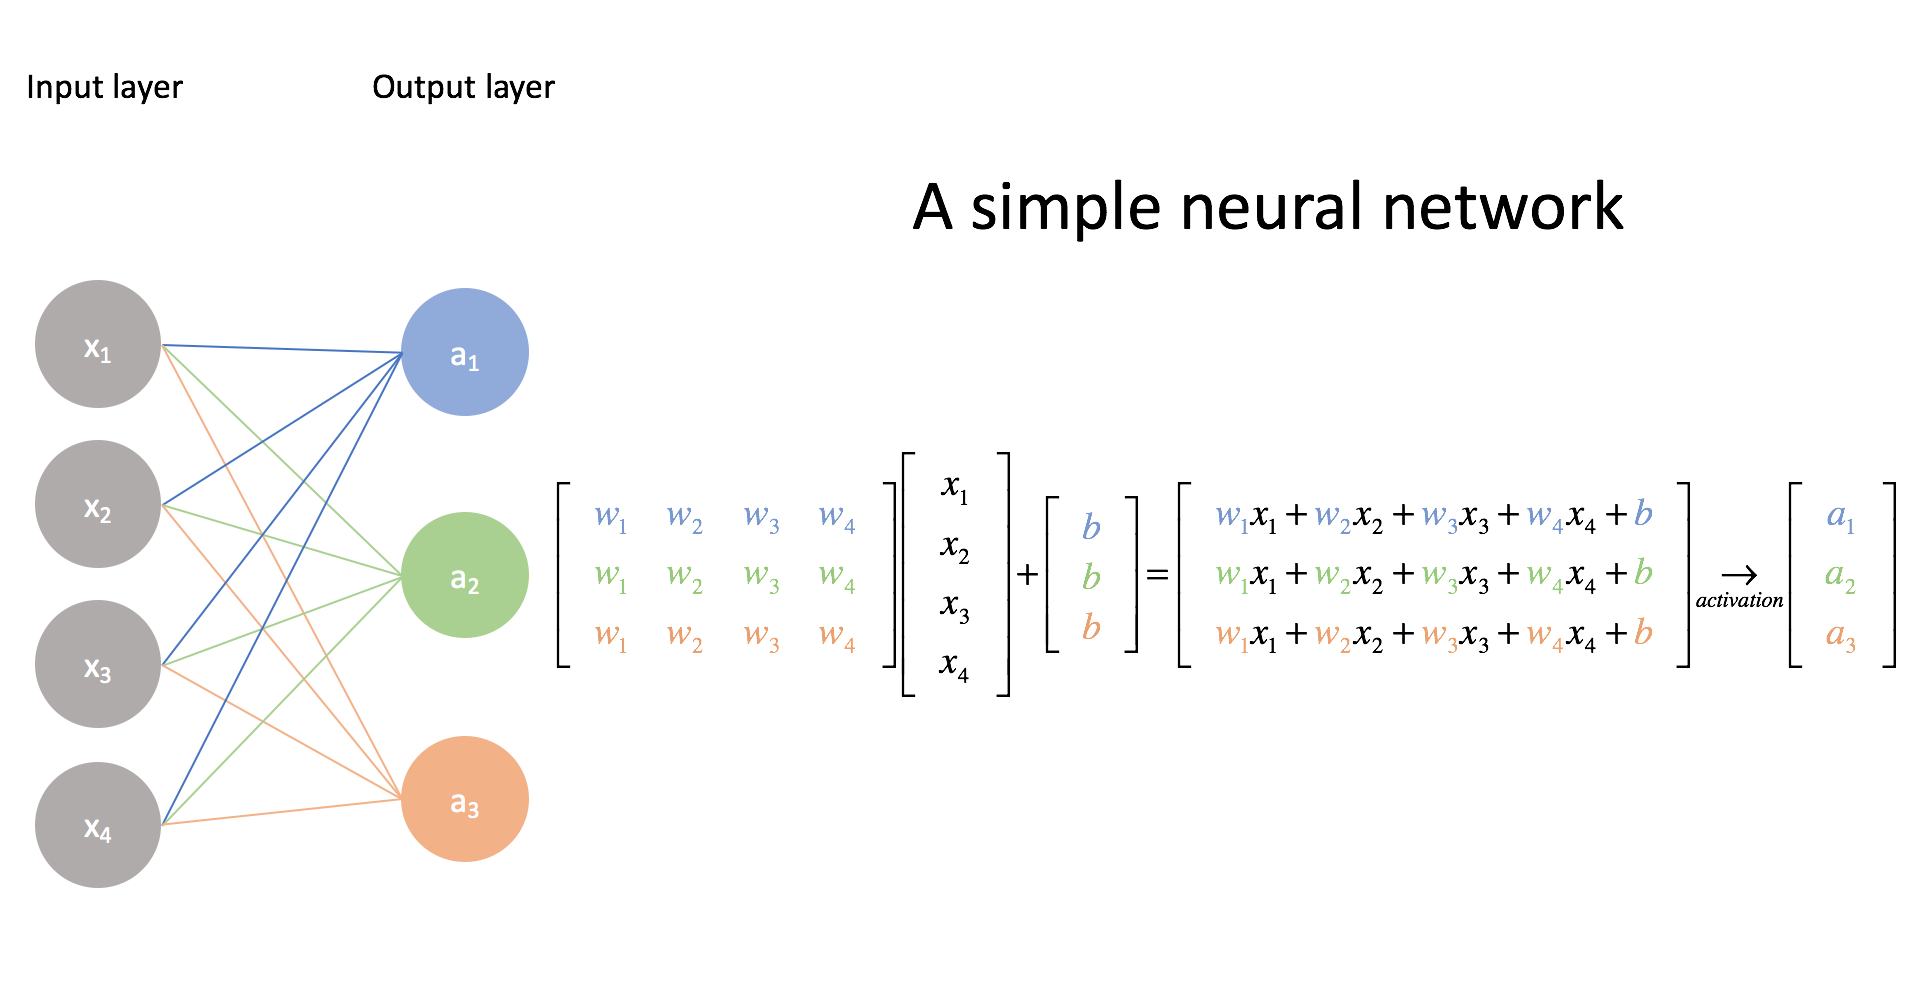
\includegraphics[width=0.95\textwidth, trim={0 1.5cm 0 4.8cm},clip]{./Images/Matrix representation.png}
    \caption{Matrix multiplication in forward pass process}
    \label{fig:matrix_multiplication}
\end{figure}

Typically, the values of the last hidden layer are mapped into the class scores in the output layer through a \emph{linear classifier}, that is simply a   forward pass without the activation function (\Cref{eq:forward}). Therefore, in the case of CIFAR-10 challenge, the output layer will have 10 neurons, each giving us the score of every class.

Once we have the network's ``guess'', we have to give it a feedback, that is the network need to know weather it did good or not and what can be improved in order to perform a better job the next time. The work of telling the network how much its guess matches the actual classification is carried out by the loss function, of which we'll discuss in the next section.

Finally there is the actual learning, this is the process which allows the network to improve its accuracy by changing the parameters. In our network model there are two kinds of parameters: the weights matrix $W$ and the bias vector $\textbf{b}$, both between every two connected layers. Therefore, our goal now is to find the set of values of $W$ and $\textbf{b}$ that minimizes the loss function. This process is called \emph{optimization}. From now on we'll refer to the set of all the parameters of the neural network simply as $W$.

The most straightforward method to optimize the loss function is through the \emph{gradient descent}.
In order to catch the idea of how this method works, we have to think about the loss function as a function of the parameters $f \left( W \right)$, thus it will be a scalar function in a very high dimensional space.
Therefore, our goal is to find a set of parameters that minimizes the loss function, that is looking for a local minimum of $f(W)$.
The first step is to perform the gradient of the loss function with the initial set of parameters $\nabla f\left( W^{(0)} \right)$.
As we know, the gradient tells us towards which direction the loss function at point $W^{(0)}$ has the steepest ascent.
By updating the parameters in the direction opposite to the gradient, we will move towards a local minimum of the loss function.
Iterating this method in the following way
\begin{equation}
    W^{(i+1)} = W^{(i)} - \nabla f \left( W^{(i)} \right) \eta
    \label{eq:gradient_descent}
\end{equation}

will return a sequence of parameters $W^{(i)}$ getting closer and closer to the local minimum, as shown in \Cref{fig:gradient_descent}.
$\eta$ denotes the learning rate, that is the size of the step you take on the loss function.
Typically, a good choice for the learning rate is to set it around $\eta = 0.01$.

\begin{figure}
    \centering
    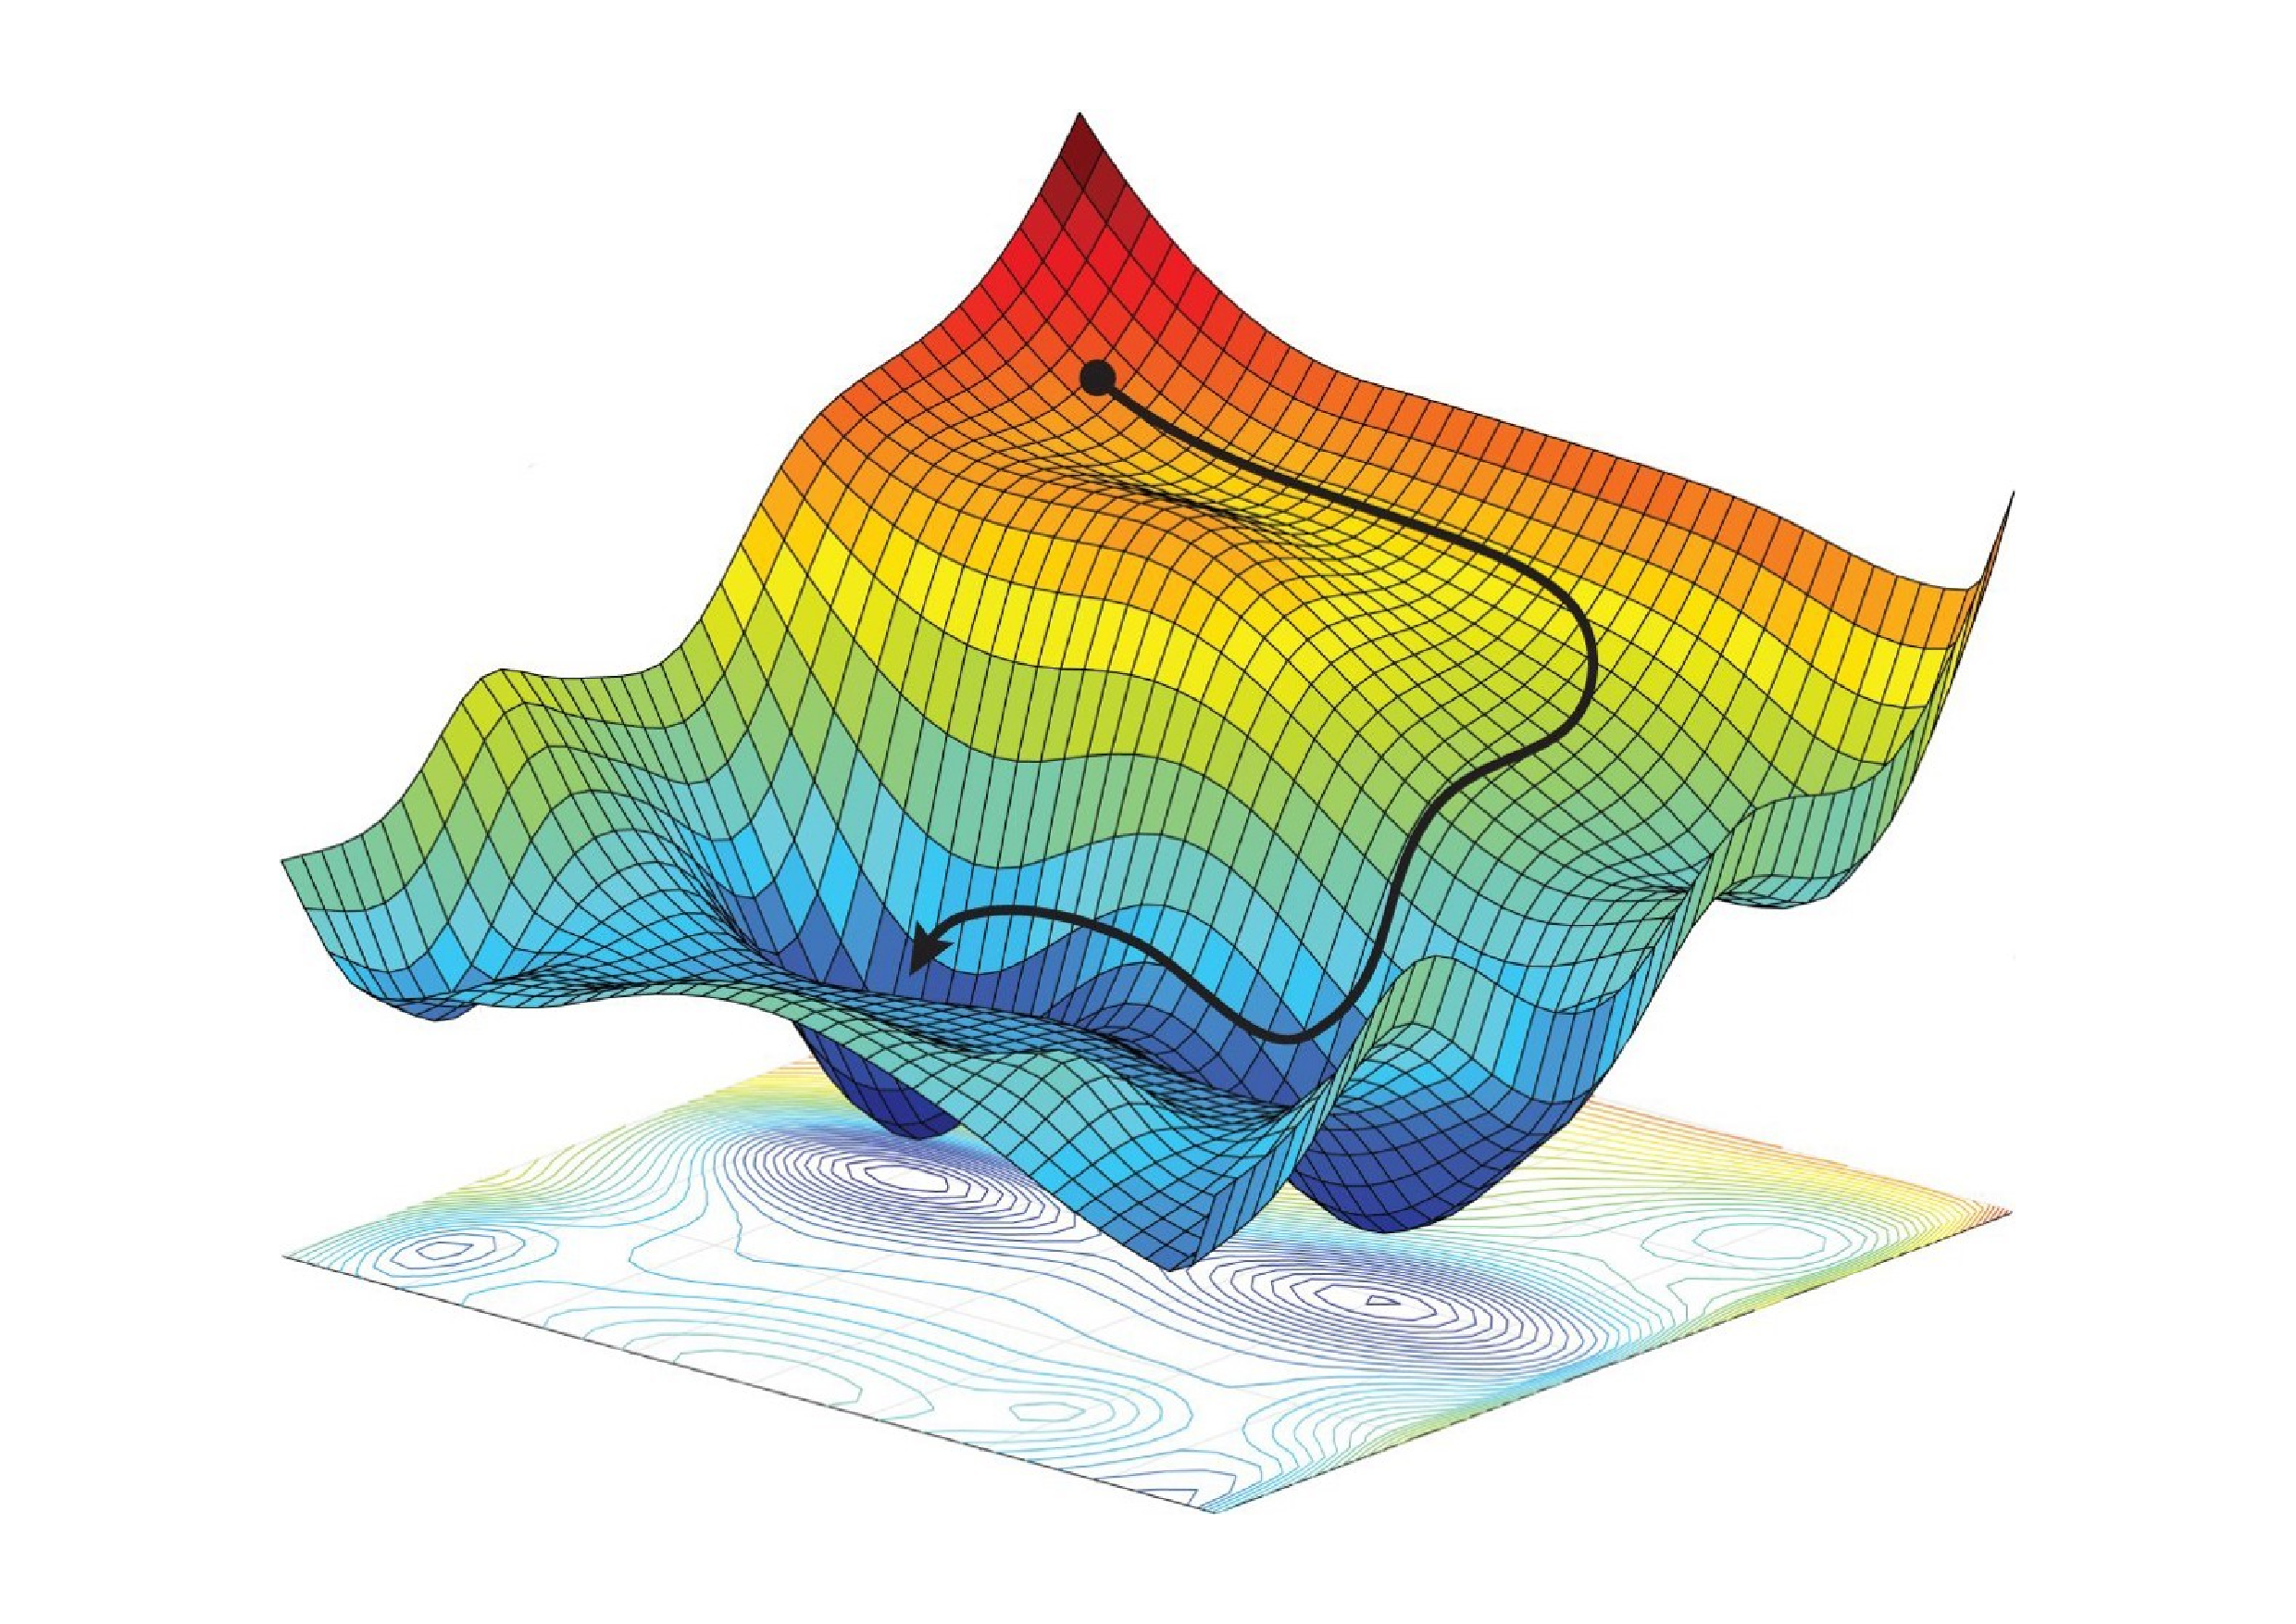
\includegraphics[width=0.7\textwidth]{./Images/gradient_descent.pdf}
    \caption{Representation of the gradient descent method}
    \label{fig:gradient_descent}
\end{figure}

To be honest, \Cref{eq:gradient_descent} does not really tell us how each parameter has to be updated. This job is carried out by \emph{backpropagation} \cite{backprop}, which is based on the \emph{chain rule}. Basically, through backpropagation we can find out how every single parameter needs to change in order to get the aimed gradient descent.

\section{Loss Function}
\label{sec:loss}

In this section we introduce and explain the most common loss functions, also known as \emph{cost functions} or \emph{objectives}.
As we have seen in the previous section, the role of the loss function is to give the neural network a feedback in order for it to be able to learn and improve its accuracy.
In particular, the loss function will return a high value if the actual outcome is far from the expected one and, vice versa, a low value if the outcome matches the correct class.

The first loss function we introduce is the \emph{Multiclass Support Vector Machine loss} (SVM) or \emph{Hinge loss}.
It is based on the concept that we want the neuron in the output layer corresponding to the correct class to have a higher score than the others.
In particular, we want its score to be higher than the wrong neurons by a certain real value called $\Delta$.
If we are evaluating a certain input $\textbf{x}_i$, whose correct class is $y_i$, we can easily implement the SVM loss as
\begin{equation}
    L_i = \sum_{j \neq y_i} \max \left(0, s_j - s_{y_{i}} + \Delta \right)
    \label{eq:SVM}
\end{equation}
where $s_{y_{i}}$ and $s_j$ are respectively the score of the correct class and the score of the other classes. In this way, the loss function will be zero only if the score of the correct class $s_{y_{i}}$ is higher than all the other scores by at least $\Delta$.



\tikzset{every picture/.style={line width=0.75pt}} %set default line width to 0.75pt        

\begin{figure}[h]
    \centering
    \begin{tikzpicture}[x=0.75pt,y=0.75pt,yscale=-1,xscale=1]
%uncomment if require: \path (0,300); %set diagram left start at 0, and has height of 300

%Shape: Boxed Line [id:dp02655229773899892] 
\draw    (90,120) -- (428,120) ;
\draw [shift={(430,120)}, rotate = 180] [color={rgb, 255:red, 0; green, 0; blue, 0 }  ][line width=0.75]    (10.93,-3.29) .. controls (6.95,-1.4) and (3.31,-0.3) .. (0,0) .. controls (3.31,0.3) and (6.95,1.4) .. (10.93,3.29)   ;
%Straight Lines [id:da5317792586208849] 
\draw [color={rgb, 255:red, 65; green, 117; blue, 5 }  ,draw opacity=1 ][line width=2.25]    (120,110) -- (120,130) ;
%Straight Lines [id:da5354681895379683] 
\draw [color={rgb, 255:red, 65; green, 117; blue, 5 }  ,draw opacity=1 ][line width=2.25]    (140,110) -- (140,130) ;
%Straight Lines [id:da5388154142603567] 
\draw [color={rgb, 255:red, 65; green, 117; blue, 5 }  ,draw opacity=1 ][line width=2.25]    (160,110) -- (160,130) ;
%Straight Lines [id:da42918439994677016] 
\draw [color={rgb, 255:red, 65; green, 117; blue, 5 }  ,draw opacity=1 ][line width=2.25]    (180,110) -- (180,130) ;
%Straight Lines [id:da04852367937617719] 
\draw [color={rgb, 255:red, 65; green, 117; blue, 5 }  ,draw opacity=1 ][line width=2.25]    (200,110) -- (200,130) ;
%Straight Lines [id:da8840050377942161] 
\draw [color={rgb, 255:red, 65; green, 117; blue, 5 }  ,draw opacity=1 ][line width=2.25]    (210,110) -- (210,130) ;
%Straight Lines [id:da2574450871983365] 
\draw [color={rgb, 255:red, 208; green, 2; blue, 27 }  ,draw opacity=1 ][line width=1.5]    (230,120) -- (340,120) ;
%Shape: Rectangle [id:dp3877090689212328] 
\draw  [color={rgb, 255:red, 208; green, 2; blue, 27 }  ,draw opacity=1 ][fill={rgb, 255:red, 208; green, 2; blue, 27 }  ,fill opacity=1 ] (225,115) -- (235,115) -- (235,125) -- (225,125) -- cycle ;
%Shape: Rectangle [id:dp21420743746509974] 
\draw  [color={rgb, 255:red, 208; green, 2; blue, 27 }  ,draw opacity=1 ][fill={rgb, 255:red, 208; green, 2; blue, 27 }  ,fill opacity=1 ] (335,115) -- (345,115) -- (345,125) -- (335,125) -- cycle ;
%Straight Lines [id:da9591471900350681] 
\draw [color={rgb, 255:red, 74; green, 144; blue, 226 }  ,draw opacity=1 ][line width=2.25]    (350,110) -- (350,130) ;

% Text Node
\draw (381,102) node [anchor=north west][inner sep=0.75pt]   [align=left] {{\fontfamily{pcr}\selectfont score}};
% Text Node
\draw (350,133) node [anchor=north] [inner sep=0.75pt]  [color={rgb, 255:red, 74; green, 144; blue, 226 }  ,opacity=1 ] [align=left] {$\displaystyle s_{y}{}_{i}$};
% Text Node
\draw (285,123) node [anchor=north] [inner sep=0.75pt]  [color={rgb, 255:red, 208; green, 2; blue, 27 }  ,opacity=1 ] [align=left] {$\displaystyle \Delta $};
% Text Node
\draw (120,133) node [anchor=north] [inner sep=0.75pt]  [color={rgb, 255:red, 65; green, 117; blue, 5 }  ,opacity=1 ] [align=left] {$\displaystyle s_{1}$};
% Text Node
\draw (140,133) node [anchor=north] [inner sep=0.75pt]  [color={rgb, 255:red, 65; green, 117; blue, 5 }  ,opacity=1 ] [align=left] {$\displaystyle s_{2}$};
% Text Node
\draw (180,133) node [anchor=north] [inner sep=0.75pt]  [color={rgb, 255:red, 65; green, 117; blue, 5 }  ,opacity=1 ] [align=left] {$\displaystyle ...$};
% Text Node
\draw (210,133) node [anchor=north] [inner sep=0.75pt]  [color={rgb, 255:red, 65; green, 117; blue, 5 }  ,opacity=1 ] [align=left] {$\displaystyle s_{j}$};


\end{tikzpicture}
    \caption{Representation of how SVM computes the loss}
    \label{fig:SVM}
\end{figure}

A little drawback of the SVM loss is that the set of parameters $W$ is not unique. For instance, if the loss is already zero, any multiple of the set of parameters will also give zero loss. In order to avoid this behaviour, a \emph{regularization penalty $R \left( W \right)$} is added to the SVM loss. A common way to implement the SVM loss is to evaluate it on all the data in parallel and then compute the mean. Thus, the Multiclass SVM loss becomes

\begin{equation}
    L = \frac{1}{N}\sum_i^N L_i + \lambda \sum_k \sum_l W_{k,l}^2
    \label{eq:loss_mean}
\end{equation}

where $N$ is the number of training examples and $\lambda$ is a hyperparameter.

Another popular choice for the loss function is the \emph{cross-entropy loss}, which instead treats the class scores $s_{y_i}$ and $s_j$ as unnormalized log probabilities. Therefore, the \emph{softmax function}, as shown below, returns the probability for the content of the image $\textbf{x}_i$ to be assigned to the correct class $y_i$ according to the current set of parameters $W$

\begin{equation}
   P \left(y_i |\textbf{x}_i; W \right) = \frac{e^{s_{y_{i}}}}{\sum_j e^{s_j}}
   \label{eq:softmax_func}
\end{equation}

The cross-entropy loss has the form

\begin{equation}
     L_i = -\log \left( \frac{e^{s_{y_{i}}}}{\sum_j e^{s_j}} \right)
\end{equation}

and can be interpreted as the negative log likelihood of the correct class. The full loss for the dataset is computed through \Cref{eq:loss_mean}. Minimizing the cross-entropy function means performing the Maximum Likelihood Estimation on the parameters $W$, that is looking for the set of parameters that will maximize the probability on the correct class. 

\section{Neural Networks and Human Brain}
\label{sec:NN_thinking}

We conclude this first chapter with a quick parenthesis on a popular misconception about neural networks.
In fact, often in the media is stated that modern deep learning machines ``think'' or are able to act in a sentient manner. 
Even though it is true that these algorithms are impressive, because of their skills to learn and often succeed in beating the human brain in some restricted fields, it is necessary to understand the differences between thinking and the ability to complete a particular task.

\begin{figure}[h]
    \centering
    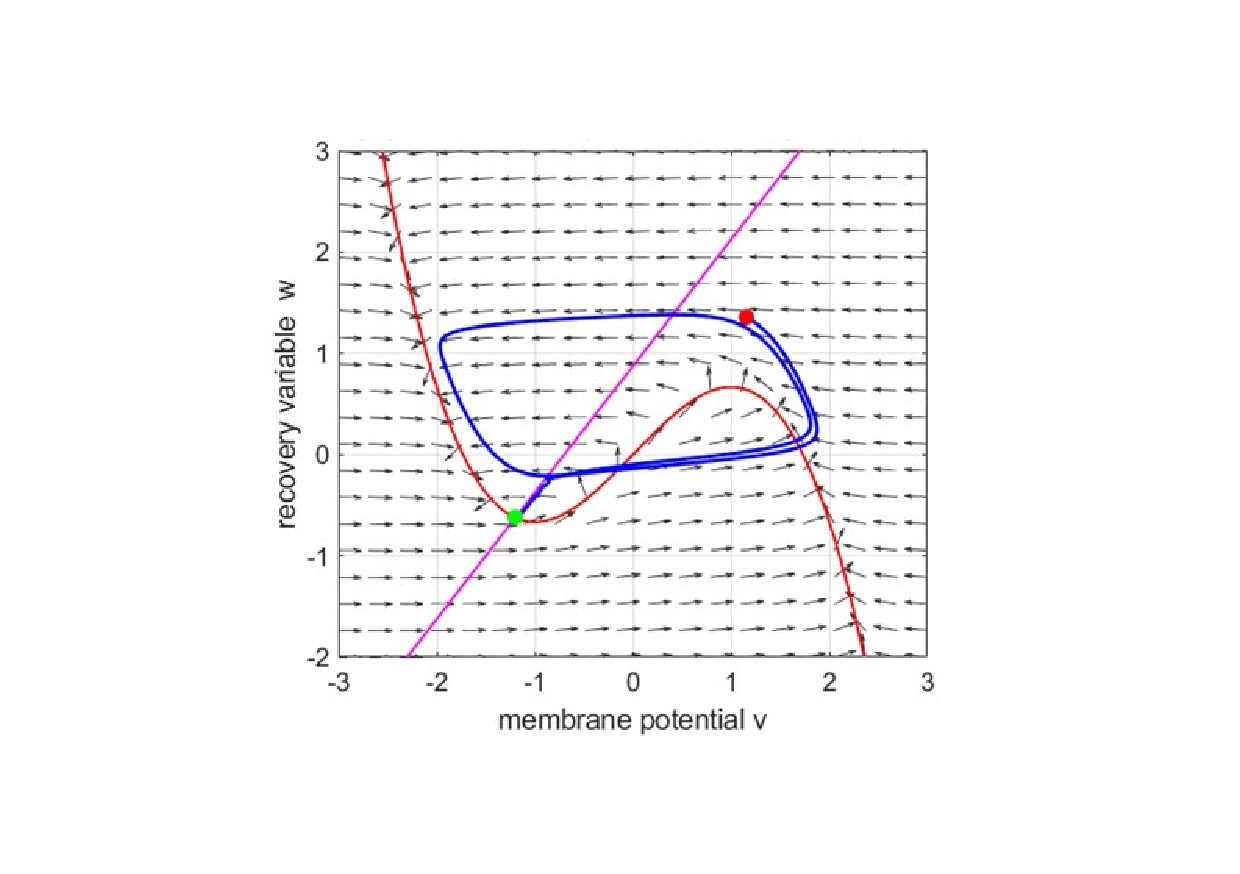
\includegraphics[width=0.5\linewidth, trim={4.5cm 2.3cm 5.2cm 2.3cm}, clip,]{./Images/Fitzhugh-nagumo.pdf}
    \caption{FitzHugh-Nagumo model behaviour}
    \label{fig:Fitzhugh-nagumo}
\end{figure}
Despite the complexity and the extraordinary number of parameters that constitutes modern neural networks, they are just a very simplified model of the human brain.
In fact, we have over 100 billion neurons in our brains connected with more than 100 trillion synapses.
Besides the substantial quantitative difference, also a single biological neuron overcomes the mathematical model in terms of complexity.
Even if simulating the firing of the neuron through a linear product followed by an activation function works well when building an artificial neural network, our real neurons behave in a much more complicated and sophisticated way.
A popular and definitely more realistic model simulating the firing of a neuron is the FitzHugh-Nagumo model, that describes a prototype of an excitable system through two differential equations, whose trend is illustrated in \Cref{fig:Fitzhugh-nagumo}:

\begin{equation}
    \begin{cases}
    \dot{v} = v - \frac{v^3}{3} - w + RI_{ext} \\
    \tau \dot{w} = v + a - b w
    \end{cases}.
    \label{eq:fitzhugh-nagumo}
\end{equation}
In addition, our actual neurons are connected to each other in all sort of arrangements, certainly they are not lined up and sorted to form organised layers as in ANNs.

%\begin{wrapfigure}{l}{0.45\textwidth}
%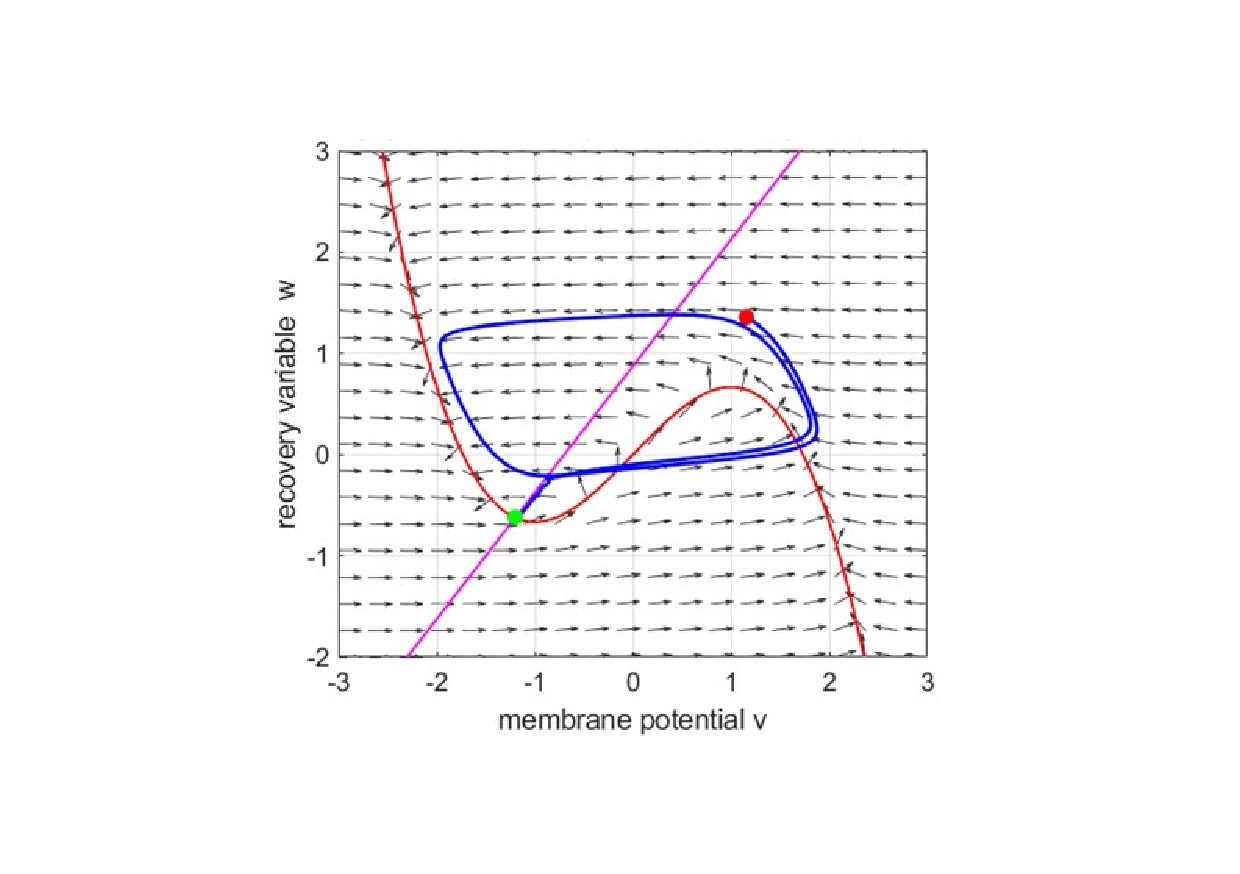
\includegraphics[width=0.9\linewidth, trim={4.5cm 2.3cm 5.2cm 2.3cm}, clip,]{./Images/Fitzhugh-nagumo.pdf}
%\caption{FitzHugh-Nagumo model behaviour}
%\label{fig:Fitzhugh-nagumo}
%\end{wrapfigure}

Despite these facts, often when it comes to learn and perform well in a specific task, artificial neural networks can beat the human brain. But we have to be careful to suggest that deep learning machines have the ability to think.
The reason is because they are not able to take what they learn and apply it to any other problem. Therefore, despite the fact that ``thought'' is something that we do not fully understand, I believe it is clear that learning machines do not actually think (yet).


\chapter{Graphs}
\label{cap:graphs}

In this chapter we define the concept of graph and some matrices associated with it. We study how such matrices reflects some algebraic and topological properties of the graph. We are going to focus in particular on the Laplacian matrix since it plays a key role in spectral graph theory. In the end, we will see some applications of these methods.

\section{Graphs}
\label{sec:graphs}

Let us start from the definition of a graph. There are many real-life examples and applications of graphs, from social networks and protein interactions, to communication networks.
\begin{figure}[ht]
    \centering
    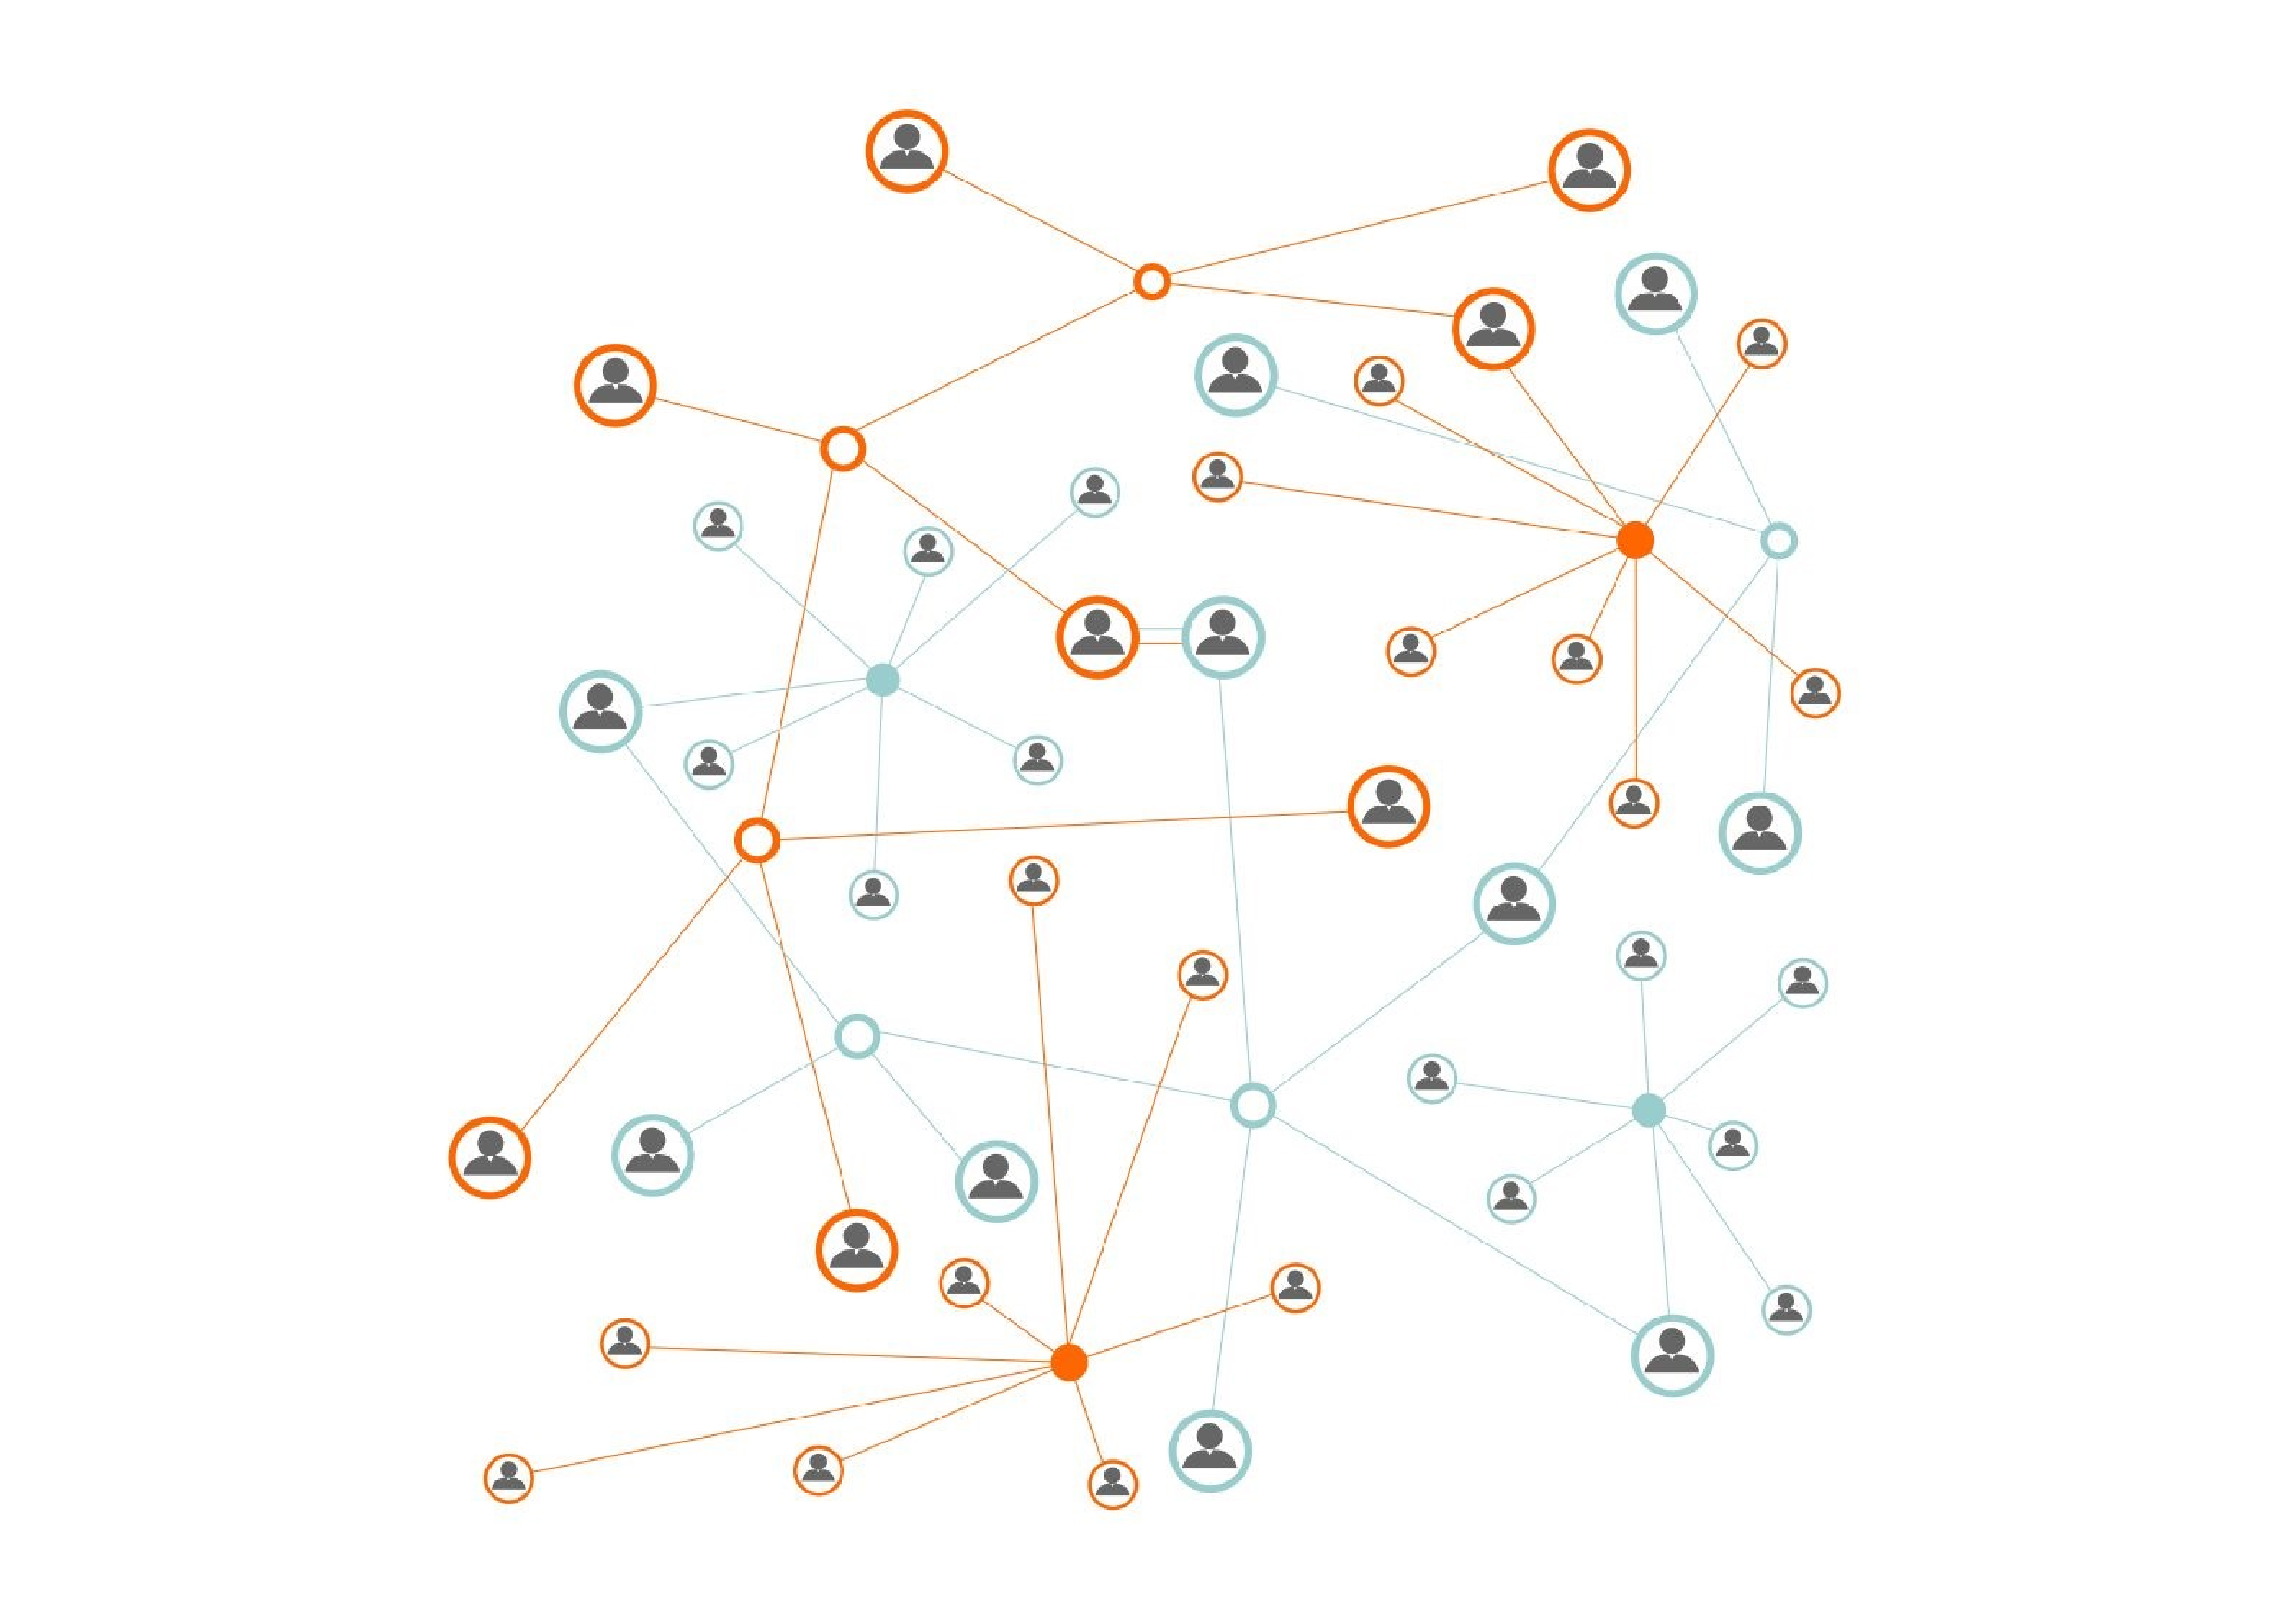
\includegraphics[width=0.5\textwidth, trim={6cm 1.5cm 6cm 1.5cm}, clip]{Images/social_network.pdf}
    \caption{Social network}
    \label{fig:social_network}
\end{figure}
\begin{definition}
A \emph{graph} $\mathcal{G}$ is a pair of sets $(\mathcal{V}, \mathcal{E})$, where $\mathcal{V} = \{1, \ldots, n\}$ and $\mathcal{E} \subseteq \mathcal{V} \times \mathcal{V}$. The elements of $\mathcal{V}$ are called nodes or vertices. The elements of $\mathcal{E}$ are called edges.
\end{definition}
The nodes of a graph can be labelled as $v_1, \ldots, v_n$.
The edges can be also numbered and referred to with $e_1, \ldots, e_k$, where $k$ indicates the number of edges, or can be labelled in order to show the two nodes that they connect;
for example, if an edge links node $v_i$ and $v_j$, we label it with $e_{ij}$.

A graph can be \emph{undirected} if the edges do not have a direction, therefore if $v_i$ is connected to $v_j$, $v_j$ is connected to $v_i$ as well; otherwise the graph is called \emph{directed}.

\begin{figure}[h]
\centering
\begin{subfigure}{.5\textwidth}
  \centering
        \begin{tikzpicture}[x=0.75pt,y=0.75pt,yscale=-1,xscale=1]
    %uncomment if require: \path (0,355); %set diagram left start at 0, and has height of 355
    
    %Shape: Circle [id:dp20198698366856682] 
    \draw   (227.57,133.46) .. controls (231.18,137.64) and (230.72,143.96) .. (226.54,147.57) .. controls (222.36,151.18) and (216.04,150.72) .. (212.43,146.54) .. controls (208.82,142.36) and (209.28,136.04) .. (213.46,132.43) .. controls (217.64,128.82) and (223.96,129.28) .. (227.57,133.46) -- cycle ;
    %Shape: Circle [id:dp7969044060319974] 
    \draw   (187.97,180.21) .. controls (193.37,179.09) and (198.67,182.56) .. (199.79,187.97) .. controls (200.91,193.37) and (197.44,198.67) .. (192.03,199.79) .. controls (186.63,200.91) and (181.33,197.44) .. (180.21,192.03) .. controls (179.09,186.63) and (182.56,181.33) .. (187.97,180.21) -- cycle ;
    %Shape: Circle [id:dp7464547325669635] 
    \draw   (261.48,189.89) .. controls (256.02,190.71) and (250.93,186.95) .. (250.11,181.48) .. controls (249.29,176.02) and (253.05,170.93) .. (258.52,170.11) .. controls (263.98,169.29) and (269.07,173.05) .. (269.89,178.52) .. controls (270.71,183.98) and (266.95,189.07) .. (261.48,189.89) -- cycle ;
    %Shape: Circle [id:dp6985974571194418] 
    \draw   (315.7,158.21) .. controls (311.17,161.36) and (304.94,160.24) .. (301.79,155.7) .. controls (298.64,151.17) and (299.76,144.94) .. (304.3,141.79) .. controls (308.83,138.64) and (315.06,139.76) .. (318.21,144.3) .. controls (321.36,148.83) and (320.24,155.06) .. (315.7,158.21) -- cycle ;
    %Straight Lines [id:da8290134642544309] 
    \draw    (194.69,181.17) -- (214.85,148.57) ;
    %Straight Lines [id:da4300652277419019] 
    \draw    (226.54,147.57) -- (252.46,173.43) ;
    %Straight Lines [id:da9290753477048785] 
    \draw    (268.52,174.77) -- (301.79,155.7) ;
    %Straight Lines [id:da672574792362391] 
    \draw    (199.79,187.97) -- (250.11,181.48) ;
    
    % Text Node
    \draw (215.46,133.43) node [anchor=north west][inner sep=0.75pt]  [font=\footnotesize] [align=left] {$\displaystyle 1$};
    % Text Node
    \draw (186,183) node [anchor=north west][inner sep=0.75pt]  [font=\footnotesize] [align=left] {$\displaystyle 2$};
    % Text Node
    \draw (256,173) node [anchor=north west][inner sep=0.75pt]  [font=\footnotesize] [align=left] {$\displaystyle 3$};
    % Text Node
    \draw (305,143) node [anchor=north west][inner sep=0.75pt]  [font=\footnotesize] [align=left] {$\displaystyle 4$};
    
    
    \end{tikzpicture}
  \caption{Undirected graph}
  \label{fig:undirected_graph}
\end{subfigure}%
\begin{subfigure}{.5\textwidth}
  \centering
        \begin{tikzpicture}[x=0.75pt,y=0.75pt,yscale=-1,xscale=1]
    %uncomment if require: \path (0,355); %set diagram left start at 0, and has height of 355
    
    %Shape: Circle [id:dp20198698366856682] 
    \draw   (227.57,133.46) .. controls (231.18,137.64) and (230.72,143.96) .. (226.54,147.57) .. controls (222.36,151.18) and (216.04,150.72) .. (212.43,146.54) .. controls (208.82,142.36) and (209.28,136.04) .. (213.46,132.43) .. controls (217.64,128.82) and (223.96,129.28) .. (227.57,133.46) -- cycle ;
    %Shape: Circle [id:dp7969044060319974] 
    \draw   (187.97,180.21) .. controls (193.37,179.09) and (198.67,182.56) .. (199.79,187.97) .. controls (200.91,193.37) and (197.44,198.67) .. (192.03,199.79) .. controls (186.63,200.91) and (181.33,197.44) .. (180.21,192.03) .. controls (179.09,186.63) and (182.56,181.33) .. (187.97,180.21) -- cycle ;
    %Shape: Circle [id:dp7464547325669635] 
    \draw   (261.48,189.89) .. controls (256.02,190.71) and (250.93,186.95) .. (250.11,181.48) .. controls (249.29,176.02) and (253.05,170.93) .. (258.52,170.11) .. controls (263.98,169.29) and (269.07,173.05) .. (269.89,178.52) .. controls (270.71,183.98) and (266.95,189.07) .. (261.48,189.89) -- cycle ;
    %Shape: Circle [id:dp6985974571194418] 
    \draw   (315.7,158.21) .. controls (311.17,161.36) and (304.94,160.24) .. (301.79,155.7) .. controls (298.64,151.17) and (299.76,144.94) .. (304.3,141.79) .. controls (308.83,138.64) and (315.06,139.76) .. (318.21,144.3) .. controls (321.36,148.83) and (320.24,155.06) .. (315.7,158.21) -- cycle ;
    %Straight Lines [id:da5254460671370087] 
    \draw    (214.85,148.57) -- (195.75,179.47) ;
    \draw [shift={(194.69,181.17)}, rotate = 301.73] [color={rgb, 255:red, 0; green, 0; blue, 0 }  ][line width=0.75]    (10.93,-3.29) .. controls (6.95,-1.4) and (3.31,-0.3) .. (0,0) .. controls (3.31,0.3) and (6.95,1.4) .. (10.93,3.29)   ;
    %Straight Lines [id:da09600700402219187] 
    \draw    (301.79,155.7) -- (270.26,173.77) ;
    \draw [shift={(268.52,174.77)}, rotate = 330.18] [color={rgb, 255:red, 0; green, 0; blue, 0 }  ][line width=0.75]    (10.93,-3.29) .. controls (6.95,-1.4) and (3.31,-0.3) .. (0,0) .. controls (3.31,0.3) and (6.95,1.4) .. (10.93,3.29)   ;
    %Straight Lines [id:da9692198996776262] 
    \draw    (226.54,147.57) -- (251.05,172.02) ;
    \draw [shift={(252.46,173.43)}, rotate = 224.93] [color={rgb, 255:red, 0; green, 0; blue, 0 }  ][line width=0.75]    (10.93,-3.29) .. controls (6.95,-1.4) and (3.31,-0.3) .. (0,0) .. controls (3.31,0.3) and (6.95,1.4) .. (10.93,3.29)   ;
    %Straight Lines [id:da5253861982309282] 
    \draw    (250.11,181.48) -- (201.97,189.66) ;
    \draw [shift={(200,190)}, rotate = 350.36] [color={rgb, 255:red, 0; green, 0; blue, 0 }  ][line width=0.75]    (10.93,-3.29) .. controls (6.95,-1.4) and (3.31,-0.3) .. (0,0) .. controls (3.31,0.3) and (6.95,1.4) .. (10.93,3.29)   ;
    
    % Text Node
    \draw (215.46,133.43) node [anchor=north west][inner sep=0.75pt]  [font=\footnotesize] [align=left] {$\displaystyle 1$};
    % Text Node
    \draw (186,183) node [anchor=north west][inner sep=0.75pt]  [font=\footnotesize] [align=left] {$\displaystyle 2$};
    % Text Node
    \draw (256,173) node [anchor=north west][inner sep=0.75pt]  [font=\footnotesize] [align=left] {$\displaystyle 3$};
    % Text Node
    \draw (305,143) node [anchor=north west][inner sep=0.75pt]  [font=\footnotesize] [align=left] {$\displaystyle 4$};
    
    
    \end{tikzpicture}
  \caption{Directed graph}
  \label{fig:directed_graph}
\end{subfigure}
\caption{Graph examples}
\label{fig:graph_examples}
\end{figure}

A way to represent the connections and the topological structure of a graph is through the adjacency matrix.
\begin{definition}
The \emph{adjacency matrix $A$} of a graph $\mathcal{G}$ is a $|\mathcal{V}| \times |\mathcal{V}|$ matrix and can be defined as
\begin{equation*}
    A_{ij} = 
    \begin{cases}
    1 & e_{ij} \in \mathcal{E} \\
    0 & \text{otherwise}
    \end{cases}.
\end{equation*}
\end{definition}
It is easy to understand that in a undirected graph $A_{ij}=1$ if and only if $A_{ji}=1$, since $e_{ij} \in \mathcal{E}$ if and only if $e_{ji} \in \mathcal{E}$, hence $A$ is a symmetric matrix.
Let us see the adjacency matrices for the simple graphs shown in \Cref{fig:graph_examples}.
\begin{figure}[h]
\begin{minipage}[b]{0.45\linewidth}
\centering
    \begin{equation*}
    A = 
    \begin{pmatrix}
    0 & 1 & 1 & 0 \\
    1 & 0 & 1 & 0 \\
    1 & 1 & 0 & 1 \\
    0 & 0 & 1 & 0 
    \end{pmatrix}
    \end{equation*}
\caption{Adjacency matrix for the undirected graph in \Cref{fig:undirected_graph}}
\label{fig:A_undirected}
\end{minipage}
\hspace{0.5cm}
\begin{minipage}[b]{0.45\linewidth}
\centering
    \begin{equation*}
    A = 
    \begin{pmatrix}
    0 & 1 & 1 & 0 \\
    0 & 0 & 0 & 0 \\
    0 & 1 & 0 & 0 \\
    0 & 0 & 1 & 0 
    \end{pmatrix}
    \end{equation*}
\caption{Adjacency matrix for the directed graph in \Cref{fig:directed_graph}}
\label{fig:A_directed}
\end{minipage}
\end{figure}

In addition, a graph can also have weights associated with its edges, in this case the adjacency matrix is more commonly denoted with $W$ and called weight matrix.
\begin{definition}
The \emph{weight matrix $W$} of a graph $\mathcal{G}$ is a $|\mathcal{V}| \times |\mathcal{V}|$ matrix, where $W_{ij}$ is the weight of the edge $e_{ij}$. If $e_{ij} \notin \mathcal{E}$, then $W_{ij} = 0$.
\end{definition}

We define the \emph{node degree} as the number of edges connected with a particular vertex.
In the graph of \Cref{fig:undirected_graph}, for example, the degree of the first node is 2, and we write this as $\deg(v_1)=2$.
In a directed graph, instead, we have the \emph{indegree} and the \emph{outdegree}, being, respectively, the number of edges leading into that node and those leading away from it.
If $\deg(v)=k$ for every node $v$, then we call the graph \emph{regular}.
We now introduce the concept of degree matrix.
\begin{definition}
The \emph{degree matrix $D$} of an undirected graph $\mathcal{G}$ is a $|\mathcal{V}| \times |\mathcal{V}|$ diagonal matrix displaying the degree of each node on its diagonal, namely $D_{ii} = \deg(v_i).$
\end{definition}

We refer to the set of vertices adjacent with a node $v_i$ as the \emph{neighbourhood $\mathcal{N}\left( v_i \right)$} of the vertex $v_i$.

Let us now introduce and discuss briefly an interesting theorem.
\begin{theorem}
\label{the:walks}
Let $\mathcal{G}$ be a graph and $A$ its adjacency matrix, then $\left( A^r \right)_{ij}$ represents the number of walks of length $r$ from $v_i$ to $v_j$.
\end{theorem}
Before the proof we look at a simple example.
\begin{example}
We look at $A^2$ for a simple graph, like the undirected graph in \Cref{fig:undirected_graph}, that for convenience it is reported below.
\begin{figure}[h]
\centering
    \begin{minipage}[]{0.3\linewidth}
    \centering
        \begin{equation*}
        A^2 =
        \begin{pmatrix}
        2 & 1 & 1 & 1 \\
        1 & 2 & 1 & 1 \\
        \textcolor{tikz_blue}{1} & \textcolor{tikz_green}{1} & \textcolor{tikz_red}{3} & 0 \\
        1 & 1 & 0 & 1
        \end{pmatrix}
        \end{equation*}
    \label{fig:A^2}
    \end{minipage}
\hspace{1cm}
    \begin{minipage}[]{0.3\linewidth}
    \centering
        \begin{tikzpicture}[x=0.75pt,y=0.75pt,yscale=-1,xscale=1]
        %uncomment if require: \path (0,355); %set diagram left start at 0, and has height of 355
        
        %Shape: Circle [id:dp20198698366856682] 
        \draw   (227.57,133.46) .. controls (231.18,137.64) and (230.72,143.96) .. (226.54,147.57) .. controls (222.36,151.18) and (216.04,150.72) .. (212.43,146.54) .. controls (208.82,142.36) and (209.28,136.04) .. (213.46,132.43) .. controls (217.64,128.82) and (223.96,129.28) .. (227.57,133.46) -- cycle ;
        %Shape: Circle [id:dp7969044060319974] 
        \draw   (187.97,180.21) .. controls (193.37,179.09) and (198.67,182.56) .. (199.79,187.97) .. controls (200.91,193.37) and (197.44,198.67) .. (192.03,199.79) .. controls (186.63,200.91) and (181.33,197.44) .. (180.21,192.03) .. controls (179.09,186.63) and (182.56,181.33) .. (187.97,180.21) -- cycle ;
        %Shape: Circle [id:dp7464547325669635] 
        \draw   (261.48,189.89) .. controls (256.02,190.71) and (250.93,186.95) .. (250.11,181.48) .. controls (249.29,176.02) and (253.05,170.93) .. (258.52,170.11) .. controls (263.98,169.29) and (269.07,173.05) .. (269.89,178.52) .. controls (270.71,183.98) and (266.95,189.07) .. (261.48,189.89) -- cycle ;
        %Shape: Circle [id:dp6985974571194418] 
        \draw   (315.7,158.21) .. controls (311.17,161.36) and (304.94,160.24) .. (301.79,155.7) .. controls (298.64,151.17) and (299.76,144.94) .. (304.3,141.79) .. controls (308.83,138.64) and (315.06,139.76) .. (318.21,144.3) .. controls (321.36,148.83) and (320.24,155.06) .. (315.7,158.21) -- cycle ;
        %Straight Lines [id:da8290134642544309] 
        \draw    (194.69,181.17) -- (214.85,148.57) ;
        %Straight Lines [id:da4300652277419019] 
        \draw    (226.54,147.57) -- (252.46,173.43) ;
        %Straight Lines [id:da9290753477048785] 
        \draw    (268.52,174.77) -- (301.79,155.7) ;
        %Straight Lines [id:da672574792362391] 
        \draw    (199.79,187.97) -- (250.11,181.48) ;
        %Curve Lines [id:da6685644991335284] 
        \draw [color={rgb, 255:red, 208; green, 2; blue, 27 }  ,draw opacity=1 ]   (255,171) .. controls (249.43,160.44) and (241.64,152.4) .. (230.58,145.91) ;
        \draw [shift={(229,145)}, rotate = 29.2] [color={rgb, 255:red, 208; green, 2; blue, 27 }  ,draw opacity=1 ][line width=0.75]    (10.93,-3.29) .. controls (6.95,-1.4) and (3.31,-0.3) .. (0,0) .. controls (3.31,0.3) and (6.95,1.4) .. (10.93,3.29)   ;
        %Curve Lines [id:da7919998543240745] 
        \draw [color={rgb, 255:red, 208; green, 2; blue, 27 }  ,draw opacity=1 ]   (225,149) .. controls (232.49,160.48) and (239.05,167.5) .. (249.34,173.98) ;
        \draw [shift={(251,175)}, rotate = 211.03] [color={rgb, 255:red, 208; green, 2; blue, 27 }  ,draw opacity=1 ][line width=0.75]    (10.93,-3.29) .. controls (6.95,-1.4) and (3.31,-0.3) .. (0,0) .. controls (3.31,0.3) and (6.95,1.4) .. (10.93,3.29)   ;
        %Curve Lines [id:da8634657487949378] 
        \draw [color={rgb, 255:red, 208; green, 2; blue, 27 }  ,draw opacity=1 ]   (266,172) .. controls (274.62,161.47) and (288.52,155.79) .. (298.2,152.58) ;
        \draw [shift={(300,152)}, rotate = 162.33] [color={rgb, 255:red, 208; green, 2; blue, 27 }  ,draw opacity=1 ][line width=0.75]    (10.93,-3.29) .. controls (6.95,-1.4) and (3.31,-0.3) .. (0,0) .. controls (3.31,0.3) and (6.95,1.4) .. (10.93,3.29)   ;
        %Curve Lines [id:da059205098908762244] 
        \draw [color={rgb, 255:red, 208; green, 2; blue, 27 }  ,draw opacity=1 ]   (306,160) .. controls (300.54,166.25) and (285.58,174.67) .. (271.73,179.42) ;
        \draw [shift={(270,180)}, rotate = 342.08] [color={rgb, 255:red, 208; green, 2; blue, 27 }  ,draw opacity=1 ][line width=0.75]    (10.93,-3.29) .. controls (6.95,-1.4) and (3.31,-0.3) .. (0,0) .. controls (3.31,0.3) and (6.95,1.4) .. (10.93,3.29)   ;
        %Curve Lines [id:da7244655796355257] 
        \draw [color={rgb, 255:red, 208; green, 2; blue, 27 }  ,draw opacity=1 ]   (250,179) .. controls (235.6,177.08) and (216.22,179.77) .. (201.78,184.41) ;
        \draw [shift={(200,185)}, rotate = 341.1] [color={rgb, 255:red, 208; green, 2; blue, 27 }  ,draw opacity=1 ][line width=0.75]    (10.93,-3.29) .. controls (6.95,-1.4) and (3.31,-0.3) .. (0,0) .. controls (3.31,0.3) and (6.95,1.4) .. (10.93,3.29)   ;
        %Curve Lines [id:da27298212293137336] 
        \draw [color={rgb, 255:red, 208; green, 2; blue, 27 }  ,draw opacity=1 ]   (200,192) .. controls (215.23,194.63) and (238.33,188.86) .. (249.1,185.59) ;
        \draw [shift={(251,185)}, rotate = 162.33] [color={rgb, 255:red, 208; green, 2; blue, 27 }  ,draw opacity=1 ][line width=0.75]    (10.93,-3.29) .. controls (6.95,-1.4) and (3.31,-0.3) .. (0,0) .. controls (3.31,0.3) and (6.95,1.4) .. (10.93,3.29)   ;
        %Curve Lines [id:da5523815849568599] 
        \draw [color={rgb, 255:red, 126; green, 211; blue, 33 }  ,draw opacity=1 ]   (250,177) .. controls (237.48,176.73) and (232.61,172.54) .. (222.77,151.64) ;
        \draw [shift={(222,150)}, rotate = 65.1] [color={rgb, 255:red, 126; green, 211; blue, 33 }  ,draw opacity=1 ][line width=0.75]    (10.93,-3.29) .. controls (6.95,-1.4) and (3.31,-0.3) .. (0,0) .. controls (3.31,0.3) and (6.95,1.4) .. (10.93,3.29)   ;
        %Curve Lines [id:da4597133351326428] 
        \draw [color={rgb, 255:red, 126; green, 211; blue, 33 }  ,draw opacity=1 ]   (220,150) .. controls (218.01,159.28) and (214.92,166.36) .. (198.3,181.8) ;
        \draw [shift={(197,183)}, rotate = 317.49] [color={rgb, 255:red, 126; green, 211; blue, 33 }  ,draw opacity=1 ][line width=0.75]    (10.93,-3.29) .. controls (6.95,-1.4) and (3.31,-0.3) .. (0,0) .. controls (3.31,0.3) and (6.95,1.4) .. (10.93,3.29)   ;
        %Curve Lines [id:da9617927400863351] 
        \draw [color={rgb, 255:red, 74; green, 144; blue, 226 }  ,draw opacity=1 ]   (260,190) .. controls (225.04,206.99) and (209.31,206.75) .. (191.65,200.59) ;
        \draw [shift={(190,200)}, rotate = 20.1] [color={rgb, 255:red, 74; green, 144; blue, 226 }  ,draw opacity=1 ][line width=0.75]    (10.93,-3.29) .. controls (6.95,-1.4) and (3.31,-0.3) .. (0,0) .. controls (3.31,0.3) and (6.95,1.4) .. (10.93,3.29)   ;
        %Curve Lines [id:da01579637826247371] 
        \draw [color={rgb, 255:red, 74; green, 144; blue, 226 }  ,draw opacity=1 ]   (180,190) .. controls (167.16,173.24) and (193.12,152.04) .. (208.6,140.99) ;
        \draw [shift={(210,140)}, rotate = 144.88] [color={rgb, 255:red, 74; green, 144; blue, 226 }  ,draw opacity=1 ][line width=0.75]    (10.93,-3.29) .. controls (6.95,-1.4) and (3.31,-0.3) .. (0,0) .. controls (3.31,0.3) and (6.95,1.4) .. (10.93,3.29)   ;
        
        % Text Node
        \draw (215.46,133.43) node [anchor=north west][inner sep=0.75pt]  [font=\footnotesize] [align=left] {$\displaystyle 1$};
        % Text Node
        \draw (186,183) node [anchor=north west][inner sep=0.75pt]  [font=\footnotesize] [align=left] {$\displaystyle 2$};
        % Text Node
        \draw (256,173) node [anchor=north west][inner sep=0.75pt]  [font=\footnotesize] [align=left] {$\displaystyle 3$};
        % Text Node
        \draw (305,143) node [anchor=north west][inner sep=0.75pt]  [font=\footnotesize] [align=left] {$\displaystyle 4$};
        
        
        \end{tikzpicture}
    \label{fig:graph^2}
    \end{minipage}
\end{figure}

Let us first focus on the diagonal.
It should appear clear that $\left( A^2 \right)_{ii} = \deg \left( v_i \right)$.
In fact, the number of walks of length 2 starting from $v_i$ and finishing in $v_i$ again is exactly the degree of the node, because the only possible walks are $v_i \rightarrow v_k \rightarrow v_i$ for all $v_k \in \mathcal{N}\left( v_i \right)$.
We can express matrix multiplication as $C_{ij} = \sum_k A_{ik} B_{kj}$. In this way, we can also understand the meaning of the off-diagonal terms.
In fact,
\begin{equation*}
    \left( A^2 \right)_{ij} = \sum_k A_{ik} A_{kj}
\end{equation*}
and the term $A_{ik} A_{kj}$ will bring a contribution to the sum for a particular $k$ only if both $A_{ik}$ and $A_{kj}$ are different from zero, which means that the edges $e_{ik}$ and $e_{kj}$ belong both to $\mathcal{E}$, therefore the walk $v_i \rightarrow v_k \rightarrow v_j$ is allowed. 
\end{example}

We now prove the \Cref{the:walks} by induction.
\begin{proof}
$A^1_{ij}$ clearly represents the number of walks of length $1$ from $v_i$ to $v_j$. Suppose that $\left( A^{(r-1)} \right)_{ik}$ represents the number of walks of length $(r-1)$ from $v_i$ to $v_k$, then
\begin{equation*}
    \left( A^{r} \right)_{ij} = \sum_k \left( A^{r-1} \right)_{ik} A_{kj}.
\end{equation*}
For a particular $\Tilde{k}$, the only way for $\left( A^{r-1} \right)_{i \Tilde{k}} A_{\Tilde{k} j}$ to be different from zero is to have at least $1$ walk of length $(r-1)$ from $v_i$ to $v_{\Tilde{k}}$ and $e_{\Tilde{k} j} \in \mathcal{E}$.
If these conditions are satisfied, then it contributes to the sum over $k$ with $\left( A^{r-1} \right)_{i \Tilde{k}}$ walks from $v_i$ to $v_{\Tilde{k}}$ of length $(r-1)$, followed by a final step from $v_{\Tilde{k}}$ to $v_j$.
Summing over $k$ will sum all these contributions, resulting in the number of walks of length $r$ from $v_i$ to $v_j$.
\end{proof}

\section{Diffusion on graph}
\label{sec:diffusion}

%Let us talk about the problem of finding the eigenvalues and eigenvectors of the adjacency matrix, even though we %will not be interested in the eigenvectors of A in the next sections. We write the usual eigenvalue equation as
%\begin{equation}
%    A \mathbf{x} = \lambda \mathbf{x}
%    \label{eq:eigen_A}
%\end{equation}
%where $\lambda$ is the eigenvalue associated with the eigenvector $\mathbf{x} \in \mathbb{R}^n$. 
Let $\mathbb{R}^{\mathcal{V}}$ denote the real valued functions on the set of vertices $\mathcal{V}$:
\begin{equation*}
    \mathbb{R}^{\mathcal{V}} = \{ f : \mathcal{V} \rightarrow \mathbb{R} \} .
\end{equation*}
If we give an ordering to $\mathcal{V}$, we can identify $\mathbb{R}^{\mathcal{V}}$ with $\mathbb{R}^n$, where $n$ denotes the number of nodes.
This identifies a function in $\mathbb{R}^{\mathcal{V}}$ with a vector in $\mathbb{R}^n$, namely
\begin{equation*}
    \mathbf{f} = \left( f_1 , \ldots , f_n \right) = 
    \left( f(v_1) , \ldots , f(v_n) \right) \in \mathbb{R}^n .
\end{equation*}
This means we can view the adjacency matrix $A$ as a linear mapping on $\mathbb{R}^{\mathcal{V}}$, rather than its isomorphic vector space $\mathbb{R}^n$. As a consequence, we see that 
\begin{equation*}
    \left( A f \right) (u) = \sum_{v \in \mathcal{V}} A_{uv} f(v) = \sum_{v \in \mathcal{N}(u)} f (v) , \quad f \in \mathbb{R}^{\mathcal{V}} .
\end{equation*}
Thus, the value of $Af$ at node $u$ is the sum of the values of $f$ on the neighbours of $u$.
If we now suppose that $x \in \mathbb{R}^{\mathcal{V}}$ is an eigenfunction of $A$, we can write
\begin{equation*}
    \left( A x \right) ( u ) = \lambda x ( u ) \Longrightarrow \sum_{v \in \mathcal{N}(u)} x(v) = \lambda x(u) \quad \forall u \in \mathcal{V}.
\end{equation*}

In words, the sum of the values of the eigenfunction $x$ on the neighbours of node $u$ is $\lambda$ times its value at point $u$ itself.

An important matrix is the \emph{diffusion} or \emph{walk matrix}, defined as $A D^{-1}$. Being $D$ the degree matrix, its inverse will be $D^{-1} = \text{diag}\left(1/\deg(v_1), \ldots, 1/\deg(v_n) \right)$. Thus, if we apply $AD^{-1}$ to a function $f$ in $\mathbb{R}^{\mathcal{V}}$ at a node $u$, it will return
\begin{equation*}
    \left( \left( AD^{-1}\right) f \right) (u) = \sum_{v \in \mathcal{V}} \sum_{k \in \mathcal{V}}  A_{uk} D^{-1}_{kv} f(v) = \sum_{v \in \mathcal{V}} \frac{A_{uv}}{\deg(v)} f(v) = \sum_{v \in \mathcal{N}(u)} \frac{f (v)}{\deg(v)}.
\end{equation*}
We can compare this with a similar but slightly different result that we will need later on, that is applying $D^{-1} A$ to the same function $f$ at node $u$:
\begin{equation*}
    \left( \left( D^{-1} A\right) f \right) (u) = \sum_{k \in \mathcal{V}} \sum_{v \in \mathcal{V}}  D^{-1}_{uk} A_{kv} f(v) = \sum_{v \in \mathcal{V}} \frac{A_{uv}}{\deg(u)} f(v) = \sum_{v \in \mathcal{N}(u)} \frac{f (v)}{\deg(u)}.
\end{equation*}
$\left( (D^{-1} A) f \right)(u)$ gives an average of $f(v)$, with $v$ node in the neighbourhood of $u$.
Both of the results require a sum over the values of function $f$ at the neighbours of the node $u$, the only difference is that in the former we divide each $f(v)$ for the degree of the node $v$, in the latter we normalize the sum with the degree of node $u$.

\section{Incidence Matrix and Gradient}
\label{sec:incidence_gradient}

In this section we introduce the incidence matrix $X$ and its interpretation as the discrete gradient on a graph.
Assume $f$ is a real function on the set of vertices $\mathcal{V}$ as seen before.
\begin{figure}[h]
\begin{minipage}[]{0.45\linewidth}
\begin{align*}
    f \colon \mathcal{V} & \longrightarrow \mathbb{R} \\
    v_i & \longmapsto f(v_i) = f_i .
\end{align*}
\end{minipage}
\hspace{0.5cm}
\begin{minipage}[]{0.45\linewidth}
    \centering
    \resizebox{0.75 \textwidth}{!}{
        \begin{tikzpicture}[x=0.75pt,y=0.75pt,yscale=-1,xscale=1]
%uncomment if require: \path (0,300); %set diagram left start at 0, and has height of 300

%Shape: Ellipse [id:dp037223241543863805] 
\draw   (220,115) .. controls (220,106.72) and (233.43,100) .. (250,100) .. controls (266.57,100) and (280,106.72) .. (280,115) .. controls (280,123.28) and (266.57,130) .. (250,130) .. controls (233.43,130) and (220,123.28) .. (220,115) -- cycle ;
%Shape: Ellipse [id:dp07413277469951374] 
\draw   (300,175) .. controls (300,166.72) and (313.43,160) .. (330,160) .. controls (346.57,160) and (360,166.72) .. (360,175) .. controls (360,183.28) and (346.57,190) .. (330,190) .. controls (313.43,190) and (300,183.28) .. (300,175) -- cycle ;
%Shape: Ellipse [id:dp8686186114444554] 
\draw   (130,195) .. controls (130,186.72) and (143.43,180) .. (160,180) .. controls (176.57,180) and (190,186.72) .. (190,195) .. controls (190,203.28) and (176.57,210) .. (160,210) .. controls (143.43,210) and (130,203.28) .. (130,195) -- cycle ;
%Shape: Ellipse [id:dp4643328529017021] 
\draw   (420,135) .. controls (420,126.72) and (433.43,120) .. (450,120) .. controls (466.57,120) and (480,126.72) .. (480,135) .. controls (480,143.28) and (466.57,150) .. (450,150) .. controls (433.43,150) and (420,143.28) .. (420,135) -- cycle ;
%Straight Lines [id:da3472509803653878] 
\draw    (232.7,127.15) -- (180.09,181.22) ;
\draw [shift={(178.7,182.65)}, rotate = 314.22] [color={rgb, 255:red, 0; green, 0; blue, 0 }  ][line width=0.75]    (10.93,-3.29) .. controls (6.95,-1.4) and (3.31,-0.3) .. (0,0) .. controls (3.31,0.3) and (6.95,1.4) .. (10.93,3.29)   ;
%Straight Lines [id:da12970354188303923] 
\draw    (272.2,124.65) -- (306.37,163.15) ;
\draw [shift={(307.7,164.65)}, rotate = 228.41] [color={rgb, 255:red, 0; green, 0; blue, 0 }  ][line width=0.75]    (10.93,-3.29) .. controls (6.95,-1.4) and (3.31,-0.3) .. (0,0) .. controls (3.31,0.3) and (6.95,1.4) .. (10.93,3.29)   ;
%Straight Lines [id:da6932285545164398] 
\draw    (300,175) -- (191.97,194.64) ;
\draw [shift={(190,195)}, rotate = 349.7] [color={rgb, 255:red, 0; green, 0; blue, 0 }  ][line width=0.75]    (10.93,-3.29) .. controls (6.95,-1.4) and (3.31,-0.3) .. (0,0) .. controls (3.31,0.3) and (6.95,1.4) .. (10.93,3.29)   ;
%Straight Lines [id:da502891885930941] 
\draw    (422.7,141.15) -- (361.01,169.81) ;
\draw [shift={(359.2,170.65)}, rotate = 335.08] [color={rgb, 255:red, 0; green, 0; blue, 0 }  ][line width=0.75]    (10.93,-3.29) .. controls (6.95,-1.4) and (3.31,-0.3) .. (0,0) .. controls (3.31,0.3) and (6.95,1.4) .. (10.93,3.29)   ;
%Shape: Can [id:dp14774749694261935] 
\draw  [color={rgb, 255:red, 0; green, 0; blue, 0 }  ,draw opacity=1 ][fill={rgb, 255:red, 74; green, 144; blue, 226 }  ,fill opacity=0.8 ][line width=0.75]  (257.5,44.7) -- (257.5,112.55) .. controls (257.5,113.9) and (254.14,115) .. (250,115) .. controls (245.86,115) and (242.5,113.9) .. (242.5,112.55) -- (242.5,44.7) .. controls (242.5,43.35) and (245.86,42.25) .. (250,42.25) .. controls (254.14,42.25) and (257.5,43.35) .. (257.5,44.7) .. controls (257.5,46.05) and (254.14,47.15) .. (250,47.15) .. controls (245.86,47.15) and (242.5,46.05) .. (242.5,44.7) ;
%Shape: Can [id:dp7319947065732737] 
\draw  [color={rgb, 255:red, 0; green, 0; blue, 0 }  ,draw opacity=1 ][fill={rgb, 255:red, 74; green, 144; blue, 226 }  ,fill opacity=0.8 ][line width=0.75]  (167.5,166.65) -- (167.5,192.55) .. controls (167.5,193.9) and (164.14,195) .. (160,195) .. controls (155.86,195) and (152.5,193.9) .. (152.5,192.55) -- (152.5,166.65) .. controls (152.5,165.3) and (155.86,164.2) .. (160,164.2) .. controls (164.14,164.2) and (167.5,165.3) .. (167.5,166.65) .. controls (167.5,168) and (164.14,169.1) .. (160,169.1) .. controls (155.86,169.1) and (152.5,168) .. (152.5,166.65) ;
%Shape: Can [id:dp10021650586884068] 
\draw  [color={rgb, 255:red, 0; green, 0; blue, 0 }  ,draw opacity=1 ][fill={rgb, 255:red, 74; green, 144; blue, 226 }  ,fill opacity=0.8 ][line width=0.75]  (337.5,76.65) -- (337.5,172.55) .. controls (337.5,173.9) and (334.14,175) .. (330,175) .. controls (325.86,175) and (322.5,173.9) .. (322.5,172.55) -- (322.5,76.65) .. controls (322.5,75.3) and (325.86,74.2) .. (330,74.2) .. controls (334.14,74.2) and (337.5,75.3) .. (337.5,76.65) .. controls (337.5,78) and (334.14,79.1) .. (330,79.1) .. controls (325.86,79.1) and (322.5,78) .. (322.5,76.65) ;
%Shape: Can [id:dp3503762098154035] 
\draw  [color={rgb, 255:red, 0; green, 0; blue, 0 }  ,draw opacity=1 ][fill={rgb, 255:red, 74; green, 144; blue, 226 }  ,fill opacity=0.8 ][line width=0.75]  (457.5,82.65) -- (457.5,132.55) .. controls (457.5,133.9) and (454.14,135) .. (450,135) .. controls (445.86,135) and (442.5,133.9) .. (442.5,132.55) -- (442.5,82.65) .. controls (442.5,81.3) and (445.86,80.2) .. (450,80.2) .. controls (454.14,80.2) and (457.5,81.3) .. (457.5,82.65) .. controls (457.5,84) and (454.14,85.1) .. (450,85.1) .. controls (445.86,85.1) and (442.5,84) .. (442.5,82.65) ;

% Text Node
\draw (240.5,47.7) node [anchor=north east] [inner sep=0.75pt]  [color={rgb, 255:red, 74; green, 144; blue, 226 }  ,opacity=1 ] [align=left] {$\displaystyle f( v_{1})$};
% Text Node
\draw (158,161.2) node [anchor=south east] [inner sep=0.75pt]  [color={rgb, 255:red, 74; green, 144; blue, 226 }  ,opacity=1 ] [align=left] {$\displaystyle f( v_{2})$};
% Text Node
\draw (339.5,79.65) node [anchor=north west][inner sep=0.75pt]  [color={rgb, 255:red, 74; green, 144; blue, 226 }  ,opacity=1 ] [align=left] {$\displaystyle f( v_{3})$};
% Text Node
\draw (448,77.2) node [anchor=south east] [inner sep=0.75pt]  [color={rgb, 255:red, 74; green, 144; blue, 226 }  ,opacity=1 ] [align=left] {$\displaystyle f( v_{4})$};


\end{tikzpicture}
    }
    %\caption{Caption}
    \label{fig:my_label}
\end{minipage}
\end{figure}

Recall that if we order the vertices in the graph, then we can represent the function as a vector $\textbf{f} = \left( f(v_1), f(v_2), \ldots, f(v_n)\right)$.
Let us now introduce the differential $df$ on a graph.
\begin{definition}
Let $\mathcal{G}$ be a graph and $f$ a function in $\mathbb{R}^{\mathcal{V}}$, then we define the \emph{differential} $df$ of $f$ as
\begin{align*}
    df \colon \mathcal{E} & \longrightarrow \mathbb{R} \\
    e_{ij} & \longmapsto f(v_j) - f(v_i) .
\end{align*}
\end{definition}
We shall also denote $df$ with $\nabla f$, and we call it the \emph{gradient} of $f$.
%It now follows naturally that, being in general $\nabla f = \frac{df}{dx}$, the discrete %version of the gradient can be defined as
%\begin{equation*}
%    \nabla f \coloneqq df
%\end{equation*}
%since $dx$ has no interpretation on a discrete domain like a graph.
Notice that $\nabla$ is an operator mapping functions on the vertices $\mathbb{R}^{\mathcal{V}}$ into functions on the edges $\mathbb{R}^{\mathcal{E}}$:
\begin{equation*}
    \nabla \colon \mathbb{R}^{\mathcal{V}} \longrightarrow \mathbb{R}^{\mathcal{E}} ,
\end{equation*}

Defining $\nabla f (e_{ij}) = f(v_j) - f(v_i)$ is the analogue of the gradient operator on continuous functions. In fact, if $f$ is a real function on $\mathbb{R}^n$, namely
\begin{align*}
    f \colon \mathbb{R}^n & \longrightarrow \mathbb{R} \\
    \mathbf{x} & \longmapsto f(\mathbf{x}) ,
\end{align*}
then the gradient $\nabla f(\mathbf{x}) = \left( \frac{\partial f(\mathbf{x})}{\partial x_1}, \ldots, \frac{\partial f(\mathbf{x})}{\partial x_n} \right)$ tells us how much and in what direction the function $f$ is changing at point $\mathbf{x}$.
However, in a graph the topology is represented by the set of edges $\mathcal{E}$, therefore we define the analogue of $\nabla$ only on the edges.
Moreover, since the usual gradient tells us how much a function is changing, its discrete analogue returns the difference in the function values between the two vertices at the end of the edge: $\nabla f (e_{ij}) = f(v_j)-f(v_i)$.

Since $\mathbb{R}^{\mathcal{V}}$ can be identified with $\mathbb{R}^n$, we may think at the gradient $\nabla$ as a matrix.
For this purpose we introduce the incidence matrix $X$.
\begin{definition}
The \emph{incidence matrix $X$} of an undirected graph $\mathcal{G}$ is a $|\mathcal{E}|\times|\mathcal{V}|$ matrix, defined as 
\begin{equation*}
    X_{ij} = 
    \begin{cases}
    1 & \text{if $v_j$ is in the edge $e_i$} \\
    0 & \text{otherwise}
    \end{cases}.
\end{equation*}
\end{definition}
Note that the columns of $X$ are associated with vertices and its rows with edges.
Therefore, considering a simple example of undirected graph, $X$ becomes as shown in \Cref{fig:X_undirected}.
\begin{figure}[h]
\centering
    \begin{minipage}[]{0.4\linewidth}
    \centering
        \[
          X = \qquad \bordermatrix{~  & \tikzmark{harrowleft} v_1 & v_2 & v_3 & v_4\tikzmark{harrowright}  \cr
                            \tikzmark{varrowtop} e_{1} & 1 & 1 & 0 & 0 \cr
                            e_{2} & 1 & 0 & 1 & 0 \cr
                            e_{3} & 0 & 1 & 1 & 0 \cr
                            \tikzmark{varrowbottom} e_{4} & 0 & 0 & 1 & 1 \cr
                            }
        \]
        \tikz[overlay,remember picture] {
          \draw[->] ([yshift=3ex]harrowleft) -- ([yshift=3ex]harrowright)
                    node[midway,above] {\scriptsize Vertices};
          \draw[->] ([yshift=1.5ex,xshift=-2ex]varrowtop) -- ([xshift=-2ex]varrowbottom)
                    node[near end,left] {\scriptsize Edges};
        }
    \label{fig:}
    \end{minipage}
\hspace{0.5cm}
    \begin{minipage}[]{0.4\linewidth}
    \centering
    \begin{tikzpicture}[x=0.75pt,y=0.75pt,yscale=-1,xscale=1]
    %uncomment if require: \path (0,355); %set diagram left start at 0, and has height of 355
    
    %Shape: Circle [id:dp014240681380949471] 
    \draw   (230,140.17) .. controls (229.9,145.7) and (225.35,150.09) .. (219.83,150) .. controls (214.3,149.9) and (209.91,145.35) .. (210,139.83) .. controls (210.1,134.3) and (214.65,129.91) .. (220.17,130) .. controls (225.7,130.1) and (230.09,134.65) .. (230,140.17) -- cycle ;
    %Shape: Circle [id:dp936754842199568] 
    \draw   (200,189.81) .. controls (200.1,195.34) and (195.71,199.9) .. (190.19,200) .. controls (184.66,200.1) and (180.1,195.71) .. (180,190.19) .. controls (179.9,184.66) and (184.29,180.1) .. (189.81,180) .. controls (195.34,179.9) and (199.9,184.29) .. (200,189.81) -- cycle ;
    %Shape: Circle [id:dp924858212779502] 
    \draw   (261.48,189.89) .. controls (256.02,190.71) and (250.93,186.95) .. (250.11,181.48) .. controls (249.29,176.02) and (253.05,170.93) .. (258.52,170.11) .. controls (263.98,169.29) and (269.07,173.05) .. (269.89,178.52) .. controls (270.71,183.98) and (266.95,189.07) .. (261.48,189.89) -- cycle ;
    %Shape: Circle [id:dp10085345565518256] 
    \draw   (320,150.02) .. controls (319.99,155.54) and (315.51,160.01) .. (309.98,160) .. controls (304.46,159.99) and (299.99,155.51) .. (300,149.98) .. controls (300.01,144.46) and (304.49,139.99) .. (310.02,140) .. controls (315.54,140.01) and (320.01,144.49) .. (320,150.02) -- cycle ;
    %Straight Lines [id:da8838552345226174] 
    \draw    (194.69,181.17) -- (214.85,148.57) ;
    %Straight Lines [id:da8770306236414729] 
    \draw    (226.54,147.57) -- (252.46,173.43) ;
    %Straight Lines [id:da2700519896523288] 
    \draw    (268.52,174.77) -- (301.79,155.7) ;
    %Straight Lines [id:da06828955488208321] 
    \draw    (199.79,187.97) -- (250.11,181.48) ;
    
    % Text Node
    \draw (219.83,147) node [anchor=south] [inner sep=0.75pt]  [font=\small] [align=left] {$\displaystyle v_{1}$};
    % Text Node
    \draw (190.19,197) node [anchor=south] [inner sep=0.75pt]  [font=\small] [align=left] {$\displaystyle v_{2}$};
    % Text Node
    \draw (261.48,186.89) node [anchor=south] [inner sep=0.75pt]  [font=\small] [align=left] {$\displaystyle v_{3}$};
    % Text Node
    \draw (309.98,157) node [anchor=south] [inner sep=0.75pt]  [font=\small] [align=left] {$\displaystyle v_{4}$};
    % Text Node
    \draw (202.77,161.87) node [anchor=south east] [inner sep=0.75pt]  [font=\small] [align=left] {$\displaystyle e_{1}$};
    % Text Node
    \draw (241.5,157.5) node [anchor=south west] [inner sep=0.75pt]  [font=\small] [align=left] {$\displaystyle e_{2}$};
    % Text Node
    \draw (226.95,187.73) node [anchor=north west][inner sep=0.75pt]  [font=\small] [align=left] {$\displaystyle e_{3}$};
    % Text Node
    \draw (287.15,168.24) node [anchor=north west][inner sep=0.75pt]  [font=\small] [align=left] {$\displaystyle e_{4}$};
    
    
    \end{tikzpicture}
    \end{minipage}
    \caption{Incidence matrix of an undirected graph}
    \label{fig:X_undirected}
\end{figure}

The definition of $X$ for a directed graph is slightly different, but more useful for our purpose, that is finding the discrete analogue of the gradient.
\begin{definition}
The \emph{incidence matrix $X$} of a directed graph $\mathcal{G}$  is a $|\mathcal{E}|\times|\mathcal{V}|$ matrix, defined as  
\begin{equation*}
    X_{ij} = 
    \begin{cases}
    -1 & \text{if the edge $v_j$ is the tail of the edge $e_i$} \\
    1 & \text{if the edge $v_j$ is the head of the edge $e_i$} \\ 
    0 & \text{otherwise}
    \end{cases}.
\end{equation*}
\end{definition}

In \Cref{fig:X_directed} is shown the incidence matrix of a directed example graph.
\begin{figure}[h]
\centering
    \begin{minipage}[]{0.4\linewidth}
    \centering
        \[
          X = \qquad \bordermatrix{~  & \tikzmark{harrowleft} v_1 & \textcolor{tikz_blue}{v_2} & \textcolor{tikz_green}{v_3} & v_4\tikzmark{harrowright}  \cr
                            \tikzmark{varrowtop} e_{1} & -1 & 1 & 0 & 0 \cr
                            e_{2} & -1 & 0 & 1 & 0 \cr
                            \textcolor{tikz_red}{e_{3}} & 0 & \textcolor{tikz_blue}{1} & \textcolor{tikz_green}{-1} & 0 \cr
                            \tikzmark{varrowbottom} e_{4} & 0 & 0 & 1 & -1 \cr
                            }
        \]
        \tikz[overlay,remember picture] {
          \draw[->] ([yshift=3ex]harrowleft) -- ([yshift=3ex]harrowright)
                    node[midway,above] {\scriptsize Vertices};
          \draw[->] ([yshift=1.5ex,xshift=-2ex]varrowtop) -- ([xshift=-2ex]varrowbottom)
                    node[near end,left] {\scriptsize Edges};
        }
    \label{fig:}
    \end{minipage}
\hspace{0.5cm}
    \begin{minipage}[]{0.4\linewidth}
    \centering
    \begin{tikzpicture}[x=0.75pt,y=0.75pt,yscale=-1,xscale=1]
    %uncomment if require: \path (0,355); %set diagram left start at 0, and has height of 355
    
    %Shape: Circle [id:dp20198698366856682] 
    \draw   (230,140.08) .. controls (229.96,145.6) and (225.45,150.04) .. (219.92,150) .. controls (214.4,149.96) and (209.96,145.45) .. (210,139.92) .. controls (210.04,134.4) and (214.55,129.96) .. (220.08,130) .. controls (225.6,130.04) and (230.04,134.55) .. (230,140.08) -- cycle ;
    %Shape: Circle [id:dp7969044060319974] 
    \draw  [color={rgb, 255:red, 74; green, 144; blue, 226 }  ,draw opacity=1 ] (200,190.06) .. controls (199.97,195.59) and (195.46,200.03) .. (189.94,200) .. controls (184.41,199.97) and (179.97,195.46) .. (180,189.94) .. controls (180.03,184.41) and (184.54,179.97) .. (190.06,180) .. controls (195.59,180.03) and (200.03,184.54) .. (200,190.06) -- cycle ;
    %Shape: Circle [id:dp7464547325669635] 
    \draw  [color={rgb, 255:red, 126; green, 211; blue, 33 }  ,draw opacity=1 ] (270,179.93) .. controls (270.04,185.45) and (265.59,189.96) .. (260.07,190) .. controls (254.55,190.04) and (250.04,185.59) .. (250,180.07) .. controls (249.96,174.55) and (254.41,170.04) .. (259.93,170) .. controls (265.45,169.96) and (269.96,174.41) .. (270,179.93) -- cycle ;
    %Shape: Circle [id:dp6985974571194418] 
    \draw   (320,149.9) .. controls (320.05,155.42) and (315.62,159.95) .. (310.1,160) .. controls (304.58,160.05) and (300.05,155.62) .. (300,150.1) .. controls (299.95,144.58) and (304.38,140.05) .. (309.9,140) .. controls (315.42,139.95) and (319.95,144.38) .. (320,149.9) -- cycle ;
    %Straight Lines [id:da06531819046587684] 
    \draw    (214.85,148.57) -- (195.75,179.47) ;
    \draw [shift={(194.69,181.17)}, rotate = 301.73] [color={rgb, 255:red, 0; green, 0; blue, 0 }  ][line width=0.75]    (10.93,-3.29) .. controls (6.95,-1.4) and (3.31,-0.3) .. (0,0) .. controls (3.31,0.3) and (6.95,1.4) .. (10.93,3.29)   ;
    %Straight Lines [id:da2421620205769477] 
    \draw    (226.54,147.57) -- (251.05,172.02) ;
    \draw [shift={(252.46,173.43)}, rotate = 224.93] [color={rgb, 255:red, 0; green, 0; blue, 0 }  ][line width=0.75]    (10.93,-3.29) .. controls (6.95,-1.4) and (3.31,-0.3) .. (0,0) .. controls (3.31,0.3) and (6.95,1.4) .. (10.93,3.29)   ;
    %Straight Lines [id:da5235580931973471] 
    \draw [color={rgb, 255:red, 208; green, 2; blue, 27 }  ,draw opacity=1 ]   (250.11,181.48) -- (201.77,187.71) ;
    \draw [shift={(199.79,187.97)}, rotate = 352.66] [color={rgb, 255:red, 208; green, 2; blue, 27 }  ,draw opacity=1 ][line width=0.75]    (10.93,-3.29) .. controls (6.95,-1.4) and (3.31,-0.3) .. (0,0) .. controls (3.31,0.3) and (6.95,1.4) .. (10.93,3.29)   ;
    %Straight Lines [id:da7928789495524928] 
    \draw    (301.79,155.7) -- (270.26,173.77) ;
    \draw [shift={(268.52,174.77)}, rotate = 330.18] [color={rgb, 255:red, 0; green, 0; blue, 0 }  ][line width=0.75]    (10.93,-3.29) .. controls (6.95,-1.4) and (3.31,-0.3) .. (0,0) .. controls (3.31,0.3) and (6.95,1.4) .. (10.93,3.29)   ;
    
    % Text Node
    \draw (219.92,147) node [anchor=south] [inner sep=0.75pt]  [font=\small] [align=left] {$\displaystyle v_{1}$};
    % Text Node
    \draw (189.94,197) node [anchor=south] [inner sep=0.75pt]  [font=\small,color={rgb, 255:red, 74; green, 144; blue, 226 }  ,opacity=1 ] [align=left] {$\displaystyle v_{2}$};
    % Text Node
    \draw (260.07,187) node [anchor=south] [inner sep=0.75pt]  [font=\small,color={rgb, 255:red, 126; green, 211; blue, 33 }  ,opacity=1 ] [align=left] {$\displaystyle v_{3}$};
    % Text Node
    \draw (310.1,157) node [anchor=south] [inner sep=0.75pt]  [font=\small] [align=left] {$\displaystyle v_{4}$};
    % Text Node
    \draw (202.77,161.87) node [anchor=south east] [inner sep=0.75pt]  [font=\small] [align=left] {$\displaystyle e_{1}$};
    % Text Node
    \draw (241.5,157.5) node [anchor=south west] [inner sep=0.75pt]  [font=\small] [align=left] {$\displaystyle e_{2}$};
    % Text Node
    \draw (226.95,187.73) node [anchor=north west][inner sep=0.75pt]  [font=\small,color={rgb, 255:red, 208; green, 2; blue, 27 }  ,opacity=1 ] [align=left] {$\displaystyle e_{3}$};
    % Text Node
    \draw (287.15,168.24) node [anchor=north west][inner sep=0.75pt]  [font=\small] [align=left] {$\displaystyle e_{4}$};
    
    
    \end{tikzpicture}
    \end{minipage}
    \caption{Incidence matrix of a directed graph}
    \label{fig:X_directed}
\end{figure}

We can therefore find in the incidence matrix of a directed graph the discrete analogue of the gradient operator $\nabla$.
In fact, $X$ has to associate to each edge $e_{k}$ the differential of a function $f$ on that edge, that is $df(e_{k})$.
\begin{example}
Let us look at a simple example.
If $\textbf{f}$ is the vector containing the values of $f$ on the vertices of the graph in \Cref{fig:X_directed}, then 
\begin{equation*}
    \nabla \mathbf{f} = X \mathbf{f} = 
    \begin{pmatrix}
    -1 & 1 & 0 & 0 \\
    -1 & 0 & 1 & 0 \\
    0 & 1 & -1 & 0 \\
    0 & 0 & 1 & -1 
    \end{pmatrix}
    \begin{pmatrix}
    f(v_1) \\
    f(v_2) \\
    f(v_3) \\
    f(v_4) 
    \end{pmatrix} = 
    \begin{pmatrix}
    - f(v_1) + f(v_2) \\
    - f(v_1) + f(v_3) \\
    f(v_2) - f(v_3) \\
    f(v_3) - f(v_4)
    \end{pmatrix} = 
    \begin{pmatrix}
    df(e_{1}) \\
    df(e_{2}) \\
    df(e_{3}) \\
    df(e_{4}) 
    \end{pmatrix}
\end{equation*}
and at the end we obtain the gradient $\nabla \textbf{f}$ of function $f$.
\end{example}

%grafo diretto != grafo orientato

\section{Laplacian on Graphs}
\label{sec:laplacian}

In this section we introduce the notion of graph Laplacian and we investigate the analogies with the usual Laplacian.
\begin{definition}
\label{def:laplacian}
The \emph{Laplacian matrix $L$} of an undirected graph is a $|\mathcal{V}| \times |\mathcal{V}|$ matrix, defined as
\begin{equation*}
    L \coloneqq A - D,
\end{equation*}
where $A$ and $D$ are the adjacency matrix and degree matrix, respectively.
\end{definition}
It is also usual to find the Laplacian matrix defined as $L \coloneqq D - A$, but we prefer the first definition for reasons that we will understand soon.
Remember that we have defined $L$ only for an undirected graph, since it will be discussed in detail later on in this section.

\begin{example}


Before we look at the analogies with the ordinary Laplacian, let us see how $L$ looks like for a simple undirected graph, as the one shown in \Cref{fig:L_G_undirected}.
\begin{figure}[h]
    \centering
    \begin{tikzpicture}[x=0.75pt,y=0.75pt,yscale=-1,xscale=1]
    %uncomment if require: \path (0,355); %set diagram left start at 0, and has height of 355
    
    %Shape: Circle [id:dp886867525216315] 
    \draw   (230,90) .. controls (230,84.48) and (234.48,80) .. (240,80) .. controls (245.52,80) and (250,84.48) .. (250,90) .. controls (250,95.52) and (245.52,100) .. (240,100) .. controls (234.48,100) and (230,95.52) .. (230,90) -- cycle ;
    %Shape: Circle [id:dp06896501506794683] 
    \draw   (260,120) .. controls (260,114.48) and (264.48,110) .. (270,110) .. controls (275.52,110) and (280,114.48) .. (280,120) .. controls (280,125.52) and (275.52,130) .. (270,130) .. controls (264.48,130) and (260,125.52) .. (260,120) -- cycle ;
    %Shape: Circle [id:dp24288448703489252] 
    \draw   (290,170) .. controls (290,164.48) and (294.48,160) .. (300,160) .. controls (305.52,160) and (310,164.48) .. (310,170) .. controls (310,175.52) and (305.52,180) .. (300,180) .. controls (294.48,180) and (290,175.52) .. (290,170) -- cycle ;
    %Shape: Circle [id:dp5561476212662728] 
    \draw   (300,90) .. controls (300,84.48) and (304.48,80) .. (310,80) .. controls (315.52,80) and (320,84.48) .. (320,90) .. controls (320,95.52) and (315.52,100) .. (310,100) .. controls (304.48,100) and (300,95.52) .. (300,90) -- cycle ;
    %Straight Lines [id:da8889766444997453] 
    \draw    (248,96.17) -- (262.67,113.17) ;
    %Straight Lines [id:da562542190444262] 
    \draw    (302,96.17) -- (278,114.17) ;
    %Straight Lines [id:da0967718056196405] 
    \draw    (250,90) -- (300,90) ;
    %Straight Lines [id:da6244634914563203] 
    \draw    (310,100) -- (302.33,160.17) ;
    %Straight Lines [id:da3695563398721342] 
    \draw    (275,128) -- (294,161.83) ;
    
    % Text Node
    \draw (308,170) node [anchor=east] [inner sep=0.75pt]  [font=\footnotesize]  {$1$};
    % Text Node
    \draw (248,90) node [anchor=east] [inner sep=0.75pt]  [font=\footnotesize]  {$3$};
    % Text Node
    \draw (318,90) node [anchor=east] [inner sep=0.75pt]  [font=\footnotesize]  {$2$};
    % Text Node
    \draw (278,120) node [anchor=east] [inner sep=0.75pt]  [font=\footnotesize]  {$4$};
    
    
    \end{tikzpicture}
    \caption{Undirected graph}
    \label{fig:L_G_undirected}
\end{figure}

\begin{equation*}
    L = A - D =
    \begin{pmatrix}
    0 & 1 & 0 & 1 \\
    1 & 0 & 1 & 1 \\
    0 & 1 & 0 & 1 \\
    1 & 1 & 1 & 0 
    \end{pmatrix} -
    \begin{pmatrix}
    2 & 0 & 0 & 0 \\
    0 & 3 & 0 & 0 \\
    0 & 0 & 2 & 0 \\
    0 & 0 & 0 & 3
    \end{pmatrix} = 
    \begin{pmatrix}
    -2 & 1 & 0 & 1 \\
    1 & -3 & 1 & 1 \\
    0 & 1 & -2 & 1 \\
    1 & 1 & 1 & -3 
    \end{pmatrix}
\end{equation*}
Basically, $L$ has the opposite of the degree of each node on the diagonal, and a `$1$' in $L_{ij}$ if the edge $e_{ij} \in \mathcal{E}$.
\end{example}

\section{Divergence on graphs}
\label{sec:divergence}

We now try to understand how $L$ can be seen as the discrete analogue of the Laplacian operator on multivariate continuous functions.
In ordinary geometry, the Laplacian is the operator defined as
\begin{equation*}
    \Delta  = \nabla \cdot \nabla
\end{equation*}
that is, the Laplacian is the divergence of the gradient.
We have already found in the incidence matrix the discrete equivalent of the gradient.
Therefore, we now look for a way to represent the divergence on a graph.

Given a vector field $\mathbf{v}(\mathbf{x})$ in $\mathbb{R}^n$, then the divergence of $\mathbf{v}$ at point $\mathbf{x}$ is
\begin{equation*}
    \nabla \cdot \mathbf{v}(\mathbf{x}) = \frac{\partial v_1}{\partial x_1}(\mathbf{x}) + \ldots + \frac{\partial v_n}{\partial x_n}(\mathbf{x}) .
\end{equation*}
Intuitively, the divergence tells us how much flow of $\mathbf{v}$ is coming out of point $\mathbf{x}$.
Let us now try to find its correspondent on a graph.
We know that the divergence is a scalar function that takes a vector field as input.
Therefore, we assume to have a discrete version of a vector field, that is a function $g$ assigning a real value to each edge, namely
\begin{align*}
    g \colon \mathcal{E} & \longrightarrow \mathbb{R} \\
    e_i & \longmapsto g(e_i) .
\end{align*}
We say that the function $g$ is in $\mathbb{R}^{\mathcal{E}}$, that is the set of real valued functions on the edges.
If we give an ordering to the edges, then we can introduce the vector $\textbf{g} = \left( g(e_1) , \ldots , g(e_k) \right)$ in $\mathbb{R}^{k}$, where $k$ is the number of edges. 
Keeping in mind that the divergence $\nabla \cdot \mathbf{v}(\mathbf{x})$ quantifies the flow of $\mathbf{v}$ going out of $\mathbf{x}$, we give the following definition.
\begin{definition}
Let $\mathcal{G}$ be a directed graph and $g \in \mathbb{R}^{\mathcal{E}}$, we define the \emph{divergence} of $g$ at node $v$ as
\begin{equation*}
    \nabla \cdot \mathbf{g}(v) = \sum_{u \in \mathcal{V}} g(e_{vu}) - \sum_{u \in \mathcal{V}} g(e_{uv}) ,
\end{equation*}
where $e_{uv}$ denotes an edge from node $u$ to $v$.
\end{definition}

Thus, the divergence $\nabla \cdot \mathbf{g}(v)$ returns the sum of the values of $g$ on the edges going outwards from node $v$, minus the sum of the values of $g$ on those going towards $v$.
Notice that the divergence is an operator mapping functions on edges into functions on vertices, namely
\begin{align*}
    \nabla \cdot \colon \mathbb{R}^{\mathcal{E}} & \longrightarrow \mathbb{R}^{\mathcal{V}} \\
    \textbf{g} & \longmapsto \nabla \cdot \textbf{g} .
\end{align*}

\begin{example}
\begin{figure}[t]
    \centering
    \begin{tikzpicture}[x=0.75pt,y=0.75pt,yscale=-1,xscale=1]
    %uncomment if require: \path (0,300); %set diagram left start at 0, and has height of 300
    
    %Shape: Circle [id:dp7960068109022902] 
    \draw   (290,120) .. controls (290,114.48) and (294.48,110) .. (300,110) .. controls (305.52,110) and (310,114.48) .. (310,120) .. controls (310,125.52) and (305.52,130) .. (300,130) .. controls (294.48,130) and (290,125.52) .. (290,120) -- cycle ;
    %Shape: Circle [id:dp4902747739082227] 
    \draw   (240,140) .. controls (240,134.48) and (244.48,130) .. (250,130) .. controls (255.52,130) and (260,134.48) .. (260,140) .. controls (260,145.52) and (255.52,150) .. (250,150) .. controls (244.48,150) and (240,145.52) .. (240,140) -- cycle ;
    %Shape: Circle [id:dp48762771276057126] 
    \draw   (240,100) .. controls (240,94.48) and (244.48,90) .. (250,90) .. controls (255.52,90) and (260,94.48) .. (260,100) .. controls (260,105.52) and (255.52,110) .. (250,110) .. controls (244.48,110) and (240,105.52) .. (240,100) -- cycle ;
    %Shape: Circle [id:dp351019823520637] 
    \draw   (330,160) .. controls (330,154.48) and (334.48,150) .. (340,150) .. controls (345.52,150) and (350,154.48) .. (350,160) .. controls (350,165.52) and (345.52,170) .. (340,170) .. controls (334.48,170) and (330,165.52) .. (330,160) -- cycle ;
    %Shape: Circle [id:dp5705981781894247] 
    \draw   (340,120) .. controls (340,114.48) and (344.48,110) .. (350,110) .. controls (355.52,110) and (360,114.48) .. (360,120) .. controls (360,125.52) and (355.52,130) .. (350,130) .. controls (344.48,130) and (340,125.52) .. (340,120) -- cycle ;
    %Shape: Circle [id:dp3522451673659357] 
    \draw   (330,80) .. controls (330,74.48) and (334.48,70) .. (340,70) .. controls (345.52,70) and (350,74.48) .. (350,80) .. controls (350,85.52) and (345.52,90) .. (340,90) .. controls (334.48,90) and (330,85.52) .. (330,80) -- cycle ;
    %Straight Lines [id:da8617640486288034] 
    \draw    (308,126.83) -- (331.28,151.06) ;
    \draw [shift={(332.67,152.5)}, rotate = 226.14] [color={rgb, 255:red, 0; green, 0; blue, 0 }  ][line width=0.75]    (10.93,-3.29) .. controls (6.95,-1.4) and (3.31,-0.3) .. (0,0) .. controls (3.31,0.3) and (6.95,1.4) .. (10.93,3.29)   ;
    %Straight Lines [id:da5259480818829758] 
    \draw    (310,120) -- (338,120) ;
    \draw [shift={(340,120)}, rotate = 180] [color={rgb, 255:red, 0; green, 0; blue, 0 }  ][line width=0.75]    (10.93,-3.29) .. controls (6.95,-1.4) and (3.31,-0.3) .. (0,0) .. controls (3.31,0.3) and (6.95,1.4) .. (10.93,3.29)   ;
    %Straight Lines [id:da8876417016824207] 
    \draw    (307.67,113.83) -- (331.6,89.27) ;
    \draw [shift={(333,87.83)}, rotate = 134.26] [color={rgb, 255:red, 0; green, 0; blue, 0 }  ][line width=0.75]    (10.93,-3.29) .. controls (6.95,-1.4) and (3.31,-0.3) .. (0,0) .. controls (3.31,0.3) and (6.95,1.4) .. (10.93,3.29)   ;
    %Straight Lines [id:da7158450689738496] 
    \draw    (259.33,136.17) -- (288.47,124.89) ;
    \draw [shift={(290.33,124.17)}, rotate = 158.84] [color={rgb, 255:red, 0; green, 0; blue, 0 }  ][line width=0.75]    (10.93,-3.29) .. controls (6.95,-1.4) and (3.31,-0.3) .. (0,0) .. controls (3.31,0.3) and (6.95,1.4) .. (10.93,3.29)   ;
    %Straight Lines [id:da9574574612358355] 
    \draw    (258.67,104.83) -- (289.11,115.51) ;
    \draw [shift={(291,116.17)}, rotate = 199.32] [color={rgb, 255:red, 0; green, 0; blue, 0 }  ][line width=0.75]    (10.93,-3.29) .. controls (6.95,-1.4) and (3.31,-0.3) .. (0,0) .. controls (3.31,0.3) and (6.95,1.4) .. (10.93,3.29)   ;
    
    % Text Node
    \draw (300,127) node [anchor=south] [inner sep=0.75pt]   [align=left] {$\displaystyle v$};
    % Text Node
    \draw (274.83,107.1) node [anchor=south] [inner sep=0.75pt]  [font=\small]  {$e_{1}$};
    % Text Node
    \draw (274.83,133.57) node [anchor=north] [inner sep=0.75pt]  [font=\small]  {$e_{2}$};
    % Text Node
    \draw (318.33,97.43) node [anchor=south east] [inner sep=0.75pt]  [font=\small]  {$e_{3}$};
    % Text Node
    \draw (325,116.6) node [anchor=south] [inner sep=0.75pt]  [font=\small]  {$e_{4}$};
    % Text Node
    \draw (318.33,139.67) node [anchor=east] [inner sep=0.75pt]  [font=\small]  {$e_{5}$};
    
    
    \end{tikzpicture}
    \caption{Directed graph to compute the divergence on $v$}
    \label{fig:graph_divergence}
\end{figure}
Assume we have the graph in \Cref{fig:graph_divergence}, then if we compute the divergence of $g$ on node $v$ according to the definition, we obtain
\begin{equation*}
    \nabla \cdot \mathbf{g}(v) = g(e_3) + g(e_4) + g(e_5) - g(e_1) - g(e_2) ,
\end{equation*}
since the edges going towards $v$ will decrease the flow of $g$ moving outwards from $v$.
\end{example}

In general, the opposite of the transpose of the incidence matrix is the discrete equivalent of the divergence.
\begin{equation*}
    \nabla \cdot \mathbf{g} = - X^\top \mathbf{g}
\end{equation*}

\begin{example}
Assume we have the graph in \Cref{fig:graph_divergence_2}.
\begin{figure}[b]
    \centering
    \begin{tikzpicture}[x=0.75pt,y=0.75pt,yscale=-1,xscale=1]
    %uncomment if require: \path (0,355); %set diagram left start at 0, and has height of 355
    
    %Shape: Circle [id:dp02825036805357084] 
    \draw   (220,80) .. controls (220,74.48) and (224.48,70) .. (230,70) .. controls (235.52,70) and (240,74.48) .. (240,80) .. controls (240,85.52) and (235.52,90) .. (230,90) .. controls (224.48,90) and (220,85.52) .. (220,80) -- cycle ;
    %Shape: Circle [id:dp7964685101712528] 
    \draw   (360,110) .. controls (360,104.48) and (364.48,100) .. (370,100) .. controls (375.52,100) and (380,104.48) .. (380,110) .. controls (380,115.52) and (375.52,120) .. (370,120) .. controls (364.48,120) and (360,115.52) .. (360,110) -- cycle ;
    %Shape: Circle [id:dp9510261116813765] 
    \draw   (290,140) .. controls (290,134.48) and (294.48,130) .. (300,130) .. controls (305.52,130) and (310,134.48) .. (310,140) .. controls (310,145.52) and (305.52,150) .. (300,150) .. controls (294.48,150) and (290,145.52) .. (290,140) -- cycle ;
    %Shape: Circle [id:dp45986644046749814] 
    \draw   (300,70) .. controls (300,64.48) and (304.48,60) .. (310,60) .. controls (315.52,60) and (320,64.48) .. (320,70) .. controls (320,75.52) and (315.52,80) .. (310,80) .. controls (304.48,80) and (300,75.52) .. (300,70) -- cycle ;
    %Straight Lines [id:da10075022343731144] 
    \draw    (240.2,83.5) -- (358.05,109.57) ;
    \draw [shift={(360,110)}, rotate = 192.47] [color={rgb, 255:red, 0; green, 0; blue, 0 }  ][line width=0.75]    (10.93,-3.29) .. controls (6.95,-1.4) and (3.31,-0.3) .. (0,0) .. controls (3.31,0.3) and (6.95,1.4) .. (10.93,3.29)   ;
    %Straight Lines [id:da8574659047835607] 
    \draw    (309.14,135.62) -- (359.45,117.51) ;
    \draw [shift={(361.33,116.83)}, rotate = 160.2] [color={rgb, 255:red, 0; green, 0; blue, 0 }  ][line width=0.75]    (10.93,-3.29) .. controls (6.95,-1.4) and (3.31,-0.3) .. (0,0) .. controls (3.31,0.3) and (6.95,1.4) .. (10.93,3.29)   ;
    %Straight Lines [id:da07972309071697059] 
    \draw    (310,80) -- (300.39,128.04) ;
    \draw [shift={(300,130)}, rotate = 281.31] [color={rgb, 255:red, 0; green, 0; blue, 0 }  ][line width=0.75]    (10.93,-3.29) .. controls (6.95,-1.4) and (3.31,-0.3) .. (0,0) .. controls (3.31,0.3) and (6.95,1.4) .. (10.93,3.29)   ;
    %Straight Lines [id:da20800382139067453] 
    \draw    (361.67,105.17) -- (320.83,76.32) ;
    \draw [shift={(319.2,75.17)}, rotate = 35.24] [color={rgb, 255:red, 0; green, 0; blue, 0 }  ][line width=0.75]    (10.93,-3.29) .. controls (6.95,-1.4) and (3.31,-0.3) .. (0,0) .. controls (3.31,0.3) and (6.95,1.4) .. (10.93,3.29)   ;
    %Straight Lines [id:da8625914295914934] 
    \draw    (240,80) -- (298.03,70.33) ;
    \draw [shift={(300,70)}, rotate = 170.54] [color={rgb, 255:red, 0; green, 0; blue, 0 }  ][line width=0.75]    (10.93,-3.29) .. controls (6.95,-1.4) and (3.31,-0.3) .. (0,0) .. controls (3.31,0.3) and (6.95,1.4) .. (10.93,3.29)   ;
    
    % Text Node
    \draw (298.33,112.33) node [anchor=east] [inner sep=0.75pt]  [font=\small]  {$e_{1}$};
    % Text Node
    \draw (342.43,86.77) node [anchor=south west] [inner sep=0.75pt]  [font=\small]  {$e_{2}$};
    % Text Node
    \draw (335.24,129.63) node [anchor=north] [inner sep=0.75pt]  [font=\small]  {$e_{3}$};
    % Text Node
    \draw (326.17,100.44) node [anchor=south] [inner sep=0.75pt]  [font=\small]  {$e_{4}$};
    % Text Node
    \draw (270,71.6) node [anchor=south] [inner sep=0.75pt]  [font=\small]  {$e_{5}$};
    % Text Node
    \draw (300,146.6) node [anchor=south] [inner sep=0.75pt]  [font=\small]  {$v_{1}$};
    % Text Node
    \draw (230,86.6) node [anchor=south] [inner sep=0.75pt]  [font=\small]  {$v_{4}$};
    % Text Node
    \draw (370,116.6) node [anchor=south] [inner sep=0.75pt]  [font=\small]  {$v_{3}$};
    % Text Node
    \draw (310,76.6) node [anchor=south] [inner sep=0.75pt]  [font=\small]  {$v_{2}$};
    
    
    \end{tikzpicture}
    \caption{Directed graph}
    \label{fig:graph_divergence_2}
\end{figure}
Therefore, we can write
\begin{equation*}
    - X^\top \mathbf{g} = 
    \begin{pmatrix}
    -1 & 0 & 1 & 0 & 0 \\
    1 & -1 & 0 & 0 & -1 \\
    0 & 1 & -1 & -1 & 0 \\
    0 & 0 & 0 & 1 & 1
    \end{pmatrix}
    \begin{pmatrix}
    g(e_1) \\
    g(e_2) \\
    g(e_3) \\
    g(e_4) \\
    g(e_5) 
    \end{pmatrix} = 
    \begin{pmatrix}
    -g(e_1) + g(e_3)  \\
    g(e_1) - g(e_2) - g(e_5)  \\
    g(e_2) - g(e_3) - g(e_4)  \\
    g(e_4) + g(e_5)  
    \end{pmatrix} .
\end{equation*}
\end{example}


Before putting everything together we have to consider a small problem between the two formulations of Laplacian.
In fact, we defined $L=A-D$ only for an undirected graph, whereas, in order to write the incidence matrix of a graph, it has to be directed. How can this problem be solved?

We have to introduce the concept of orientation of an undirected graph.
\begin{definition}
An \emph{orientation} of an undirected graph $\mathcal{G}\left( \mathcal{V}, \mathcal{E} \right)$ is a function $\sigma$ from $\mathcal{E}$ to $\{-1, 1\}$, such that $\sigma(e_{ij}) = -\sigma (e_{ji})$.
\end{definition}
\begin{definition}
An \emph{oriented} graph is a graph with a particular orientation.
\end{definition}
Basically, an orientation gives a direction to each edge.
In particular, if $\sigma (e_{ij})=1$, then $e_{ij}$ has the tail on $v_i$ and the head on $v_j$.
By orienting a graph, we will substantially transform an undirected graph in a directed one, but there is a slight difference between the two that we are going to address. 
We can say that an oriented graph is a directed graph.
In fact, once we have given an orientation to the graph, we can write the incidence matrix equal to when we had a directed graph. 
The slight difference between the oriented and the directed graph is that, while the first will have at most one edge between two nodes, the second one can also have two edges, as shown in \Cref{fig:oriented_graph}.
Therefore, although we are right to say that every oriented graph is also directed, the opposite is not always true.
\begin{figure}[h!]
    \centering
    \begin{tikzpicture}[x=0.75pt,y=0.75pt,yscale=-1,xscale=1]
    %uncomment if require: \path (0,300); %set diagram left start at 0, and has height of 300
    
    %Shape: Circle [id:dp3004130887459946] 
    \draw   (80,60) .. controls (80,54.48) and (84.48,50) .. (90,50) .. controls (95.52,50) and (100,54.48) .. (100,60) .. controls (100,65.52) and (95.52,70) .. (90,70) .. controls (84.48,70) and (80,65.52) .. (80,60) -- cycle ;
    %Shape: Circle [id:dp6919902425984616] 
    \draw   (130,110) .. controls (130,104.48) and (134.48,100) .. (140,100) .. controls (145.52,100) and (150,104.48) .. (150,110) .. controls (150,115.52) and (145.52,120) .. (140,120) .. controls (134.48,120) and (130,115.52) .. (130,110) -- cycle ;
    %Shape: Circle [id:dp8496542718495945] 
    \draw   (130,60) .. controls (130,54.48) and (134.48,50) .. (140,50) .. controls (145.52,50) and (150,54.48) .. (150,60) .. controls (150,65.52) and (145.52,70) .. (140,70) .. controls (134.48,70) and (130,65.52) .. (130,60) -- cycle ;
    %Shape: Circle [id:dp27957068356833825] 
    \draw   (80,110) .. controls (80,104.48) and (84.48,100) .. (90,100) .. controls (95.52,100) and (100,104.48) .. (100,110) .. controls (100,115.52) and (95.52,120) .. (90,120) .. controls (84.48,120) and (80,115.52) .. (80,110) -- cycle ;
    %Straight Lines [id:da5792518733863967] 
    \draw    (90,70) -- (90,100) ;
    %Straight Lines [id:da1260731486399067] 
    \draw    (100,60) -- (130,60) ;
    %Straight Lines [id:da5453715058336168] 
    \draw    (97,66.67) -- (132.67,102.5) ;
    %Straight Lines [id:da7478233771998155] 
    \draw    (100,110) -- (130,110) ;
    %Shape: Circle [id:dp625725504427761] 
    \draw   (240,60) .. controls (240,54.48) and (244.48,50) .. (250,50) .. controls (255.52,50) and (260,54.48) .. (260,60) .. controls (260,65.52) and (255.52,70) .. (250,70) .. controls (244.48,70) and (240,65.52) .. (240,60) -- cycle ;
    %Shape: Circle [id:dp00667505000394919] 
    \draw   (290,110) .. controls (290,104.48) and (294.48,100) .. (300,100) .. controls (305.52,100) and (310,104.48) .. (310,110) .. controls (310,115.52) and (305.52,120) .. (300,120) .. controls (294.48,120) and (290,115.52) .. (290,110) -- cycle ;
    %Shape: Circle [id:dp2749746926093777] 
    \draw   (290,60) .. controls (290,54.48) and (294.48,50) .. (300,50) .. controls (305.52,50) and (310,54.48) .. (310,60) .. controls (310,65.52) and (305.52,70) .. (300,70) .. controls (294.48,70) and (290,65.52) .. (290,60) -- cycle ;
    %Shape: Circle [id:dp0028872822528176467] 
    \draw   (240,110) .. controls (240,104.48) and (244.48,100) .. (250,100) .. controls (255.52,100) and (260,104.48) .. (260,110) .. controls (260,115.52) and (255.52,120) .. (250,120) .. controls (244.48,120) and (240,115.52) .. (240,110) -- cycle ;
    %Straight Lines [id:da7057965485992259] 
    \draw    (257,66.67) -- (291.26,101.08) ;
    \draw [shift={(292.67,102.5)}, rotate = 225.13] [color={rgb, 255:red, 0; green, 0; blue, 0 }  ][line width=0.75]    (10.93,-3.29) .. controls (6.95,-1.4) and (3.31,-0.3) .. (0,0) .. controls (3.31,0.3) and (6.95,1.4) .. (10.93,3.29)   ;
    %Straight Lines [id:da20557870276649304] 
    \draw    (260,110) -- (288,110) ;
    \draw [shift={(290,110)}, rotate = 180] [color={rgb, 255:red, 0; green, 0; blue, 0 }  ][line width=0.75]    (10.93,-3.29) .. controls (6.95,-1.4) and (3.31,-0.3) .. (0,0) .. controls (3.31,0.3) and (6.95,1.4) .. (10.93,3.29)   ;
    %Straight Lines [id:da7023331687607954] 
    \draw    (250,70) -- (250,98) ;
    \draw [shift={(250,100)}, rotate = 270] [color={rgb, 255:red, 0; green, 0; blue, 0 }  ][line width=0.75]    (10.93,-3.29) .. controls (6.95,-1.4) and (3.31,-0.3) .. (0,0) .. controls (3.31,0.3) and (6.95,1.4) .. (10.93,3.29)   ;
    %Straight Lines [id:da18500899386557457] 
    \draw    (260,60) -- (288,60) ;
    \draw [shift={(290,60)}, rotate = 180] [color={rgb, 255:red, 0; green, 0; blue, 0 }  ][line width=0.75]    (10.93,-3.29) .. controls (6.95,-1.4) and (3.31,-0.3) .. (0,0) .. controls (3.31,0.3) and (6.95,1.4) .. (10.93,3.29)   ;
    %Right Arrow [id:dp2700041175014747] 
    \draw   (160,77.5) -- (202,77.5) -- (202,70) -- (230,85) -- (202,100) -- (202,92.5) -- (160,92.5) -- cycle ;
    %Shape: Circle [id:dp95570997586588] 
    \draw   (390,60) .. controls (390,54.48) and (394.48,50) .. (400,50) .. controls (405.52,50) and (410,54.48) .. (410,60) .. controls (410,65.52) and (405.52,70) .. (400,70) .. controls (394.48,70) and (390,65.52) .. (390,60) -- cycle ;
    %Shape: Circle [id:dp5680329484358888] 
    \draw   (440,110) .. controls (440,104.48) and (444.48,100) .. (450,100) .. controls (455.52,100) and (460,104.48) .. (460,110) .. controls (460,115.52) and (455.52,120) .. (450,120) .. controls (444.48,120) and (440,115.52) .. (440,110) -- cycle ;
    %Shape: Circle [id:dp39032769491181085] 
    \draw   (440,60) .. controls (440,54.48) and (444.48,50) .. (450,50) .. controls (455.52,50) and (460,54.48) .. (460,60) .. controls (460,65.52) and (455.52,70) .. (450,70) .. controls (444.48,70) and (440,65.52) .. (440,60) -- cycle ;
    %Shape: Circle [id:dp5114199446580641] 
    \draw   (390,110) .. controls (390,104.48) and (394.48,100) .. (400,100) .. controls (405.52,100) and (410,104.48) .. (410,110) .. controls (410,115.52) and (405.52,120) .. (400,120) .. controls (394.48,120) and (390,115.52) .. (390,110) -- cycle ;
    %Straight Lines [id:da003224001185739178] 
    \draw    (407,66.67) -- (441.26,101.08) ;
    \draw [shift={(442.67,102.5)}, rotate = 225.13] [color={rgb, 255:red, 0; green, 0; blue, 0 }  ][line width=0.75]    (10.93,-3.29) .. controls (6.95,-1.4) and (3.31,-0.3) .. (0,0) .. controls (3.31,0.3) and (6.95,1.4) .. (10.93,3.29)   ;
    %Straight Lines [id:da24496647554313178] 
    \draw    (410,110) -- (438,110) ;
    \draw [shift={(440,110)}, rotate = 180] [color={rgb, 255:red, 0; green, 0; blue, 0 }  ][line width=0.75]    (10.93,-3.29) .. controls (6.95,-1.4) and (3.31,-0.3) .. (0,0) .. controls (3.31,0.3) and (6.95,1.4) .. (10.93,3.29)   ;
    %Straight Lines [id:da5965348066889133] 
    \draw    (400,70) -- (400,98) ;
    \draw [shift={(400,100)}, rotate = 270] [color={rgb, 255:red, 0; green, 0; blue, 0 }  ][line width=0.75]    (10.93,-3.29) .. controls (6.95,-1.4) and (3.31,-0.3) .. (0,0) .. controls (3.31,0.3) and (6.95,1.4) .. (10.93,3.29)   ;
    %Curve Lines [id:da9376498464479011] 
    \draw    (408.33,54.33) .. controls (419.73,51.96) and (427.22,51.24) .. (438.8,54.89) ;
    \draw [shift={(440.67,55.5)}, rotate = 198.89] [color={rgb, 255:red, 0; green, 0; blue, 0 }  ][line width=0.75]    (10.93,-3.29) .. controls (6.95,-1.4) and (3.31,-0.3) .. (0,0) .. controls (3.31,0.3) and (6.95,1.4) .. (10.93,3.29)   ;
    %Curve Lines [id:da738202589449287] 
    \draw    (440.67,63.5) .. controls (431.89,65.38) and (421.06,65.2) .. (411.21,63.79) ;
    \draw [shift={(409.33,63.5)}, rotate = 9.16] [color={rgb, 255:red, 0; green, 0; blue, 0 }  ][line width=0.75]    (10.93,-3.29) .. controls (6.95,-1.4) and (3.31,-0.3) .. (0,0) .. controls (3.31,0.3) and (6.95,1.4) .. (10.93,3.29)   ;
    
    % Text Node
    \draw (81,22) node [anchor=north west][inner sep=0.75pt]   [align=left] {Undirected};
    % Text Node
    \draw (241,22) node [anchor=north west][inner sep=0.75pt]   [align=left] {Oriented};
    % Text Node
    \draw (339,72) node [anchor=north west][inner sep=0.75pt]   [align=left] {Vs};
    % Text Node
    \draw (391,21) node [anchor=north west][inner sep=0.75pt]   [align=left] {Directed};
    
    
    \end{tikzpicture}
    \caption{Difference between oriented and directed graph}
    \label{fig:oriented_graph}
\end{figure}

\section{Laplacian of an Oriented Graph}
\label{sec:laplacian_oriented_graph}

In ordinary geometry we have that the Laplacian operator is 
\begin{equation}
\label{eq:classic_lapl}
   \Delta = \partial_{x_1}^2 + \ldots + \partial_{x_n} ^2 = \nabla \cdot \nabla ,
\end{equation}
where $\nabla$ denotes the gradient operator.
In our previous discussion, we saw that the incidence matrix $X$ and the opposite of its transpose $-X^\top$ represent, respectively, the discrete gradient and divergence operator.
Considering \Cref{eq:classic_lapl}, we want to introduce the following proposition.
\begin{proposition}
\label{prop:laplacian}
Assume $\mathcal{G}$ to be a directed or an oriented graph and $X$ its incidence matrix, then we can write the Laplacian matrix as
\begin{equation*}
    L = -X^\top X .
\end{equation*}
\end{proposition}
However, we need to make some observations regarding the orientation of the graph.
In fact, we have defined the Laplacian matrix (\Cref{def:laplacian}) only for an undirected graph.
Nevertheless, in order to write the incidence matrix $X$, the graph needs to be directed, or at least oriented.
Thus, if we want to show the correspondence between the definition $L=A-D$ and the proposition $L=-X^\top X$, we need to take an undirected graph and give it an arbitrary orientation.

We first check the dimensions of the matrices.
$L$ is a $|\mathcal{V}| \times |\mathcal{V}|$ matrix while $X$ is $|\mathcal{E}| \times |\mathcal{V}|$.
Thus, $-X^\top X$ is a $(|\mathcal{V}| \times |\mathcal{E}|) \cdot (|\mathcal{E}| \times |\mathcal{V}|) = |\mathcal{V}| \times |\mathcal{V}|$ matrix, like $L$ itself.

Now, we look as usual at a simple example to convince ourselves that \Cref{prop:laplacian} is true.
\begin{example}
Assume we have the graph in \Cref{fig:oriented_L}.
\begin{figure}[b]
    \centering
    \begin{tikzpicture}[x=0.75pt,y=0.75pt,yscale=-1,xscale=1]
    %uncomment if require: \path (0,355); %set diagram left start at 0, and has height of 355
    
    %Shape: Circle [id:dp18381788622466178] 
    \draw   (150,171) .. controls (150,165.48) and (154.48,161) .. (160,161) .. controls (165.52,161) and (170,165.48) .. (170,171) .. controls (170,176.52) and (165.52,181) .. (160,181) .. controls (154.48,181) and (150,176.52) .. (150,171) -- cycle ;
    %Shape: Circle [id:dp6338956391308337] 
    \draw   (150,231) .. controls (150,225.48) and (154.48,221) .. (160,221) .. controls (165.52,221) and (170,225.48) .. (170,231) .. controls (170,236.52) and (165.52,241) .. (160,241) .. controls (154.48,241) and (150,236.52) .. (150,231) -- cycle ;
    %Shape: Circle [id:dp5805759639185142] 
    \draw   (210,201) .. controls (210,195.48) and (214.48,191) .. (220,191) .. controls (225.52,191) and (230,195.48) .. (230,201) .. controls (230,206.52) and (225.52,211) .. (220,211) .. controls (214.48,211) and (210,206.52) .. (210,201) -- cycle ;
    %Straight Lines [id:da05094403244579038] 
    \draw    (160,181) -- (160,221) ;
    %Straight Lines [id:da20556962944630341] 
    \draw    (168.67,226.1) -- (211,205.03) ;
    %Right Arrow [id:dp8880170105762681] 
    \draw   (250,197.5) -- (292,197.5) -- (292,190) -- (320,205) -- (292,220) -- (292,212.5) -- (250,212.5) -- cycle ;
    %Shape: Circle [id:dp00024401108016691708] 
    \draw   (340,171) .. controls (340,165.48) and (344.48,161) .. (350,161) .. controls (355.52,161) and (360,165.48) .. (360,171) .. controls (360,176.52) and (355.52,181) .. (350,181) .. controls (344.48,181) and (340,176.52) .. (340,171) -- cycle ;
    %Shape: Circle [id:dp5731028107845522] 
    \draw   (340,231) .. controls (340,225.48) and (344.48,221) .. (350,221) .. controls (355.52,221) and (360,225.48) .. (360,231) .. controls (360,236.52) and (355.52,241) .. (350,241) .. controls (344.48,241) and (340,236.52) .. (340,231) -- cycle ;
    %Shape: Circle [id:dp5715343956426084] 
    \draw   (400,201) .. controls (400,195.48) and (404.48,191) .. (410,191) .. controls (415.52,191) and (420,195.48) .. (420,201) .. controls (420,206.52) and (415.52,211) .. (410,211) .. controls (404.48,211) and (400,206.52) .. (400,201) -- cycle ;
    %Straight Lines [id:da8694320254741092] 
    \draw    (350,181) -- (350,219) ;
    \draw [shift={(350,221)}, rotate = 270] [color={rgb, 255:red, 0; green, 0; blue, 0 }  ][line width=0.75]    (10.93,-3.29) .. controls (6.95,-1.4) and (3.31,-0.3) .. (0,0) .. controls (3.31,0.3) and (6.95,1.4) .. (10.93,3.29)   ;
    %Straight Lines [id:da6608357381515766] 
    \draw    (401,205.03) -- (360.46,225.21) ;
    \draw [shift={(358.67,226.1)}, rotate = 333.54] [color={rgb, 255:red, 0; green, 0; blue, 0 }  ][line width=0.75]    (10.93,-3.29) .. controls (6.95,-1.4) and (3.31,-0.3) .. (0,0) .. controls (3.31,0.3) and (6.95,1.4) .. (10.93,3.29)   ;
    
    % Text Node
    \draw (160,177.6) node [anchor=south] [inner sep=0.75pt]  [font=\small]  {$v_{1}$};
    % Text Node
    \draw (220,207.6) node [anchor=south] [inner sep=0.75pt]  [font=\small]  {$v_{3}$};
    % Text Node
    \draw (160,237.6) node [anchor=south] [inner sep=0.75pt]  [font=\small]  {$v_{2}$};
    % Text Node
    \draw (158,201) node [anchor=east] [inner sep=0.75pt]  [font=\small]  {$e_{1}$};
    % Text Node
    \draw (189.83,212.17) node [anchor=south] [inner sep=0.75pt]  [font=\small]  {$e_{2}$};
    % Text Node
    \draw (251,172) node [anchor=north west][inner sep=0.75pt]   [align=left] {Orienting};
    % Text Node
    \draw (350,177.6) node [anchor=south] [inner sep=0.75pt]  [font=\small]  {$v_{1}$};
    % Text Node
    \draw (410,207.6) node [anchor=south] [inner sep=0.75pt]  [font=\small]  {$v_{3}$};
    % Text Node
    \draw (350,237.6) node [anchor=south] [inner sep=0.75pt]  [font=\small]  {$v_{2}$};
    % Text Node
    \draw (348,201) node [anchor=east] [inner sep=0.75pt]  [font=\small]  {$e_{1}$};
    % Text Node
    \draw (379.83,212.17) node [anchor=south] [inner sep=0.75pt]  [font=\small]  {$e_{2}$};
    
    
    \end{tikzpicture}
    \caption{An undirected graph and the same graph with an orientation}
    \label{fig:oriented_L}
\end{figure}
We can write the Laplacian according to the definition as
\begin{equation*}
    L = A - D = 
    \begin{pmatrix}
    -1 & 1 & 0 \\
    1 & -2 & 1 \\
    0 & 1 & -1
    \end{pmatrix}.
\end{equation*}
This is equal to writing $L$ as
\begin{equation*}
    L = -X^\top X = 
    \begin{pmatrix}
    1 & 0 \\
    -1 & -1 \\
    0 & 1 
    \end{pmatrix}
    \begin{pmatrix}
    -1 & 1 & 0 \\
    0 & 1 & -1 
    \end{pmatrix} = 
    \begin{pmatrix}
    -1 & 1 & 0 \\
    1 & -2 & 1 \\
    0 & 1 & -1
    \end{pmatrix}.
\end{equation*}
\end{example}

We now try to understand why computing $-X^\top X$ actually returns $L$.
Starting from the diagonal, we have
\begin{equation*}
    L_{ii} = \sum_j \left( -X^\top \right)_{ij} X_{ji} ,
\end{equation*}
where $L_{ii}$ denotes the $i$-th diagonal element of $L$. Since $\left( -X^\top \right)_{ij} = - X_{ji}$, it becomes
\begin{equation*}
    L_{ii} = \sum_j - X_{ji} X_{ji} = - \sum_j \left( X_{ji} \right)^2 = - \deg(v_i)
\end{equation*}
because, whenever we have $X_{ji}= \pm 1$, it means that the node $v_i$ is in the edge $e_j$.
Therefore, when we sum on $j$ we find exactly the number of edges adjacent with $v_i$, that is the degree of $v_i$.
Notice also that the values on the diagonal of $L$ do not depend on the orientation we gave the graph.
In fact, the orientation decides only the sign of the entries of the incidence matrix.
But since the diagonal elements of $L$ depends on the square of the entries of $X$, then the orientation of the graph is irrelevant.
We can try to visualize it with the following image:
\begin{equation*}
    \left(\begin{array}{cc}
    1  & 0 \\
    \rowcolor{red!20}
    -1  & -1 \\
    0   & -1 \\
    \end{array}\right)
    \left(\begin{array}{c>{\columncolor{red!20}}cc}
    -1  & 1  & 0  \\
    0   & 1  & -1 \\
    \end{array}\right)=
    \left(\begin{array}{ccc}
    -1  & 1  & 0  \\
    1   & \cellcolor{red!20} -2 & 1  \\
    0   & 1  & -1 \\
    \end{array}\right)
\end{equation*}

When we compute an off-diagonal entry of $-X^\top X$, for example $L_{ij}$, where $i \neq j$, this is the dot product between the $i$-th row of $-X^\top$ and the $j$-th column of $X$.
\begin{equation*}
    L_{ij} = \sum_k \left( -X^\top \right)_{ik} X_{kj} = \sum_k - X_{ki} X_{kj} .
\end{equation*}
Therefore, we can think of this also as the opposite of a dot product between the $i$-th and the $j$-th columns of $X$.
Recalling that the incidence matrix was defined as 
\begin{equation*}
    X_{ij} = 
    \begin{cases}
    -1 & \text{if the edge $v_j$ is the tail of the edge $e_i$} \\
    1 & \text{if the edge $v_j$ is the head of the edge $e_i$} \\ 
    0 & \text{otherwise}
    \end{cases},
\end{equation*}
then, when we compute the dot product between the $i$-th and the $j$-th columns of $X$, we are checking if there is an edge $e_k$ between $v_i$ and $v_j$.
If that is the case, then one between $X_{kj}$ and $X_{ki}$ will be $1$ and the other $-1$, because one between $v_i$ and $v_j$ will be the tail and the other the head of $e_k$, regardless of the orientation we give to $e_k$.
Notice also that, since we can have at most one edge between two nodes, then $L_{ij}$ can only assume the values $1$ or $0$, depending whether or not there is an edge between node $v_i$ and $v_j$.
We can again visualize the matrix multiplication with the following figure:
\begin{equation*}
    \left(\begin{array}{cc}
    1  & 0 \\
    \rowcolor{blue!20}
    -1  & -1 \\
    0   & -1 \\
    \end{array}\right)
    \left(\begin{array}{cc>{\columncolor{blue!10}}c}
    -1  & 1  & 0  \\
    0   & 1  & -1 \\
    \end{array}\right)=
    \left(\begin{array}{ccc}
    -1  & 1  & 0  \\
    1   & -2 & \cellcolor{blue!20} 1  \\
    0   & 1  & -1 \\
    \end{array}\right)
    \hspace{3em}
    X = 
    \left(\begin{array}{c>{\columncolor{blue!20}}c>{\columncolor{blue!10}}c}
    -1  & 1  & 0  \\
    0   & 1  & -1 \\
    \end{array}\right)
\end{equation*}

Notice also that the orientation we give the graph in order to write the Laplacian matrix as $-X^\top X$ can be arbitrary, since the final Laplacian $L$ will not depend on it.

We now prove the following theorem.
\begin{theorem}
The Laplacian matrix $L$ of an oriented graph is a symmetric and negative semi-definite matrix.
\label{the:L_simm_negative}
\end{theorem}
\begin{proof}
$L$ is clearly a symmetric matrix, since it is defined as $L = A - D$, therefore as a sum of symmetric matrices. This can also be proved from the formula $L = -X^\top X$, because:
\begin{equation*}
    L_{ij} = \sum_k \left( -X^\top \right)_{ik} X_{kj} = \sum_k -X_{ki} X_{kj} = 
    \sum_k - X_{kj} X_{ki} = \sum_k \left( -X^\top \right)_{jk} X_{ki} = L_{ji} .
\end{equation*}

Let us now prove that $L$ is negative semi-definite.
Consider the quadratic form associated with $L$, it is:
\begin{equation*}
    \langle \mathbf{v}, L \mathbf{v} \rangle = 
    \langle \mathbf{v}, - X^\top X \mathbf{v} \rangle = 
    - \langle \mathbf{v}, X^\top X \mathbf{v} \rangle = 
    - \langle X \mathbf{v}, X \mathbf{v} \rangle  = 
    - |X \mathbf{v}|^2 \leq 0 \quad \forall \mathbf{v} \in \mathbb{R}^n ,
\end{equation*}
where $\langle \hspace{1ex} , \hspace{0.5ex} \rangle$ represents the euclidean product.
\end{proof}
In the previous proof we found that all of the eigenvalues of $L$ will be either zero or negative.
If we sort them and denote with $\lambda_i$ the $i$-th eigenvalue of $L$, then we can write
\begin{equation*}
    0 \geq \lambda_1 \geq \lambda_2 \geq \ldots \geq \lambda_n .
\end{equation*}

\begin{theorem}
\label{the:L_zero}
Let $\mathcal{G}$ be an oriented graph with $n$ nodes, then $\textup{rk} L \leq n - 1$.
\end{theorem}
In order to prove \Cref{the:L_zero}, we first introduce and prove the following Lemma.

\begin{lemma}
Let $\mathcal{G}$ be an oriented graph with $n$ nodes, then the rank of the incidence matrix is $\textup{rk} X \leq n - 1$.
\end{lemma}

\begin{proof}
Suppose that $\mathbf{z} = (z_1, \ldots, z_n) \in \mathbb{R}^n$ is a vector such that $X \mathbf{z} = \mathbf{0}$.
If we consider the edge $e_k$ which goes from vertex $v_j$ to vertex $v_i$, then the incidence matrix will have only zeros in the $k$-th row, except for $X_{kj} = -1$ and $X_{ki}=1$.
\begin{equation*}
    \left( X \mathbf{z} \right)_k =
    \sum_l X_{kl} z_l =
    X_{ki} z_i + X_{kj} z_j =
    z_i - z_j ,
\end{equation*}
therefore, since $X \mathbf{z} = \mathbf{0}$, we have
\begin{equation*}
    z_i - z_j = 0 \Longrightarrow z_i = z_j .
\end{equation*}
We can thus conclude that the null space of $X$ is not void, since a constant vector has to belong to it.
If the null space is not void, then $\text{rk} X \leq n-1$.
%We can think of a constant vector as a scalar function on the nodes of a graph, returning the same value for all the nodes.
\end{proof}
Notice that the previous proof is intuitively obvious.
In fact, since $X$ represents the discrete gradient, then $\textbf{z}$ can be thought as usual as a real function on the vertices and $X\textbf{z}$ as its gradient.
If $\textbf{z}$ is a constant function, then its gradient will be naturally null for every edge.

We can now prove \Cref{the:L_zero} and show that $\text{rk} L \leq n-1$, that is equivalent to say that at least one eigenvalue will be zero.
\begin{proof}
We would like to prove that $\text{rk} L = \text{rk} X$.
Assume, like before, $\mathbf{z} \in \mathbb{R}^n$, with the condition that $L \mathbf{z} = \mathbf{0}$.
We have already seen that $ \langle \mathbf{z}, L \mathbf{z} \rangle = - |X \mathbf{z}|^2$.
If  $L \mathbf{z} = \mathbf{0}$, then $X \mathbf{z} = \mathbf{0}$, that is, if $\mathbf{z}$ belongs to the null space of $L$, then it is in the null space of $X$ too.
Vice versa, if $X \mathbf{z} = \mathbf{0}$, then $L \mathbf{z} = -X^\top X \mathbf{z} = -X^\top \mathbf{0} = \mathbf{0}$, which implies $\text{rk} L = \text{rk} X \leq n - 1$.
\end{proof}

Since $L$ is real and symmetric then, thanks to the spectral theorem, we can find an orthonormal basis of $\mathbb{R}^n$ consisting in eigenvectors of $L$.
Therefore, a vector $\mathbf{u} \in \mathbb{R}^n$ can be written as
\begin{equation*}
    \mathbf{u} = \langle \mathbf{u} , \mathbf{v}_1 \rangle \mathbf{v}_1 + 
    \ldots + \langle \mathbf{u} , \mathbf{v}_n \rangle \mathbf{v}_n = 
    \sum_i \langle \mathbf{u} , \mathbf{v}_i \rangle \mathbf{v}_i,
\end{equation*}
where $\mathbf{v}_1, \ldots, \mathbf{v}_n$ are the eigenvectors associated with the eigenvalues $\lambda_1, \ldots, \lambda_n$.
Of course, we can always look at these eigenvectors $v_i$ as eigenfunctions $\phi _i \in \mathbb{R}^\mathcal{V}$, associating a real value to each vertex.

\section{Dirichlet Energy}
\label{sec:dirichlet_energy}

In this section we introduce the \emph{Dirichlet energy $E_{\text{Dir}}$}, which will help us understand the meaning of the eigenfunctions of a graph.
On continuous functions $f$ on a compact domain $\Omega \in \mathbb{R}^n$, we can define the Dirichlet energy as:
\begin{equation*}
    E_{\text{Dir}}(f) \coloneqq
    \int _\Omega  \nabla f \cdot \nabla f dx = 
    \int _\Omega || \nabla f ||^2 dx \geq 0 .
\end{equation*}
This energy basically returns how ``spiky'' the function $f$ is over the domain $\Omega$.
Its discrete analogue can be defined as follows.
\begin{definition}
Let $\mathcal{G}(\mathcal{V}, \mathcal{E})$ be a graph and $L$ be its Laplacian matrix.
We can define the \emph{Dirichlet energy} of a function $\phi \in \mathbb{R}^{\mathcal{V}}$ as
\begin{equation*}
    E_{\text{Dir}}(\phi) = - q( \phi ),
\end{equation*}
where $q$ is the quadratic form associated with the matrix Laplacian $L$.
\end{definition}
\begin{comment}
\begin{equation*}
    E_{\text{Dir}}(\phi) = 
    \langle \nabla \phi, \nabla \phi \rangle = 
    \langle X \phi, X \phi \rangle = 
    \langle \phi, X^\top X \phi \rangle = 
    - \langle \phi, L \phi \rangle = 
    - q( \phi )
\end{equation*}
where $q$ is the quadratic form associated with the matrix $L$ and $\phi$ is a function in $\mathbb{R}^{\mathcal{V}}$.
\end{comment}
If we now look for an orthonormal basis on $\Omega$ of smoothest possible continuous functions (that is with the lowest Dirichlet energy), we have to solve the optimization problem
\begin{align*}
    \min_{f_1} E_{\text{Dir}} (f_1) & \quad \text{with} \quad ||f_1|| = 1 \\
    \min_{f_i} E_{\text{Dir}} (f_i) & \quad \text{with} \quad ||f_i|| = 1, \quad f_i \perp \text{span}\{f_1, \ldots, f_{i-1}\} .
\end{align*}
In a discrete domain, the problem is solved by the eigenfunctions.
In fact, for a generic function $\phi \in \mathbb{R}^\mathcal{V}$, we have
\begin{equation*}
    q(\phi) = \langle \phi , L \phi \rangle = 
    \langle \sum _i \langle \phi, \phi _i \rangle \phi _i , L \sum_j \langle \phi, \phi _j \rangle \phi_j \rangle = 
    \sum_i \sum_j \langle \phi, \phi _i \rangle \langle \phi, \phi _j \rangle \langle \phi_i, \lambda_j \phi _j \rangle ,
\end{equation*}
where $\phi_i$ denotes the $i$-th eigenfunction of $L$ and we have expanded in series the generic function $\phi$.
Since $\langle \phi _i, \phi _j \rangle = \delta _{ij}$, then
\begin{equation*}
    q(\phi ) = 
    \sum_i \sum_j \langle \phi, \phi _i \rangle \langle \phi, \phi _j \rangle \lambda_j \langle \phi_i,  \phi _j \rangle = 
    \sum _i \langle \phi, \phi _i \rangle ^2 \lambda _i = 
    \sum _i - | \lambda _i| \langle \phi, \phi _i \rangle ^2 .
\end{equation*}
Therefore, the functions with the lowest Dirichlet energy which form an orthonormal basis in $\mathbb{R}^{\mathcal{V}}$ are the eigenfunctions of $L$:
\begin{align*}
    \phi _1 & \longrightarrow E_{\text{Dir}}(\phi_1) = -q(\phi _1) = |\lambda _1| = 0 \\
    \vdots &  \\
    \phi _n & \longrightarrow  E_{\text{Dir}}(\phi_n) = -q(\phi _n) = |\lambda _n| .
\end{align*}
$\phi_1, \ldots, \phi_n$ are then the smoothest functions we can find forming an orthonormal basis in $\mathbb{R}^{\mathcal{V}}$. In particular, we have already shown that the function $\phi _1 = \text{const}$ is the eigenfunction associated with the eigenvalue $\lambda _1 = 0$ and is the smoothest one we can find, with the lowest Dirichlet energy, $E_{\text{Dir}}(\phi_1) = 0$.

\begin{figure}
    \centering
    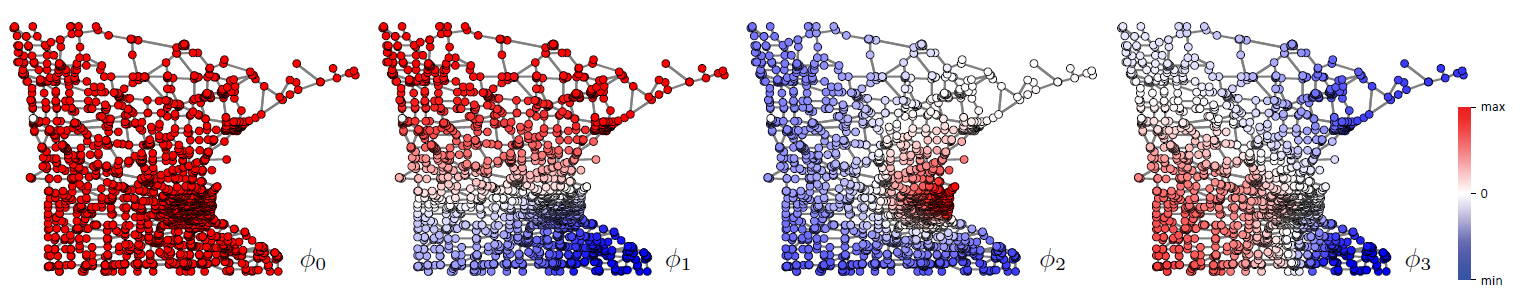
\includegraphics[width = \textwidth]{Images/Minnesota.png}
    \caption{Laplacian eigenfunctions on the graph representing the roads in Minnesota (from paper \cite{Beyound_eucl_data})}
    \label{fig:Minnesota}
\end{figure}

In \Cref{fig:Minnesota} is shown the graph representing the roads in Minnesota (USA).
On the same graph are illustrated the trends of four different eigenfunctions of the Laplacian matrix.
The one on the left represents the eigenfunction $\phi_0$ with the lowest possible Dirichlet energy and, as we have seen, it is exactly the constant function.
The other figures show other eigenfunctions of $L$ with higher Dirichlet energy values, therefore are more ``spiky'' than $\phi_0$.

\section{Heat Diffusion Equation}
\label{sec:heat_equation}

We can employ what we have learnt in the previous sections to write the heat equation on graphs.
Recall that in general the heat equation is written as
\begin{equation}
\label{eq:heat_eq_classic}
\begin{cases}
    \partial_t T(x,t) = c \Delta T(x,t) \\
    T(x,0) = T_0 (x) 
\end{cases}
\end{equation}
where $T(x,t)$ is the temperature at point $x$ at time $t$ and $\Delta$ is the laplacian operator.
The second equation represents the initial condition.
$c$ is referred to as the \emph{thermal diffusivity constant}.

Before writing the heat equation on graphs, let us talk about others definition of the discrete Laplacian.
In \Cref{def:laplacian}, we defined it as 
\begin{equation*}
    L \coloneqq A - D .
\end{equation*}
In the paper \cite{Beyound_eucl_data}, M. Bronstein defines $L$ as
\begin{equation*}
    L = M^{-1} (A-D) ,
\end{equation*}
where $M$ is a given matrix.
Clearly, if we choose $M = I$, we get the same Laplacian matrix we defined in \Cref{def:laplacian}.
If, however, we put $M = D$, where $D$ is the degree matrix, we obtain what is known as \emph{diffusive Laplacian}.
\begin{definition}
\label{def:diffusive_laplacian}
Let $\mathcal{G}(\mathcal{V}, \mathcal{E})$ be a graph, $A$ its adjacency matrix and $D$ its degree matrix.
The \emph{diffusive Laplacian} of the graph is
\begin{equation*}
    L = D^{-1} (A - D) = D^{-1} A - I .
\end{equation*}
\end{definition}

We are interested in the heat diffusion equation on a graph.
If we assume the thermal diffusivity constant $c$ to be equal to $1$ for the sake of simplicity, we can write the discrete version of \Cref{eq:heat_eq_classic} as
\begin{equation}
\label{eq:heat_eq_L}
    \partial _t h(v, t) = L h(v, t) ,
\end{equation}
where $h$ represents the temperature on the graph (or in general a signal) and is a function in $\mathbb{R}^{\mathcal{V}}$, depending on the time $t$.
We can solve this equation writing $h$ as a linear combination of the eigenfunctions $\phi _i$ of the Laplacian $L$:
\begin{equation*}
    h (t) = \sum_{i=1} ^ n a_i (t) \phi _i ,
\end{equation*}
where $a_i(t)= \langle h(t), \phi _i \rangle$.
Substituting this into \Cref{eq:heat_eq_L} gives us:
\begin{align*}
    &\sum _{i=1} ^n (\partial _t a_i(t) ) \phi _i(v) = 
    \sum _{i=1} ^n a_i(t) L \phi _i(v) =
    \sum _{i=1} ^n a_i(t) \lambda_i \phi _i(v) \\
    &\sum _{i=1} ^n \left( \partial _t a_i(t) - \lambda _i a_i(t) \right) \phi _i (v) =0 .
\end{align*}
Since the eigenfunctions $\phi _i$ are orthogonal to each other, we are left with $n$ differential equations for the coefficients $a_i(t)$:
\begin{equation*}
    \partial _t a_i(t) - \lambda _i a_i(t) = 0 .
\end{equation*}
These can be easily solved with exponential solutions:
\begin{equation*}
    a_i(t) = a_i (0) \exp (\lambda _i t) = a_i (0) \exp (- |\lambda _i| t) \Longrightarrow h(t) = \sum_{i=1} ^n a_i(0) \exp (- |\lambda _i| t) \phi _i .
\end{equation*}
Notice that as $t$ goes to infinity, the solution tends to the uniform eigenfunction $\phi _1$, how we would expect:
\begin{equation*}
    \lim_{t \to \infty} h(t) = \lim_{t \to \infty} \sum_{i=1} ^n a_i(0) \exp (- |\lambda _i| t) \phi _i =
    a_1(0) \phi_1 .
\end{equation*}

\begin{figure}[b]
    \centering
    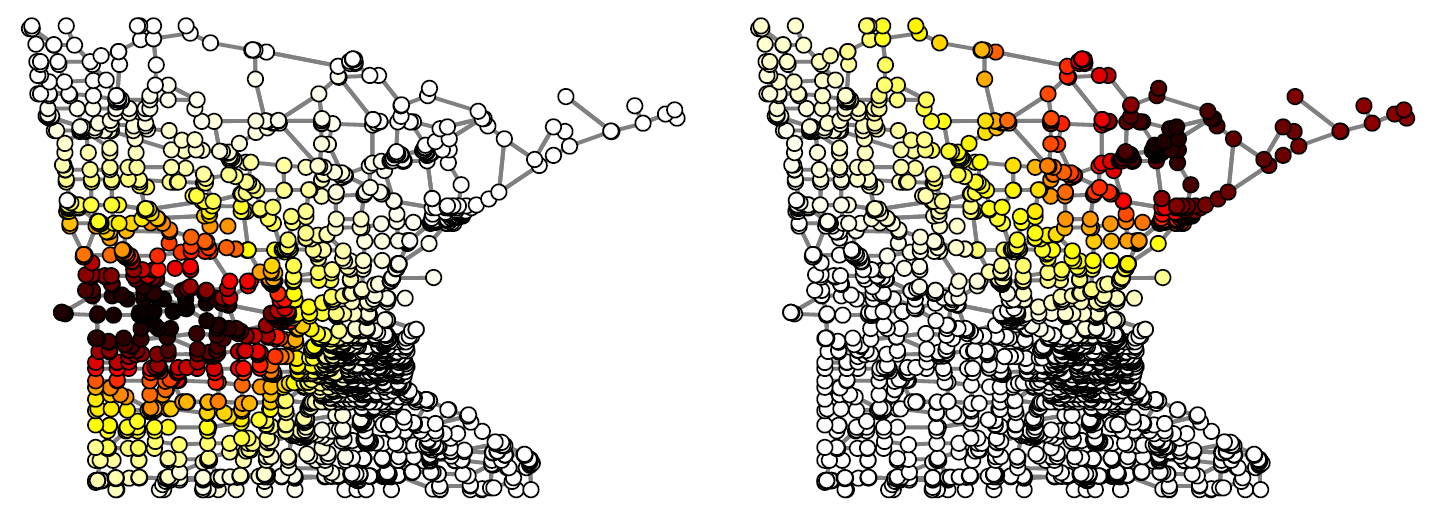
\includegraphics[width = 0.8 \textwidth]{Images/heat_diffusion.png}
    \caption{Example of heat diffusion on a graph (from paper \cite{Beyound_eucl_data})}
    \label{fig:heat_diffusion}
\end{figure}

We now look briefly at the heat diffusion equation with the diffusive Laplacian, since it will be useful later on.
If we still assume to have the thermal diffusivity constant $c$ equal to $1$, then \Cref{eq:heat_eq_L} can be written as
\begin{equation*}
    \partial _t h(v, t) = ( D^{-1} A - I ) h(v, t) .
\end{equation*}
If we also assume the time to be discrete, then the time derivative of $h(t)$ is simply $h_{t+1}- h_t$:
\begin{equation*}
    h_{t+1}(v) - h_t(v) = D^{-1} A h_t(v) - h_t(v) \Longrightarrow h_{t+1}(v) = D^{-1} A h_t(v) .
\end{equation*}
We already saw that
\begin{equation*}
    D^{-1} A h_t (v) = \sum_{u \in \mathcal{N}(v)} \frac{h_t(u)}{\deg (v)} .
\end{equation*}
Thus, the value of function $h$ at time $t+1$ at node $v$ depends on the sum of the values of the same function $h$ at time $t$ on the neighbours of node $v$, normalized with the degree $\deg (v)$.
This should remind us of a diffusive process on the graph.
If we iterate this over and over we will have a linear recursion
\begin{equation*}
    h_{t+1} (v) = \sum_{u \in \mathcal{N}(v)} \frac{h_t(u)}{\deg (v)}
\end{equation*}
where its fixed point is, again, the first eigenfunction $\phi _1$.

In \Cref{fig:heat_diffusion} are illustrated two examples of heat diffusion on a graph representing the roads in Minnesota.
Observe how moving the heat source to a different location changes the shape of the diffusion, which is an indication of the lack of shift-invariance on graphs.


%We now use this new definition of diffusive laplacian to find the discrete analogous of \Cref{eq:heat_eq_classic}. If we assume $c$ to be equal to one for the %sake of simplicity, we get
%\begin{equation*}
%    \partial _t h(v, t) = ( D^{-1} A - I ) h(v, t) .
%\end{equation*}
%$h$ represents the signal on the graph and is therefore a function in $\mathbb{R}^{\mathcal{V}}$ depending on the time $t$.
%If we also assume the time to be discrete, then the time derivative of $h(t)$ is simply $h_{t+1}- h_t$:
%\begin{equation*}
%    h_{t+1}(v) - h_t(v) = D^{-1} A h_t(v) - h_t(v) \Longrightarrow h_{t+1}(v) = D^{-1} A h_t(v) = \frac{A h_t(v)}{\deg (v)}.
%\end{equation*}
%We can easily find the solutions of 



\chapter{Geometric Deep Learning}
\label{cap:GDL}

In this chapter we discuss some methods and algorithms used to analyse geometric data based on the notions developed in the previous chapters.
When working with graphs, we can classify the main tasks roughly as follows:
\begin{itemize}
    \item \textbf{node classification}: we are given a graph and the features of only a small fraction of the nodes, and we want to predict the features of the remaining nodes;
    \item \textbf{edge classification}: similarly, we are given a graph and the features associated with some of the edges and we want to predict the features of the remaining edges;
    \item \textbf{graph classification}: we are given a number of different graphs, each labelled, and we want to learn to predict the labels of other graphs.
\end{itemize}
There are other classification tasks, however we shall not treat them in this thesis.
For more details see \cite{Beyound_eucl_data}, \cite{Kipf_welling}.

We shall concentrate in this chapter on the the first of these tasks: the node classification.
We will see some of the methods employed to classify the nodes of a graph, like graphSAGE neural networks and GATs.
Then we will apply one of these methods on the Zachary Karate Club (\cite{Kipf_welling}) dataset to elucidate practically the results.

\section{Encoder and Decoder}
\label{sec:encoder}

We start by discussing the \emph{encoder-decoder framework}, which is the base for building \emph{Geometric Convolutional Networks} (GCNs), the first kind of network we consider for node classification task.

We recall that in deep learning we classify images or more general data coming in a grid, that we call Euclidean data.
A deep learning network or CNN training works according to the following steps:
\begin{itemize}
    \item a series of convolutions and linear layers to compute a score associated to a datum;
    \item a loss function to compute the error in the prediction of the correct class of the given datum, obtained via forward pass;
    \item an update of the parameters through backpropagation via stochastic gradient descent pass.
\end{itemize}

In the case of non-euclidean data like graphs, the general structure of the learning process is the same.
%\begin{equation*}
%    \text{forward pass}\rightarrow \text{loss function}\rightarrow \text{backpropagation} ,
%\end{equation*}
The forward pass process, however, occurs differently and has to be adapted to the data.
In fact, there are some issues that have to be considered when dealing with data distributed according to a graph, like the geometric structure of the graph itself that needs to be given to the neural network.
To do so, we use the encoder-decoder framework.

We now assume to have a node classification task, this means that we are given a graph $\mathcal{G}(\mathcal{V}, \mathcal{E})$ and a vector of $m$ features for each node $v$, that we shall denote with $\mathbf{x}_v$ in $\mathbb{R}^m$.
We can therefore represent the data as a matrix
\begin{equation*}
    X = ( \mathbf{x}_1, \mathbf{x}_2, \ldots ,\mathbf{x}_n) \in \mathbb{R}^{m \times n}
\end{equation*}
where $n$ is the number of nodes in the graph $\mathcal{G}$.

Our goal is to make the network learn a \emph{node embedding} for every node of the graph, that is a function which associates a $p$-dimensional vector to each node $v$.
If we denote such embedding as $f$, we can write it as
\begin{align*}
    f : \mathcal{V} &\longrightarrow \mathbb{R}^p \\
    v &\longrightarrow \mathbf{z}_v .
\end{align*}
Generally, the dimension of $\mathbb{R}^p$ is chosen to be much smaller than the space of the features $\mathbb{R}^n$.
This function $f$ which provides the embedding of every node is called a \emph{node encoder}.
Even though we have defined the encoder for node classification task, it is possible to generalise this concept also for edge and graph classification tasks, but we do not treat those here.

%It is important to say that the encoder $f$ must `know' the topological structure of the graph considered.
%In fact, its role is to encapsulate that information somehow inside the node embeddings, in order to make it easier to complete the task.

The node embedding $f(\textbf{x}_v)$ provided by the encoder is then given to a \emph{decoder}, typically a simple linear classifier.
The output values are similar to the scores for each class for a SVM loss or to their probabilities for the cross-entropy loss we discussed in \Cref{sec:loss}.
The output takes values in $\mathbb{R}^c$, where $c$ is the number of classes.

The process of encoding and decoding described above is called \emph{forward pass}.
It is very similar to the forward pass of an ANN.
In fact, the main difference is how the encoder is implemented, since it has to take into account also the geometric information, which is fundamental when working with non-Euclidean data.

Once the decoder has provided an output, it is used to compute the loss function as we have seen for deep learning, and then the parameters characterizing the encoder and the decoder are updated through backpropagation. 

\section{GraphSAGE}
\label{sec:graphsage}

We now discuss a simple method to implement the encoder of an encoder-decoder framework.
We do not focus on the implementation of the decoder since it is much more straightforward and similar to the architectures seen in \Cref{cap:NN}.
The encoder, instead, has to find a way to deal with the complex topological structure of graphs.
The following algorithms are taken from the paper \cite{graphsage}.

Assume we have a graph $\mathcal{G}(\mathcal{V}, \mathcal{E})$, and to each node $v$ is associated a feature $\mathbf{h}_v$.
We want to find a general algorithm that gives us the node embeddings.
In order to find these embeddings, we have to consider the topology of our graph.
An iteration of a GraphSAGE convolution can be described schematically as:
\begin{enumerate}
    \item ${^k \mathbf{h}_{\mathcal{N}(v)}} = \text{AGGREGATE}(\{ {^{k-1}\mathbf{h}_u} , \forall u \in \mathcal{N}(v) \} )$;
    \item $ ^k \mathbf{h}_v ' = \text{CONCAT}({^k \mathbf{h}_{\mathcal{N}(v)}},  { ^{k-1} \mathbf{h}_v)}$;
    \item $^k \mathbf{h}_v '' = \sigma (W^k \cdot {^k\mathbf{h}_v '}) $;
    \item $^k \mathbf{h}_v  = {^k \mathbf{h}_v ''}/||{^k \mathbf{h}_v ''}||_2$.
\end{enumerate}
where we use the notation:
\begin{itemize}
    \item $k$ stands for the $k$-th iteration of the convolution;
    \item AGGREGATE is a generic aggregator function;
    \item CONCAT is a function which concatenates ${^k \mathbf{h}_{\mathcal{N}(v)}}$ and ${ ^{k-1} \mathbf{h}_v}$;
    \item $W^k$ is the weight matrix associated with the $k$-th layer of the convolution;
    \item $\sigma$ is the activation function.
\end{itemize}

To complete the convolution, we have to repeat the same process for every node $v \in \mathcal{V}$ and iterate this process for every convolutional layer of our neural network.
Notice how the change of dimensionality happens in passage $3$ when multiplying ${^k\mathbf{h}_v '}$ with $W^k$, in fact the size of the matrix $W^k$ decides the new dimension of the vector $^k \mathbf{h}_v $.
The final representations output after $K$ iterations is the node embedding $\mathbf{z}_v = { ^K \mathbf{h}_v}, \forall v \in \mathcal{V}$.

Until now we have left the definition of the aggregator function free of conditions, but notice how ideally it should be invariant to permutations of its inputs.
In fact, unlike the machine learning over images, the vertices of a graph have no natural ordering, thus the aggregator function must operate over an unordered set of vertices.

Furthermore notice how, since there is no way to use a filter scrolling through the data as in convolutional neural networks, the features of a node are passed to its neighbours.
This process is often referred to as \emph{message passing}.

\begin{figure}
    \centering
\begin{tikzpicture}[x=0.75pt,y=0.75pt,yscale=-1,xscale=1]
%uncomment if require: \path (0,300); %set diagram left start at 0, and has height of 300

%Shape: Ellipse [id:dp49210735500886793] 
\draw  [color={rgb, 255:red, 208; green, 2; blue, 27 }  ,draw opacity=1 ][fill={rgb, 255:red, 208; green, 2; blue, 27 }  ,fill opacity=1 ] (263.09,168.62) .. controls (263.09,165.33) and (265.72,162.67) .. (268.96,162.67) .. controls (272.21,162.67) and (274.84,165.33) .. (274.84,168.62) .. controls (274.84,171.91) and (272.21,174.58) .. (268.96,174.58) .. controls (265.72,174.58) and (263.09,171.91) .. (263.09,168.62) -- cycle ;
%Shape: Ellipse [id:dp29138004235720727] 
\draw  [draw opacity=0][fill={rgb, 255:red, 39; green, 132; blue, 242 }  ,fill opacity=1 ] (298.35,156.71) .. controls (298.35,153.42) and (300.98,150.75) .. (304.23,150.75) .. controls (307.47,150.75) and (310.11,153.42) .. (310.11,156.71) .. controls (310.11,160) and (307.47,162.67) .. (304.23,162.67) .. controls (300.98,162.67) and (298.35,160) .. (298.35,156.71) -- cycle ;
%Straight Lines [id:da010224704017222752] 
\draw    (274.47,165.49) -- (298.65,158.68) ;
%Straight Lines [id:da561176889911901] 
\draw    (237.56,148.37) -- (263.39,165.49) ;
%Straight Lines [id:da8144300982761781] 
\draw    (273.9,172.54) -- (311.42,211.44) ;
%Straight Lines [id:da15448762749533573] 
\draw    (268.96,162.67) -- (278.84,138.6) ;
%Straight Lines [id:da9214932123581858] 
\draw    (262.72,170.53) -- (239.21,177.68) ;
%Shape: Ellipse [id:dp3360392858084409] 
\draw   (263.76,227.84) .. controls (263.76,224.55) and (266.39,221.89) .. (269.64,221.89) .. controls (272.88,221.89) and (275.51,224.55) .. (275.51,227.84) .. controls (275.51,231.13) and (272.88,233.8) .. (269.64,233.8) .. controls (266.39,233.8) and (263.76,231.13) .. (263.76,227.84) -- cycle ;
%Shape: Ellipse [id:dp7890364244796149] 
\draw  [draw opacity=0][fill={rgb, 255:red, 65; green, 117; blue, 5 }  ,fill opacity=0.86 ] (310.11,132.89) .. controls (310.11,129.6) and (312.74,126.93) .. (315.98,126.93) .. controls (319.23,126.93) and (321.86,129.6) .. (321.86,132.89) .. controls (321.86,136.18) and (319.23,138.84) .. (315.98,138.84) .. controls (312.74,138.84) and (310.11,136.18) .. (310.11,132.89) -- cycle ;
%Straight Lines [id:da8493851937056023] 
\draw [color={rgb, 255:red, 21; green, 120; blue, 236 }  ,draw opacity=0.73 ][fill={rgb, 255:red, 65; green, 117; blue, 5 }  ,fill opacity=1 ][line width=2.25]    (278.84,138.6) -- (270.86,158.04) ;
\draw [shift={(268.96,162.67)}, rotate = 292.31] [fill={rgb, 255:red, 21; green, 120; blue, 236 }  ,fill opacity=0.73 ][line width=0.08]  [draw opacity=0] (8.57,-4.12) -- (0,0) -- (8.57,4.12) -- cycle    ;
%Straight Lines [id:da05541020182657119] 
\draw [color={rgb, 255:red, 21; green, 120; blue, 236 }  ,draw opacity=0.73 ][fill={rgb, 255:red, 65; green, 117; blue, 5 }  ,fill opacity=1 ][line width=2.25]    (298.65,158.68) -- (279.29,164.14) ;
\draw [shift={(274.47,165.49)}, rotate = 344.28] [fill={rgb, 255:red, 21; green, 120; blue, 236 }  ,fill opacity=0.73 ][line width=0.08]  [draw opacity=0] (8.57,-4.12) -- (0,0) -- (8.57,4.12) -- cycle    ;
%Straight Lines [id:da24832309977919587] 
\draw [color={rgb, 255:red, 21; green, 120; blue, 236 }  ,draw opacity=0.73 ][fill={rgb, 255:red, 65; green, 117; blue, 5 }  ,fill opacity=1 ][line width=2.25]    (311.42,211.44) -- (277.37,176.14) ;
\draw [shift={(273.9,172.54)}, rotate = 46.04] [fill={rgb, 255:red, 21; green, 120; blue, 236 }  ,fill opacity=0.73 ][line width=0.08]  [draw opacity=0] (8.57,-4.12) -- (0,0) -- (8.57,4.12) -- cycle    ;
%Straight Lines [id:da3007928238057245] 
\draw [color={rgb, 255:red, 21; green, 120; blue, 236 }  ,draw opacity=0.73 ][fill={rgb, 255:red, 65; green, 117; blue, 5 }  ,fill opacity=1 ][line width=2.25]    (239.21,177.68) -- (257.93,171.98) ;
\draw [shift={(262.72,170.53)}, rotate = 163.09] [fill={rgb, 255:red, 21; green, 120; blue, 236 }  ,fill opacity=0.73 ][line width=0.08]  [draw opacity=0] (8.57,-4.12) -- (0,0) -- (8.57,4.12) -- cycle    ;
%Straight Lines [id:da9480906622955794] 
\draw [color={rgb, 255:red, 21; green, 120; blue, 236 }  ,draw opacity=0.73 ][fill={rgb, 255:red, 65; green, 117; blue, 5 }  ,fill opacity=1 ][line width=2.25]    (237.56,148.37) -- (259.22,162.73) ;
\draw [shift={(263.39,165.49)}, rotate = 213.54] [fill={rgb, 255:red, 21; green, 120; blue, 236 }  ,fill opacity=0.73 ][line width=0.08]  [draw opacity=0] (8.57,-4.12) -- (0,0) -- (8.57,4.12) -- cycle    ;
%Straight Lines [id:da9838247948059811] 
\draw    (317.63,138.2) -- (327.74,174.58) ;
%Straight Lines [id:da9794815756254049] 
\draw    (307.89,160.32) -- (323.17,176.31) ;
%Straight Lines [id:da39966345372793866] 
\draw    (285.39,207.29) -- (310.11,216.27) ;
%Straight Lines [id:da34014965132362085] 
\draw    (238.2,220.22) -- (263.76,227.84) ;
%Straight Lines [id:da8157466821673056] 
\draw    (233.7,186.49) -- (233.7,210.32) ;
%Straight Lines [id:da11748963504972587] 
\draw    (214.86,171.55) -- (227.79,178.19) ;
%Straight Lines [id:da5566362409919412] 
\draw    (313.77,138.2) -- (307.38,151.81) ;
%Straight Lines [id:da5827613012121686] 
\draw    (290.09,102.8) -- (283.54,126.96) ;
%Straight Lines [id:da6766490461751147] 
\draw    (252.64,124.92) -- (237.53,139.9) ;
%Straight Lines [id:da6558519763690789] 
\draw [color={rgb, 255:red, 65; green, 117; blue, 5 }  ,draw opacity=0.77 ][fill={rgb, 255:red, 65; green, 117; blue, 5 }  ,fill opacity=1 ][line width=2.25]    (323.17,176.31) -- (311.34,163.93) ;
\draw [shift={(307.89,160.32)}, rotate = 46.31] [fill={rgb, 255:red, 65; green, 117; blue, 5 }  ,fill opacity=0.77 ][line width=0.08]  [draw opacity=0] (8.57,-4.12) -- (0,0) -- (8.57,4.12) -- cycle    ;
%Straight Lines [id:da5381258226258809] 
\draw [color={rgb, 255:red, 65; green, 117; blue, 5 }  ,draw opacity=0.77 ][fill={rgb, 255:red, 65; green, 117; blue, 5 }  ,fill opacity=1 ][line width=2.25]    (313.77,138.2) -- (309.51,147.28) ;
\draw [shift={(307.38,151.81)}, rotate = 295.11] [fill={rgb, 255:red, 65; green, 117; blue, 5 }  ,fill opacity=0.77 ][line width=0.08]  [draw opacity=0] (8.57,-4.12) -- (0,0) -- (8.57,4.12) -- cycle    ;
%Straight Lines [id:da42368478456642134] 
\draw [color={rgb, 255:red, 65; green, 117; blue, 5 }  ,draw opacity=0.77 ][fill={rgb, 255:red, 65; green, 117; blue, 5 }  ,fill opacity=1 ][line width=2.25]    (285.39,207.29) -- (305.41,214.56) ;
\draw [shift={(310.11,216.27)}, rotate = 199.98] [fill={rgb, 255:red, 65; green, 117; blue, 5 }  ,fill opacity=0.77 ][line width=0.08]  [draw opacity=0] (8.57,-4.12) -- (0,0) -- (8.57,4.12) -- cycle    ;
%Straight Lines [id:da6333741564176212] 
\draw [color={rgb, 255:red, 65; green, 117; blue, 5 }  ,draw opacity=0.77 ][fill={rgb, 255:red, 65; green, 117; blue, 5 }  ,fill opacity=1 ][line width=2.25]    (233.7,210.32) -- (233.7,191.49) ;
\draw [shift={(233.7,186.49)}, rotate = 90] [fill={rgb, 255:red, 65; green, 117; blue, 5 }  ,fill opacity=0.77 ][line width=0.08]  [draw opacity=0] (8.57,-4.12) -- (0,0) -- (8.57,4.12) -- cycle    ;
%Straight Lines [id:da9488859654017616] 
\draw [color={rgb, 255:red, 65; green, 117; blue, 5 }  ,draw opacity=0.77 ][fill={rgb, 255:red, 65; green, 117; blue, 5 }  ,fill opacity=1 ][line width=2.25]    (214.86,171.55) -- (223.34,175.9) ;
\draw [shift={(227.79,178.19)}, rotate = 207.17] [fill={rgb, 255:red, 65; green, 117; blue, 5 }  ,fill opacity=0.77 ][line width=0.08]  [draw opacity=0] (8.57,-4.12) -- (0,0) -- (8.57,4.12) -- cycle    ;
%Straight Lines [id:da9817458545679609] 
\draw [color={rgb, 255:red, 65; green, 117; blue, 5 }  ,draw opacity=0.77 ][fill={rgb, 255:red, 65; green, 117; blue, 5 }  ,fill opacity=1 ][line width=2.25]    (252.64,124.92) -- (241.08,136.38) ;
\draw [shift={(237.53,139.9)}, rotate = 315.26] [fill={rgb, 255:red, 65; green, 117; blue, 5 }  ,fill opacity=0.77 ][line width=0.08]  [draw opacity=0] (8.57,-4.12) -- (0,0) -- (8.57,4.12) -- cycle    ;
%Straight Lines [id:da1928414104273437] 
\draw [color={rgb, 255:red, 65; green, 117; blue, 5 }  ,draw opacity=0.77 ][fill={rgb, 255:red, 65; green, 117; blue, 5 }  ,fill opacity=1 ][line width=2.25]    (290.09,102.8) -- (284.85,122.14) ;
\draw [shift={(283.54,126.96)}, rotate = 285.16] [fill={rgb, 255:red, 65; green, 117; blue, 5 }  ,fill opacity=0.77 ][line width=0.08]  [draw opacity=0] (8.57,-4.12) -- (0,0) -- (8.57,4.12) -- cycle    ;
%Shape: Ellipse [id:dp7783662551333383] 
\draw  [draw opacity=0][fill={rgb, 255:red, 39; green, 132; blue, 242 }  ,fill opacity=1 ] (274.84,132.89) .. controls (274.84,129.6) and (277.47,126.93) .. (280.72,126.93) .. controls (283.97,126.93) and (286.6,129.6) .. (286.6,132.89) .. controls (286.6,136.18) and (283.97,138.84) .. (280.72,138.84) .. controls (277.47,138.84) and (274.84,136.18) .. (274.84,132.89) -- cycle ;
%Shape: Ellipse [id:dp8965905411482669] 
\draw  [draw opacity=0][fill={rgb, 255:red, 39; green, 132; blue, 242 }  ,fill opacity=1 ] (310.11,216.27) .. controls (310.11,212.98) and (312.74,210.32) .. (315.98,210.32) .. controls (319.23,210.32) and (321.86,212.98) .. (321.86,216.27) .. controls (321.86,219.56) and (319.23,222.23) .. (315.98,222.23) .. controls (312.74,222.23) and (310.11,219.56) .. (310.11,216.27) -- cycle ;
%Shape: Ellipse [id:dp5045155209768624] 
\draw  [draw opacity=0][fill={rgb, 255:red, 39; green, 132; blue, 242 }  ,fill opacity=1 ] (227.82,180.53) .. controls (227.82,177.25) and (230.46,174.58) .. (233.7,174.58) .. controls (236.95,174.58) and (239.58,177.25) .. (239.58,180.53) .. controls (239.58,183.82) and (236.95,186.49) .. (233.7,186.49) .. controls (230.46,186.49) and (227.82,183.82) .. (227.82,180.53) -- cycle ;
%Shape: Ellipse [id:dp9587679586971831] 
\draw  [draw opacity=0][fill={rgb, 255:red, 39; green, 132; blue, 242 }  ,fill opacity=1 ] (227.82,144.8) .. controls (227.82,141.51) and (230.46,138.84) .. (233.7,138.84) .. controls (236.95,138.84) and (239.58,141.51) .. (239.58,144.8) .. controls (239.58,148.09) and (236.95,150.75) .. (233.7,150.75) .. controls (230.46,150.75) and (227.82,148.09) .. (227.82,144.8) -- cycle ;
%Shape: Ellipse [id:dp10902948340206753] 
\draw  [draw opacity=0][fill={rgb, 255:red, 65; green, 117; blue, 5 }  ,fill opacity=0.86 ] (321.86,180.53) .. controls (321.86,177.25) and (324.49,174.58) .. (327.74,174.58) .. controls (330.98,174.58) and (333.61,177.25) .. (333.61,180.53) .. controls (333.61,183.82) and (330.98,186.49) .. (327.74,186.49) .. controls (324.49,186.49) and (321.86,183.82) .. (321.86,180.53) -- cycle ;
%Shape: Ellipse [id:dp7794729034258479] 
\draw  [draw opacity=0][fill={rgb, 255:red, 65; green, 117; blue, 5 }  ,fill opacity=0.86 ] (274.84,204.36) .. controls (274.84,201.07) and (277.47,198.4) .. (280.72,198.4) .. controls (283.97,198.4) and (286.6,201.07) .. (286.6,204.36) .. controls (286.6,207.65) and (283.97,210.32) .. (280.72,210.32) .. controls (277.47,210.32) and (274.84,207.65) .. (274.84,204.36) -- cycle ;
%Shape: Ellipse [id:dp9537764640039552] 
\draw  [draw opacity=0][fill={rgb, 255:red, 65; green, 117; blue, 5 }  ,fill opacity=0.86 ] (227.82,216.27) .. controls (227.82,212.98) and (230.46,210.32) .. (233.7,210.32) .. controls (236.95,210.32) and (239.58,212.98) .. (239.58,216.27) .. controls (239.58,219.56) and (236.95,222.23) .. (233.7,222.23) .. controls (230.46,222.23) and (227.82,219.56) .. (227.82,216.27) -- cycle ;
%Shape: Ellipse [id:dp14211007586651725] 
\draw  [draw opacity=0][fill={rgb, 255:red, 65; green, 117; blue, 5 }  ,fill opacity=0.86 ] (204.32,168.62) .. controls (204.32,165.33) and (206.95,162.67) .. (210.19,162.67) .. controls (213.44,162.67) and (216.07,165.33) .. (216.07,168.62) .. controls (216.07,171.91) and (213.44,174.58) .. (210.19,174.58) .. controls (206.95,174.58) and (204.32,171.91) .. (204.32,168.62) -- cycle ;
%Shape: Ellipse [id:dp12459730863844865] 
\draw  [draw opacity=0][fill={rgb, 255:red, 65; green, 117; blue, 5 }  ,fill opacity=0.86 ] (286.6,97.15) .. controls (286.6,93.86) and (289.23,91.19) .. (292.47,91.19) .. controls (295.72,91.19) and (298.35,93.86) .. (298.35,97.15) .. controls (298.35,100.44) and (295.72,103.1) .. (292.47,103.1) .. controls (289.23,103.1) and (286.6,100.44) .. (286.6,97.15) -- cycle ;
%Shape: Ellipse [id:dp8213766960689188] 
\draw  [draw opacity=0][fill={rgb, 255:red, 65; green, 117; blue, 5 }  ,fill opacity=0.86 ] (251.33,120.97) .. controls (251.33,117.68) and (253.96,115.02) .. (257.21,115.02) .. controls (260.46,115.02) and (263.09,117.68) .. (263.09,120.97) .. controls (263.09,124.26) and (260.46,126.93) .. (257.21,126.93) .. controls (253.96,126.93) and (251.33,124.26) .. (251.33,120.97) -- cycle ;
%Shape: Ellipse [id:dp2969931235099741] 
\draw   (204.32,144.8) .. controls (204.32,141.51) and (206.95,138.84) .. (210.19,138.84) .. controls (213.44,138.84) and (216.07,141.51) .. (216.07,144.8) .. controls (216.07,148.09) and (213.44,150.75) .. (210.19,150.75) .. controls (206.95,150.75) and (204.32,148.09) .. (204.32,144.8) -- cycle ;
%Straight Lines [id:da7231789562437343] 
\draw    (216.07,144.8) -- (227.82,144.8) ;
%Curve Lines [id:da7231646272123977] 
\draw [color={rgb, 255:red, 155; green, 155; blue, 155 }  ,draw opacity=1 ]   (322.49,100.54) .. controls (317.95,112.23) and (302.03,136.77) .. (279.44,146.68) ;
\draw [shift={(276.96,147.7)}, rotate = 339.09] [fill={rgb, 255:red, 155; green, 155; blue, 155 }  ,fill opacity=1 ][line width=0.08]  [draw opacity=0] (7.14,-3.43) -- (0,0) -- (7.14,3.43) -- cycle    ;
%Curve Lines [id:da05280946305613843] 
\draw [color={rgb, 255:red, 155; green, 155; blue, 155 }  ,draw opacity=1 ]   (262.49,83.4) .. controls (268.01,94.41) and (270.74,103.64) .. (283.74,109.99) ;
\draw [shift={(286.36,111.17)}, rotate = 202.58] [fill={rgb, 255:red, 155; green, 155; blue, 155 }  ,fill opacity=1 ][line width=0.08]  [draw opacity=0] (7.14,-3.43) -- (0,0) -- (7.14,3.43) -- cycle    ;

% Text Node
\draw  [color={rgb, 255:red, 155; green, 155; blue, 155 }  ,draw opacity=0.76 ]  (315.39,78.91) -- (412.39,78.91) -- (412.39,99.91) -- (315.39,99.91) -- cycle  ;
\draw (318.39,82.91) node [anchor=north west][inner sep=0.75pt]  [font=\scriptsize] [align=left] {AGGREGATOR$\displaystyle _{\text{1}}$};
% Text Node
\draw  [color={rgb, 255:red, 155; green, 155; blue, 155 }  ,draw opacity=0.76 ]  (189.61,62.63) -- (286.61,62.63) -- (286.61,83.63) -- (189.61,83.63) -- cycle  ;
\draw (192.61,66.63) node [anchor=north west][inner sep=0.75pt]  [font=\scriptsize] [align=left] {AGGREGATOR$\displaystyle _{\text{2}}$};


\end{tikzpicture}
    \caption{Aggregating feature information from neighbours with a two-step aggregator}
    \label{fig:message_passing}
\end{figure}

One among the possible way to implement this message passing is
\begin{equation}
\label{eq:convolution_aggregator}
    ^{k+1}\mathbf{h}_v = \sigma \left(W^k \sum _{u\in \mathcal{N}(v)} \frac{ ^k \mathbf{h}_u}{\deg (v)} + B^k \cdot {^k \mathbf{h}_v} \right) .
\end{equation}
The aggregator function is basically a mean of the vectors $\{ ^k \mathbf{h}_u, \forall u \in \mathcal{N}(v)\}$.
$W^K$ and $B^k$ are the weight matrices that have to be updated through backpropagation.
This aggregator is called \emph{convolutional} since it is a rough approximation of a localized spectral convolution.

If we focus only on the aggregator function of \Cref{eq:convolution_aggregator}, it is of the form
\begin{equation*}
    ^{k+1}\mathbf{h}_v = \sum _{u\in \mathcal{N}(v)} \frac{ ^k \mathbf{h}_u}{\deg (v)} = ( D^{-1} A ) {^{k}\mathbf{h}_v } ,
\end{equation*}
where $D$ is the degree matrix and $A$ the adjacency matrix.
\begin{equation*}
     ^{k+1}\mathbf{h}_v - {^{k}\mathbf{h}_v } =( D^{-1} A ) {^{k}\mathbf{h}_v } - {^{k}\mathbf{h}_v }  = (D^{-1}A - I) {^{k}\mathbf{h}_v } = D^{-1} (A - D) {^{k}\mathbf{h}_v } .
\end{equation*}
This is exactly the discrete heat diffusion equation we found in \Cref{sec:heat_equation}.
In fact, since the time is discrete, $^{k+1}\mathbf{h}_v - {^{k}\mathbf{h}_v }$ represents the time derivative of ${^{k}\mathbf{h}_v }$, while $D^{-1}(A-D)$ is the definition of diffusive Laplacian $L$:
\begin{equation*}
    \partial_t {^{k}\mathbf{h}_v } = L {^{k}\mathbf{h}_v }.
\end{equation*}
Thus the message passing defined in \Cref{eq:convolution_aggregator} spreads the information along the graph following the discretization of the equation describing how heat diffuses across an object.


\section{Graph Attention Networks}
\label{sec:GAT}

\emph{Graph Attention Networks} (GATs) are networks designed to ``pay attention'' to some links with respect to others.
The key idea is still to gather information during a convolutional iteration from the neighbouring nodes and put such information in a new vector.
This is what in \Cref{sec:graphsage} we called AGGREGATE and CONCAT functions.
Basically, we still want to find a way to aggregate the features, but this time we introduce the attention coefficients $\alpha _{vu}$ telling us the importance of the edge linking node $v$ to node $u$.

Let us now see how we can find the attention coefficients and use them to build a GAT for node classification.
We start by describing a single \emph{graph attentional layer}.
Let $W$ be a weight matrix and $\textbf{h}_v, \textbf{h}_u \in \mathbb{R}^d$ the features of nodes $v$ and $u$.
We define
\begin{alignat*}{3}
    a:  \mathbb{R}^{d'} &\times \mathbb{R}^{d'} &&\longrightarrow \mathbb{R} \\
          W \textbf{h}_v &\times W \textbf{h}_u &&\longrightarrow e_{vu} = a(W \textbf{h}_v, W \textbf{h}_u) .
\end{alignat*}
that indicates the importance associates to the link connecting $v$ to $u$.
Clearly, the more similar the features $W \textbf{h}_v$ and $W \textbf{h}_u$ are, the higher the importance associated is.

%Theoretically, this model allows to drop every geometric information since every node would be able to attend to every other node.
%We inject the graph structure by performing a \emph{mask attention}, that is computing the attention coefficient only on the neighbours of node $v$ (including $v$ itself).
%Notice, however, that in general the definition of neighbours could differ.
We then normalise $e_{vu}$ using the softmax function:
\begin{equation*}
    \alpha _{vu} = \text{SOFTMAX}_u (e_{vu}) = \frac{\exp (e_{vu})}{\sum _{w \in \mathcal{N}(v) \cup \{v\}} \exp (e_{vw})} .
\end{equation*}

Once the attention coefficients are computed, we can use them to gather the features from the neighbourhood of node $v$ into a new vector of features $\textbf{h}_v '$ through a linear combination, followed by an activation function $\sigma$:
\begin{equation*}
    \textbf{h}_v ' = \sigma \left( \sum_{u \in \mathcal{N}(v) \cup \{v\}} \alpha_{vu} W \textbf{h}_u \right) .
\end{equation*}

In the paper \cite{GATs}, Veličković \textit{et al.} choose an attention mechanism $a(W \textbf{h}_v, W \textbf{h}_u)$ as a single layer feedforward neural network characterised by a weight vector $\textbf{a} \in \mathbb{R}^{2 d'}$, applied to the concatenation of vectors $W \textbf{h}_v$ and $W \textbf{h}_u$, followed by a LeakyReLU non-linearity.
We can thus express the attention coefficients as
\begin{equation*}
    \alpha _{vu} = \frac{\exp \left( \sigma \left( \textbf{a}^{\top} [ W \textbf{h}_v || W \textbf{h}_u ] \right) \right)}
    {\sum _{w \in \mathcal{N}(v) \cup \{v\}} \exp \left( \sigma \left( \textbf{a}^{\top} [W \textbf{h}_v || W \textbf{}_w ] \right) \right)}
\end{equation*}
where $||$ is the concatenation operation and $\sigma$ is the LeakyReLU activation function.
A graphic representation of this mechanism is shown in \Cref{fig:GAT_article}.

\begin{figure}
\centering
\begin{subfigure}{.4\textwidth}
  \centering
  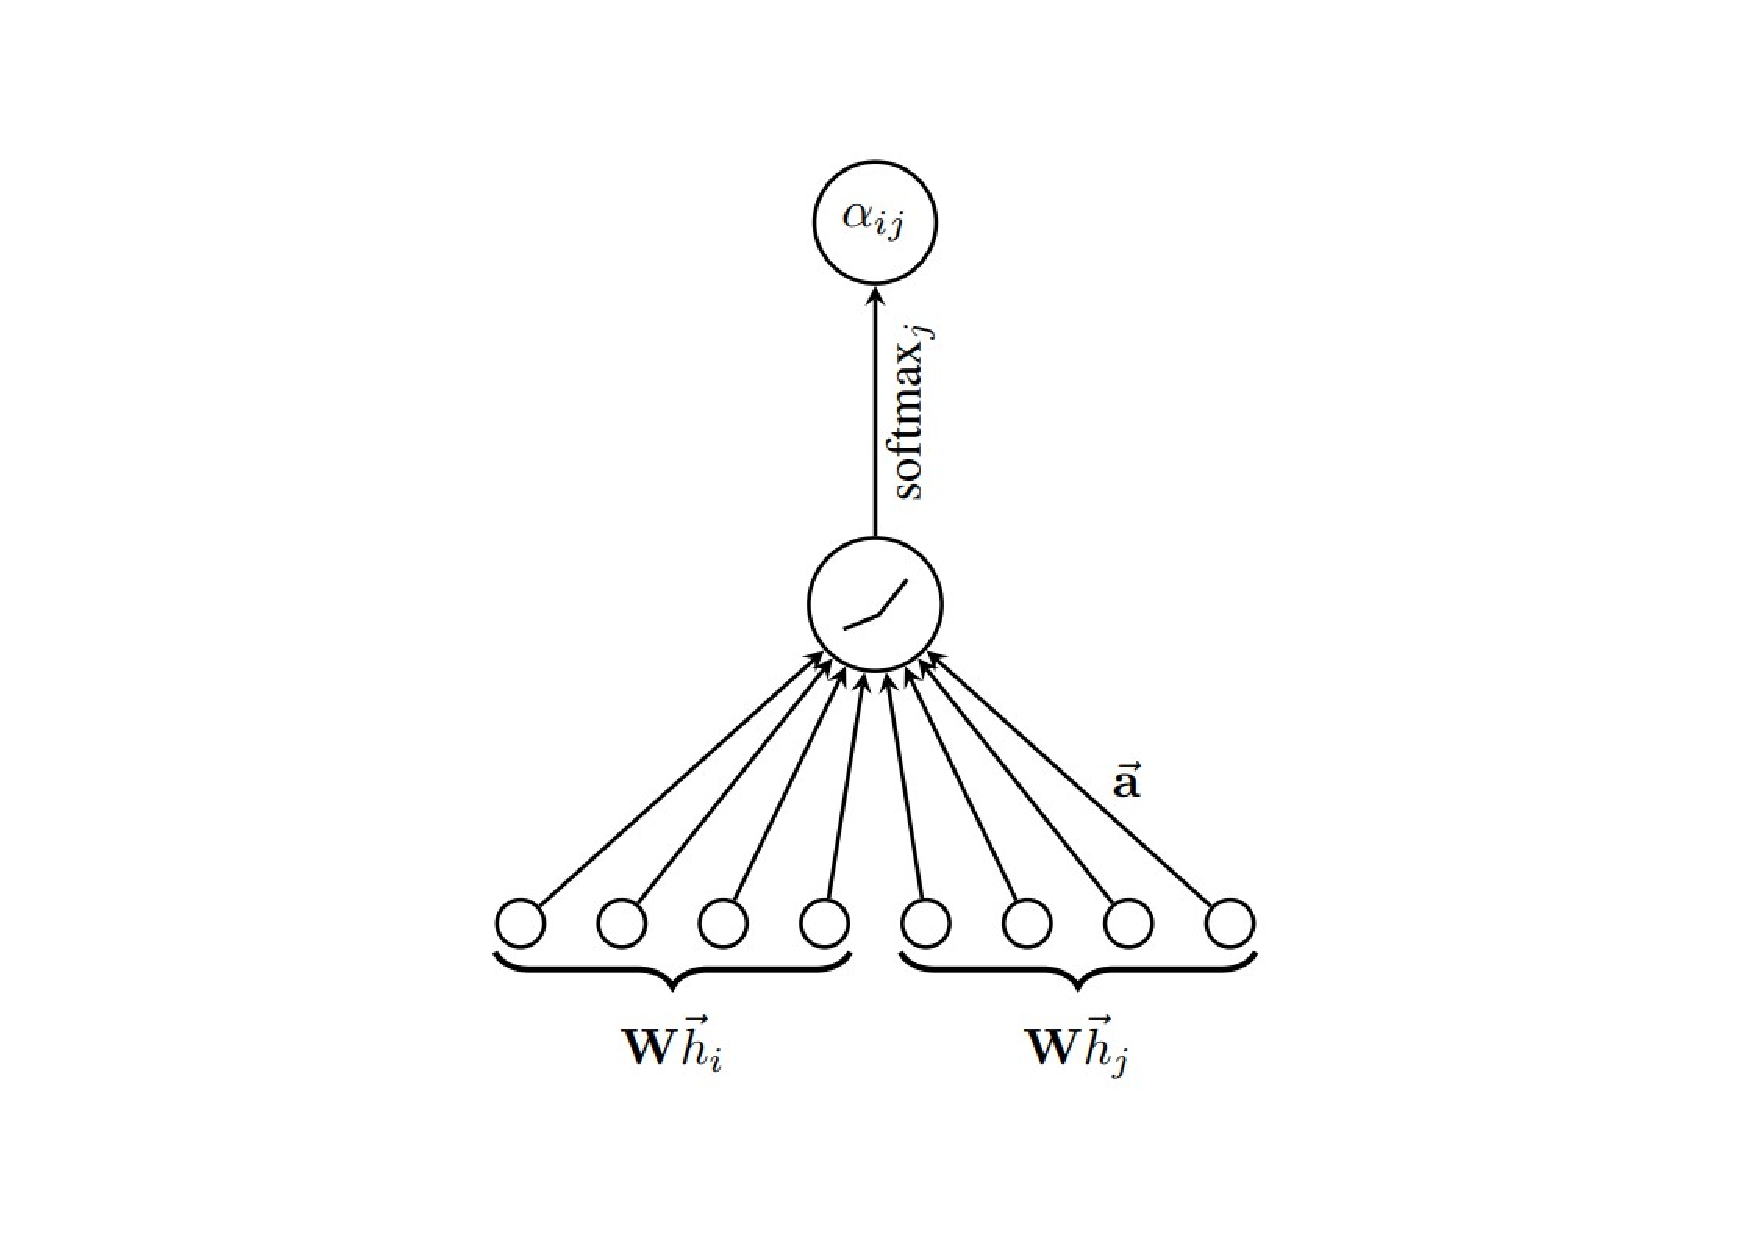
\includegraphics[trim={8cm 2.2cm 8cm 0}, clip,width=0.9\linewidth]{Images/GAT_article.pdf}
  \caption{Attention mechanism used by the authors}
  \label{fig:GAT_article}
\end{subfigure}
\begin{subfigure}{.58\textwidth}
  \centering
  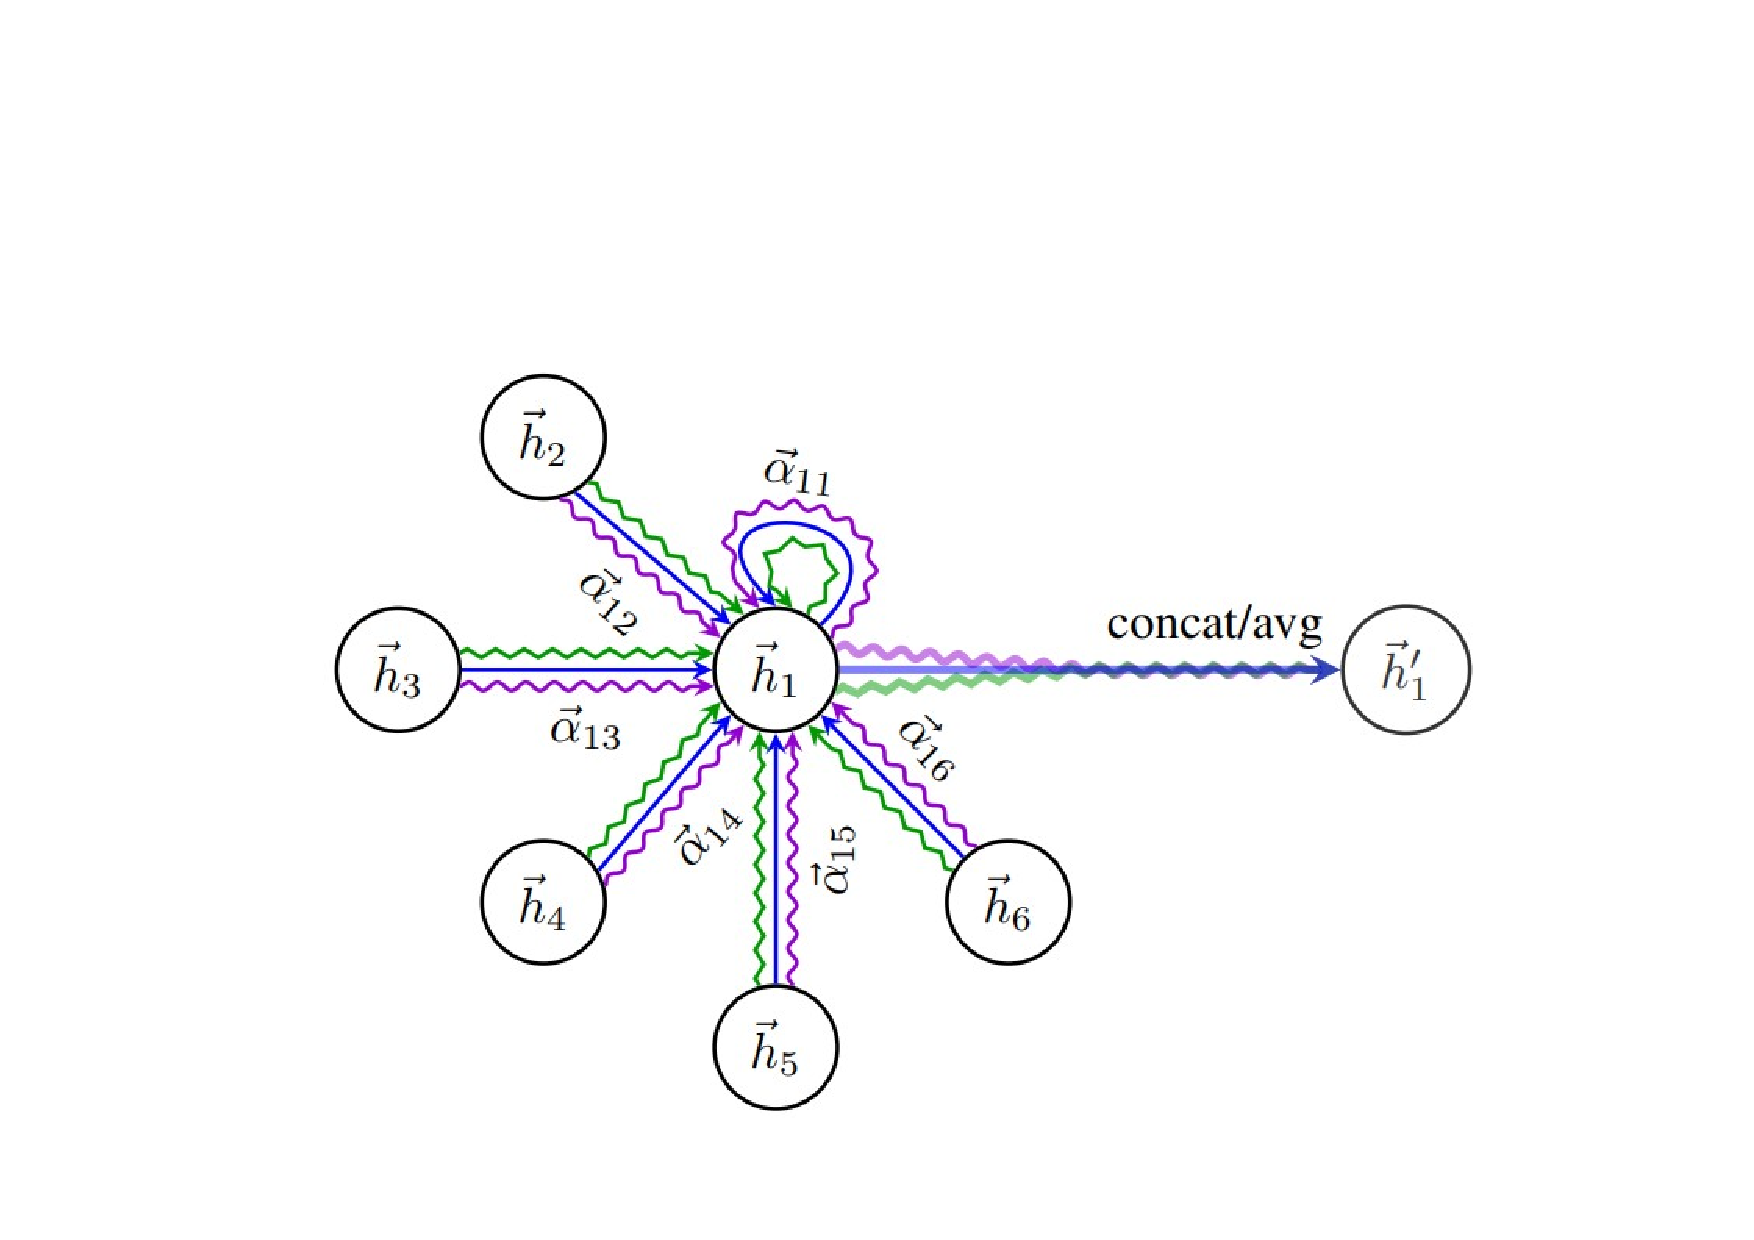
\includegraphics[trim={5cm 2.2cm 4.5cm 0}, clip,width=0.9\linewidth]{Images/GAT_multi_head.pdf}
  \caption{Illustration of multi-head attention with $K = 3$}
  \label{fig:GAT_multihead}
\end{subfigure}
\caption{Figures taken from paper \cite{GATs}}
\label{fig:GATs}
\end{figure}

Sometimes, to stabilize the learning process of self-attention, a \emph{multi-head attention} approach is employed.
$K$ independent parallel convolutions are applied to the same node $v$ (with different weight matrices $W^k$) and then their features are concatenated to get a final vector $\textbf{h}_v ' \in \mathbb{R}^{Kd'}$, that is
\begin{equation*}
    \textbf{h}_v ' = ||_{k=1} ^K \sigma \left( \sum_{u \in \mathcal{N}(v) \cup \{v\}} \alpha _{vu} ^k W^k \textbf{h}_v \right) .
\end{equation*}
where $\alpha _{vu}^k$ are the normalized attention coefficients computed by te $k$-th attention mechanism.
In \Cref{fig:GAT_multihead} is shown an example of multi-head attention; different arrow styles denote independent attention computations that are then concatenated together.

\section{Zachary Karate Club}
\label{sec:Zachary}

In this section we introduce the Zachary Karate Club dataset and then we use a graphSAGE convolutional neural network to classify the nodes.

The Zachary Karate Club is a social network of a karate club studied by W. Zachary in the article \cite{ZacharyKarateClub}.
The dataset consists in 34 members of the karate club, documenting 154 links between pairs of members who interacted outside the club.
After some time, from 1970 and 1972, the club became divided over an internal issue regarding the price of karate lessons.
Every node is thus labeled by one of four classes, obtained via modularity-based clustering (\cite{Modularity_clustering}).
See \Cref{fig:karateclub} for an illustration.

\begin{figure}
    \centering
    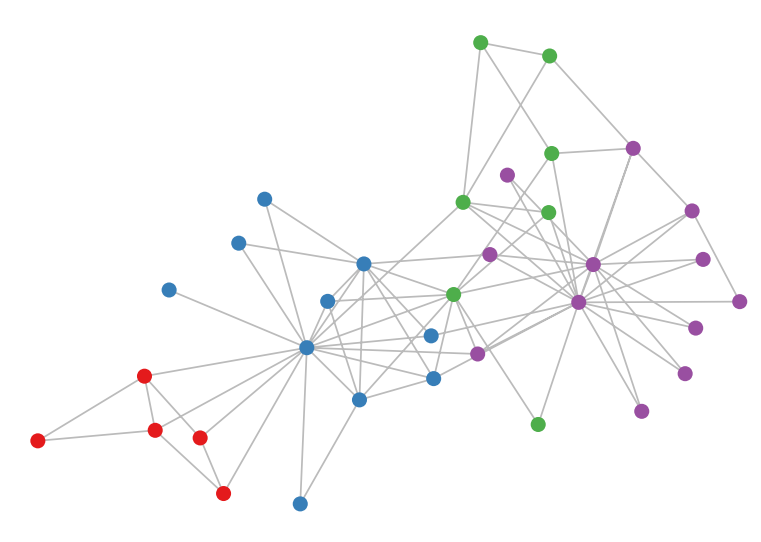
\includegraphics[width=0.55\textwidth]{Images/karate_club.png}
    \caption{Representation of the Zachary Karate Club dataset taken from paper \cite{Kipf_welling}}
    \label{fig:karateclub}
\end{figure}

We now use this dataset to build a graph neural network for the task of node classification.
We are given the labels for one node in each of the four groups.
Our goal is to classify the remaining 30 nodes between the 4 groups, considering their relations, i.e. the links between pairs of nodes.

We recall that a graphSAGE layer aggregator is implemented as
\begin{equation*}
    ^{k+1}\mathbf{h}_v = \sigma \left(W^k \sum _{u\in \mathcal{N}(v)} \frac{ ^k \mathbf{h}_u}{\deg (v)} + B^k \cdot {^k \mathbf{h}_v} \right) .
\end{equation*}
We take a featureless approach by setting the input matrix as
\begin{equation*}
    X = \left( \textbf{h}_1 ^0, \textbf{h}_2 ^0, \ldots, \textbf{h}_{34} ^0 \right) = I_{34} .
\end{equation*}
Note that the ordering of the nodes is random, therefore the ordering does not have meaning.
Our neural network takes the features in $\mathbb{R}^{34}$ and, by mean of a graphSAGE encoding convolution (SAGEconv), transforms it in a 4-dimensional vector.
The non-linearity $\sigma$ is chosen to be the $\tanh ()$ function.
In the second layer we keep the dimension of the first, while in the final passage we shrink the data into a 2-dimensional vector $\textbf{z}_v$ for every node $v$.
$\textbf{z}_v$ is the node embedding of $v$.
Thus, for each node, this algorithm gathers the information from 3-hops distance nodes and encodes them into the embeddings $\textbf{z}_v$.
Finally, we use a linear classifier to carry the embeddings in the output layer.
Since the possible labels are 4, the output vectors will be of size 4.
In \Cref{fig:encoder} is illustrated the encoder mechanism of our neural network.

\begin{figure}
    \centering
    \begin{tikzpicture}[x=0.75pt,y=0.75pt,yscale=-1,xscale=1]
    %uncomment if require: \path (0,300); %set diagram left start at 0, and has height of 300
    
    %Shape: Circle [id:dp8185238022426937] 
    \draw  [fill={rgb, 255:red, 126; green, 211; blue, 33 }  ,fill opacity=0.48 ] (140,70) .. controls (140,58.95) and (148.95,50) .. (160,50) .. controls (171.05,50) and (180,58.95) .. (180,70) .. controls (180,81.05) and (171.05,90) .. (160,90) .. controls (148.95,90) and (140,81.05) .. (140,70) -- cycle ;
    %Curve Lines [id:da9729407297561248] 
    \draw    (150,80) .. controls (165.33,80.5) and (157,60.5) .. (170,60) ;
    %Straight Lines [id:da4522339197676304] 
    \draw    (120,70) -- (137,70) ;
    \draw [shift={(140,70)}, rotate = 180] [fill={rgb, 255:red, 0; green, 0; blue, 0 }  ][line width=0.08]  [draw opacity=0] (10.72,-5.15) -- (0,0) -- (10.72,5.15) -- (7.12,0) -- cycle    ;
    %Straight Lines [id:da6874136642992577] 
    \draw    (180,70) -- (197,70) ;
    \draw [shift={(200,70)}, rotate = 180] [fill={rgb, 255:red, 0; green, 0; blue, 0 }  ][line width=0.08]  [draw opacity=0] (10.72,-5.15) -- (0,0) -- (10.72,5.15) -- (7.12,0) -- cycle    ;
    %Shape: Circle [id:dp7601819945963297] 
    \draw  [fill={rgb, 255:red, 126; green, 211; blue, 33 }  ,fill opacity=0.48 ] (310,70) .. controls (310,58.95) and (318.95,50) .. (330,50) .. controls (341.05,50) and (350,58.95) .. (350,70) .. controls (350,81.05) and (341.05,90) .. (330,90) .. controls (318.95,90) and (310,81.05) .. (310,70) -- cycle ;
    %Curve Lines [id:da9060995872172326] 
    \draw    (320,80) .. controls (335.33,80.5) and (327,60.5) .. (340,60) ;
    %Straight Lines [id:da3187041827403021] 
    \draw    (290,70) -- (307,70) ;
    \draw [shift={(310,70)}, rotate = 180] [fill={rgb, 255:red, 0; green, 0; blue, 0 }  ][line width=0.08]  [draw opacity=0] (10.72,-5.15) -- (0,0) -- (10.72,5.15) -- (7.12,0) -- cycle    ;
    %Shape: Circle [id:dp40388913297124684] 
    \draw  [fill={rgb, 255:red, 126; green, 211; blue, 33 }  ,fill opacity=0.48 ] (480,70) .. controls (480,58.95) and (488.95,50) .. (500,50) .. controls (511.05,50) and (520,58.95) .. (520,70) .. controls (520,81.05) and (511.05,90) .. (500,90) .. controls (488.95,90) and (480,81.05) .. (480,70) -- cycle ;
    %Curve Lines [id:da28174172651902496] 
    \draw    (490,80) .. controls (505.33,80.5) and (497,60.5) .. (510,60) ;
    %Straight Lines [id:da0655166206431319] 
    \draw    (460,70) -- (477,70) ;
    \draw [shift={(480,70)}, rotate = 180] [fill={rgb, 255:red, 0; green, 0; blue, 0 }  ][line width=0.08]  [draw opacity=0] (10.72,-5.15) -- (0,0) -- (10.72,5.15) -- (7.12,0) -- cycle    ;
    %Straight Lines [id:da1980635497145471] 
    \draw    (350,70) -- (367,70) ;
    \draw [shift={(370,70)}, rotate = 180] [fill={rgb, 255:red, 0; green, 0; blue, 0 }  ][line width=0.08]  [draw opacity=0] (10.72,-5.15) -- (0,0) -- (10.72,5.15) -- (7.12,0) -- cycle    ;
    %Straight Lines [id:da6007453638693914] 
    \draw    (520,70) -- (537,70) ;
    \draw [shift={(540,70)}, rotate = 180] [fill={rgb, 255:red, 0; green, 0; blue, 0 }  ][line width=0.08]  [draw opacity=0] (10.72,-5.15) -- (0,0) -- (10.72,5.15) -- (7.12,0) -- cycle    ;
    
    % Text Node
    \draw (201,60.4) node [anchor=north west][inner sep=0.75pt]    {$\mathbb{R}^{4}$};
    % Text Node
    \draw  [fill={rgb, 255:red, 74; green, 144; blue, 226 }  ,fill opacity=0.4 ]  (99, 69) circle [x radius= 26.87, y radius= 26.87]   ;
    \draw (79,48) node [anchor=north west][inner sep=0.75pt]  [font=\small] [align=center] {\begin{minipage}[lt]{25.68pt}\setlength\topsep{0pt}
    \begin{center}
    {\small SAGE}\\{\small conv}
    \end{center}
    
    \end{minipage}};
    % Text Node
    \draw  [fill={rgb, 255:red, 74; green, 144; blue, 226 }  ,fill opacity=0.4 ]  (269, 69) circle [x radius= 26.87, y radius= 26.87]   ;
    \draw (249,48) node [anchor=north west][inner sep=0.75pt]  [font=\small] [align=center] {\begin{minipage}[lt]{25.68pt}\setlength\topsep{0pt}
    \begin{center}
    {\small SAGE}\\{\small conv}
    \end{center}
    
    \end{minipage}};
    % Text Node
    \draw (371,60.4) node [anchor=north west][inner sep=0.75pt]    {$\mathbb{R}^{4}$};
    % Text Node
    \draw  [fill={rgb, 255:red, 74; green, 144; blue, 226 }  ,fill opacity=0.4 ]  (439, 69) circle [x radius= 26.87, y radius= 26.87]   ;
    \draw (419,48) node [anchor=north west][inner sep=0.75pt]  [font=\small] [align=center] {\begin{minipage}[lt]{25.68pt}\setlength\topsep{0pt}
    \begin{center}
    {\small SAGE}\\{\small conv}
    \end{center}
    
    \end{minipage}};
    % Text Node
    \draw (31,57.4) node [anchor=north west][inner sep=0.75pt]    {$\mathbf{h}_{v}^{0}$};
    % Text Node
    \draw (541,60.4) node [anchor=north west][inner sep=0.75pt]    {$\mathbf{z}_{v}$};
    % Connection
    \draw    (227,69) -- (239.13,69) ;
    \draw [shift={(242.13,69)}, rotate = 180] [fill={rgb, 255:red, 0; green, 0; blue, 0 }  ][line width=0.08]  [draw opacity=0] (10.72,-5.15) -- (0,0) -- (10.72,5.15) -- (7.12,0) -- cycle    ;
    % Connection
    \draw    (397,69) -- (409.13,69) ;
    \draw [shift={(412.13,69)}, rotate = 180] [fill={rgb, 255:red, 0; green, 0; blue, 0 }  ][line width=0.08]  [draw opacity=0] (10.72,-5.15) -- (0,0) -- (10.72,5.15) -- (7.12,0) -- cycle    ;
    % Connection
    \draw    (54,67.84) -- (69.14,68.23) ;
    \draw [shift={(72.14,68.31)}, rotate = 181.48] [fill={rgb, 255:red, 0; green, 0; blue, 0 }  ][line width=0.08]  [draw opacity=0] (10.72,-5.15) -- (0,0) -- (10.72,5.15) -- (7.12,0) -- cycle    ;
    
    \end{tikzpicture}
    \caption{Illustration of the encoder mechanism in our neural network}
    \label{fig:encoder}
\end{figure}

In \Cref{app:code} is shown all the code written to build the neural network and to train it.
We use Adam optimizer (\cite{adam_opt}) with a learning rate of $0.01$ on a cross-entropy loss and we train for $500$ training iterations.

In this section, however, we report only the outcome of the training.
It is interesting to see how node embeddings change during the learning process.
This is illustrated in \Cref{fig:4_embedding}, together with the epoch, the value of the loss function, the training accuracy and the validation accuracy of each iteration.
Notice how the same colours tend to cluster together and to get away from the different ones.

In \Cref{fig:val_accuracy} is illustrated how the validation accuracy changes during the training process.
The validation accuracy was chosen instead of the training accuracy because, since we have only four training nodes, the latter can only assume five values: $0\%$, $25\%$, $50\%$, $75\%$ and $100\%$; therefore, it will quickly reach the maximum value and its graph would not tell us any information.
From the graph in \Cref{fig:val_accuracy}, however, we observe that, at the end of the training process, our neural network is able to correctly predict up to roughly $65\%$ of the nodes.
%But already from the 200-th iteration the learning process does not lead to better results, because the train nodes are already predicted correctly from the neural network, thus the parameters do not change much.

\begin{figure}[h]
    \centering
    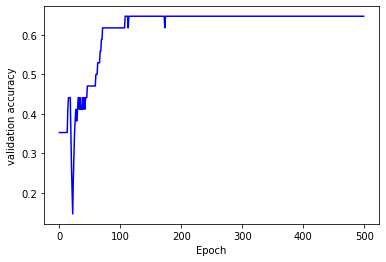
\includegraphics[width = 0.65 \textwidth]{Images/val_accuracy.png}
    \caption{Graph showing the trend of validation accuracy}
    \label{fig:val_accuracy}
\end{figure}

%\begin{figure}
%     \centering
%     \begin{subfigure}[b]{0.45\textwidth}
%         \centering
%         \includegraphics[width=\textwidth]{z_1.png}
%     \end{subfigure}
%     \hfill
%     \begin{subfigure}[b]{0.45\textwidth}
%         \centering
%         \includegraphics[width=\textwidth]{z_3.png}
%     \end{subfigure}
%\end{figure}
%\begin{figure}
%     \centering
%     \begin{subfigure}[b]{0.45\textwidth}
%         \centering
%         \includegraphics[width=\textwidth]{z_60.png}
%     \end{subfigure}
%     \hfill
%     \begin{subfigure}[b]{0.45\textwidth}
%         \centering
%         \includegraphics[width=\textwidth]{z_110.png}
%     \end{subfigure}
%     \caption{Four figures representing node embeddings at four different epochs}
%     \label{fig:4_embedding}
%\end{figure}

\begin{figure}
    \centering
    \begin{subfigure}{.45 \textwidth}
        \centering
        \includegraphics[width=\textwidth]{Images/z_1.png}
    \end{subfigure}
    \hfill
    \begin{subfigure}[b!]{0.45\textwidth}
        \centering
        \includegraphics[width=\textwidth]{Images/z_3.png}
    \end{subfigure}
    \begin{subfigure}[b]{0.45\textwidth}
        \centering
        \includegraphics[width=\textwidth]{Images/z_60.png}
    \end{subfigure}
    \hfill
    \begin{subfigure}[b]{0.45\textwidth}
        \centering
        \includegraphics[width=\textwidth]{Images/z_110.png}
    \end{subfigure}
    \caption{Four figures representing node embeddings at four different epochs}
    \label{fig:4_embedding}
\end{figure}


\chapter*{Conclusion}
\addcontentsline{toc}{chapter}{Conclusion}
\label{cap:conclusion}

Thanks to the easy availability of computing resources and datasets, as well as the rapid development in deep learning technologies on domain such as texts, images and videos, geometric deep learning methods have achieved great success in theoretical research and applications.
In this thesis, we have seen the process of diffusion on graphs and some graph neural networks such as graph attention networks.
We have also implemented a graphSAGE convolutional network for the task of node classification on the Zachary Karate Club dataset able to correctly classify $64.71\%$ of the nodes.
However, W. Hamilton \textit{et al.} in the paper \cite{graphsage} manage to reach an accuracy of $90.8\%$ with a graphSAGE convolution network on the Reddit dataset.
Furthermore, since geometric data is ubiquitous in the real life, geometric deep learning has the potential to find exciting new applications fields and to become the leading technology in machine learning in the near future.

\appendix

\chapter{Code}
\label{app:code}

First of all, we have to import all the packages that we are going to need.
\begin{lstlisting}
import torch
print("PyTorch has version {}".format(torch.__version__))

# Install torch geometric
!pip install -q torch-scatter -f https://pytorch-geometric.com/whl/torch-1.11.0+cu113.html
!pip install -q torch-sparse -f https://pytorch-geometric.com/whl/torch-1.11.0+cu113.html
!pip install -q torch-geometric

>>>PyTorch has version 1.11.0+cu113
\end{lstlisting}

\section{Upload dataset}
\label{sec:upload_dataset}

We then define a function useful for the sake of visualization.
\begin{lstlisting}
# Helper function for visualization.
%matplotlib inline
import torch
import networkx as nx
import matplotlib.pyplot as plt

# Visualization function for NX graph or PyTorch tensor
def visualize(h, color, epoch=None, loss=None, accuracy=None):
    plt.figure(figsize=(7,7))
    plt.xticks([])
    plt.yticks([])

    if torch.is_tensor(h):
        h = h.detach().cpu().numpy()
        plt.scatter(h[:, 0], h[:, 1], s=140, c=color, cmap="Set2")
        if epoch is not None and loss is not None and accuracy['train'] is not None and accuracy['val'] is not None:
            plt.xlabel((f'Epoch: {epoch}, Loss: {loss.item():.4f} \n'
                       f'Training Accuracy: {accuracy["train"]*100:.2f}% \n'
                       f' Validation Accuracy: {accuracy["val"]*100:.2f}%'),
                       fontsize=16)
    else:
        nx.draw_networkx(G, pos=nx.spring_layout(G, seed=42), with_labels=False,
                         node_color=color, cmap="Set2")
    plt.show()
\end{lstlisting}

We now access the dataset via the \lstinline{torch_geometric.datasets} subpackage:
\begin{lstlisting}
from torch_geometric.datasets import KarateClub

dataset = KarateClub()
print(f'Dataset: {dataset}:')
print('======================')
print(f'Number of graphs: {len(dataset)}')
print(f'Number of features: {dataset.num_features}')
print(f'Number of classes: {dataset.num_classes}')

>>>Dataset: KarateClub():
   ======================
   Number of graphs: 1
   Number of features: 34
   Number of classes: 4
\end{lstlisting}

After initializing the \lstinline{KarateClub()} dataset, we inspect some of its properties:
\begin{lstlisting}
data = dataset[0]  # Get the first graph object.

print(data)
print('==============================================================')

# Gather some statistics about the graph.
print(f'Number of nodes: {data.num_nodes}')
print(f'Number of edges: {data.num_edges}')
print(f'Average node degree: {data.num_edges / data.num_nodes:.2f}')
print(f'Number of training nodes: {data.train_mask.sum()}')
print(f'Training node label rate: {int(data.train_mask.sum()) / data.num_nodes:.2f}')
print(f'Contains isolated nodes: {data.contains_isolated_nodes()}')
print(f'Contains self-loops: {data.contains_self_loops()}')
print(f'Is undirected: {data.is_undirected()}')

>>>Data(x=[34, 34], edge_index=[2, 156], y=[34], train_mask=[34])
   ==============================================================
   Number of nodes: 34
   Number of edges: 156
   Average node degree: 4.59
   Number of training nodes: 4
   Training node label rate: 0.12
   Contains isolated nodes: False
   Contains self-loops: False
   Is undirected: True
\end{lstlisting}

We can visualize the graph by converting it to the \lstinline{networkx} library format:
\begin{lstlisting}
from torch_geometric.utils import to_networkx

G = to_networkx(data, to_undirected=True)
visualize(G, color=data.y)
\end{lstlisting}
\begin{figure}[h]
    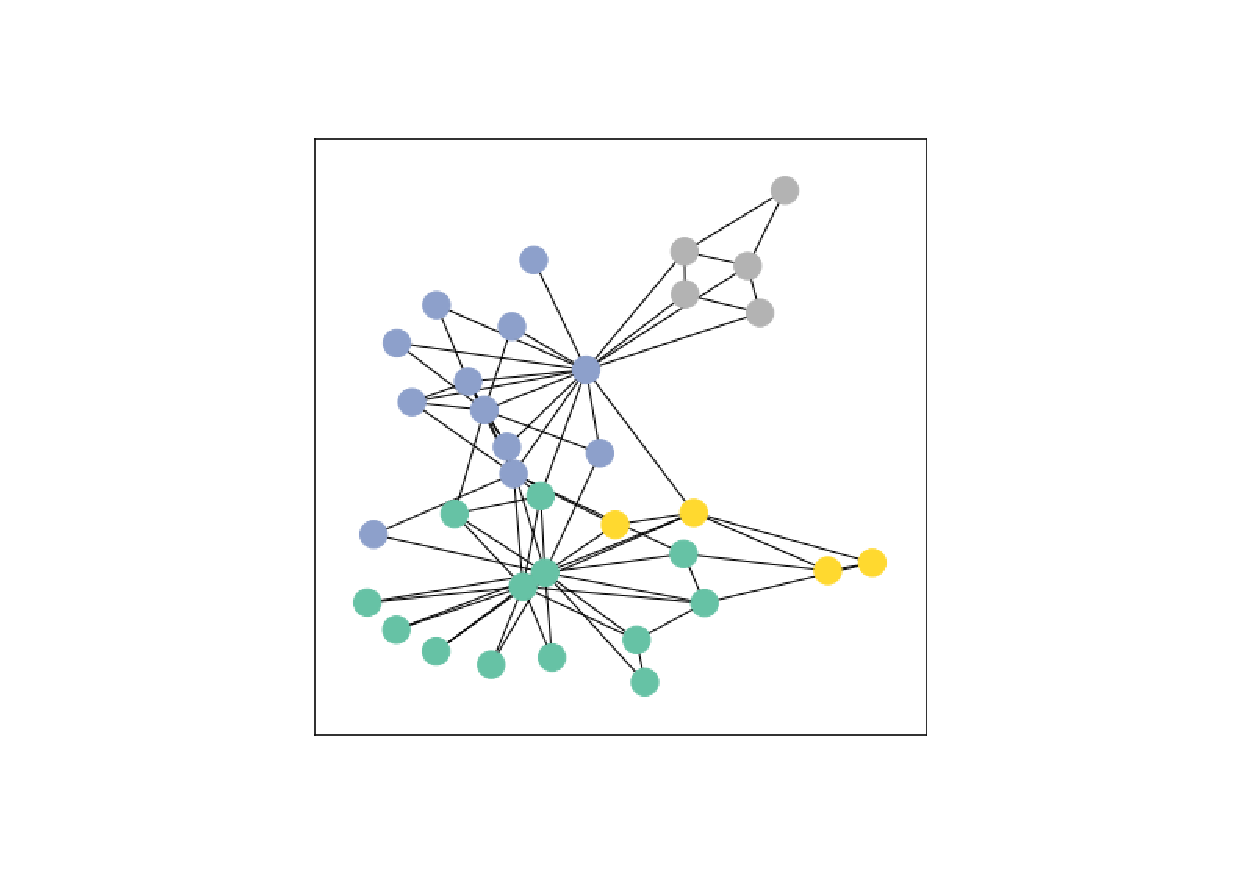
\includegraphics[width = 0.5 \textwidth, trim={4.5cm 2.2cm 4.5cm 2.2cm}, clip]{Images/zachary_py.pdf}
    %\caption{Caption}
    %\label{fig:my_label}
\end{figure}

\section{Code's architecture}
\label{sec:code_arch}

\begin{lstlisting}
import torch_geometric
torch_geometric.__version__

import torch_scatter
import torch.nn as nn
import torch.nn.functional as F

import torch_geometric.nn as pyg_nn
import torch_geometric.utils as pyg_utils

from torch import Tensor
from typing import Union, Tuple, Optional
from torch_geometric.typing import (OptPairTensor, Adj, Size, NoneType,
                                    OptTensor)

from torch.nn import Parameter, Linear
from torch_sparse import SparseTensor, set_diag
from torch_geometric.nn.conv import MessagePassing
from torch_geometric.utils import remove_self_loops, add_self_loops, softmax

import time

import networkx as nx
import numpy as np
import torch
import torch.optim as optim

from torch_geometric.datasets import TUDataset
from torch_geometric.datasets import Planetoid
from torch_geometric.data import DataLoader

import torch_geometric.nn as pyg_nn

import matplotlib.pyplot as plt

from torch.nn import Linear
from torch_geometric.nn import SAGEConv


class GraphSageConv(torch.nn.Module):
    def __init__(self, input_dim, hidden_dim, output_dim,
                 ):
        super(GraphSageConv, self).__init__()
        self.conv1 = SAGEConv(input_dim, hidden_dim, normalize=True)
        self.conv2 = SAGEConv(hidden_dim, hidden_dim, normalize=True)
        self.conv3 = SAGEConv(hidden_dim, 2, normalize=True)
        self.classifier = Linear(2, output_dim)

    # Define the forward pass
    def forward(self, x, edge_index):
        h = self.conv1(x, edge_index)
        h = h.tanh()
        h = self.conv2(h, edge_index)
        h = h.tanh()
        h = self.conv3(h, edge_index)
        h = h.tanh() # Final GNN embedding space: h is the matrix of the node embeddings computed by our encoder which is the composition of 3 GraphSage layers!

        if self.training:
                x1 = h 
                h = x1
        
        # Apply a final linear classifier.
        out = self.classifier(h)

        return out, h

\end{lstlisting}

\section{Training}
\label{sec:training}

\begin{lstlisting}
model = GraphSageConv(dataset.num_features, 4, dataset.num_classes)
criterion = torch.nn.CrossEntropyLoss()  # Define loss criterion.
optimizer = torch.optim.Adam(model.parameters(), lr=0.01)  # Define optimizer.

def train(data):
    optimizer.zero_grad()  # Clear gradients.
    out, h = model(data.x, data.edge_index)  # Perform a single forward pass.
    loss = criterion(out[data.train_mask], data.y[data.train_mask])  # Compute the loss solely based on the training nodes.
    loss.backward()  # Derive gradients.
    optimizer.step()  # Update parameters based on gradients.


    accuracy = {}
    # Calculate training accuracy on our four examples
    predicted_classes = torch.argmax(out[data.train_mask], axis=1)
    target_classes = data.y[data.train_mask]
    accuracy['train'] = torch.mean(
        torch.where(predicted_classes == target_classes, 1, 0).float())
    
    # Calculate validation accuracy on the whole graph
    predicted_classes = torch.argmax(out, axis=1)
    target_classes = data.y
    accuracy['val'] = torch.mean(
        torch.where(predicted_classes == target_classes, 1, 0).float())

    return loss, h, accuracy

accuracies = []
epochs = []
for epoch in range(500):
    loss, h, accuracy = train(data)
    accuracies.append(accuracy["val"])
    epochs.append(epoch)
    # Visualize the node embeddings every 10 epochs
    if epoch % 10 == 0:
        visualize(h, color=data.y, epoch=epoch, loss=loss, accuracy=accuracy)
        time.sleep(0.3)
        
plot=plt.figure(1)
plt.plot(epochs, accuracies, color="blue")
plt.ylabel('validation accuracy')
plt.xlabel('Epoch')
plt.show()
\end{lstlisting}


\printbibliography[heading=bibintoc]

\chapter*{Ringraziamenti}
\addcontentsline{toc}{chapter}{Ringraziamenti}

Questa tesi rappresenta la conclusione di un percorso formativo durato tre anni, che mi ha permesso di costruire nuovi rapporti, sia dentro e fuori l'ambiente accademico.

Innanzitutto, vorrei ringraziare la Prof.ssa Rita Fioresi, che è stata di grande aiuto in quest'ultimo anno.
Infatti, oltre ad avermi introdotto nel mondo del geometric deep learning ed ad aver permesso la realizzazione di questa tesi, in molte occasioni i suoi consigli si sono rivelati fondamentali nell'orientamento dei miei futuri studi.
Inoltre, è stata di sostanziale importanza nella scelta e nell'ammissione del master, e per questo le sono grato.
Ringrazio inoltre Ferdinando Zanchetta per le lezioni introduttorie al geometric deep learning che mi hanno aiutato a velocizzare molto il mio studio e l'attuazione di questa tesi.

Successivamente vorrei ringraziare la mia famiglia, che mi ha sempre sostenuto durante gli studi e mi ha sempre spinto a sfruttare tutte le possibilità che mi venivano offerte.

È d'obbligo a questo punto nominare il gruppo studio Qualcosa, senza il quale non avrei avuto la possibilità di confrontarmi su argomenti di elevata importanza accademica e notevole complessità.
In particolare ringrazio di cuore, in ordine, i membri del gruppo:
Sere, che in molte, molte occasioni è riuscita ad evitare dei litigi interni al gruppo e a rasSEREnare la situazione, e infine
Dani, 
%\href{https://it.wikipedia.org/wiki/Coglione}{Dani}, 
il quale non è che abbia portato molti contributi allo studio, ma comunque è stata un presenza importante (BNF).

Infine, vorrei ringraziare due persone distanti dal mondo accademico della fisica, ma che comunque si sono rivelate essenziali durante il mio percorso.
Il primo ringraziamento speciale va all'Ali, che mi ha sempre spinto a dare il meglio di me, sia all'università sia fuori.
%Prima di tutto l'Ali, che ha sopportato tutte le mie lamentele pre- e post-esame della triennale, e in generale è da quattro anni che mi tollera e non so se è più adeguato dire `grazie' o `scusa'.
Ultimo ringraziamento è ovviamente per Chucky.

\end{document}
